\documentclass[letterpaper,journal]{IEEEtran}

\usepackage{amsmath,amssymb}
\usepackage{booktabs}
\usepackage{cite}
\usepackage{graphicx}
\usepackage{multirow}
\usepackage{url}
\usepackage{stfloats}

\begin{document}

\title{Diffusion-Driven Graph Reconstruction and Cross-View Contrastive Learning for Bundle Recommendation}

% Four fictional authors and one assumed shared affiliation for layout testing.
\author{***, ***, ***, and ***%
\thanks{Layout preview with fictional authors and biographies. Corresponding author: ***.}%
\thanks{The authors are with Anhui University, Hefei, China (e-mail: author@example.org).}}

% Alternative first-page layout for visual comparison only.
\newcommand{\frontbio}[2]{%
  \begin{minipage}[t]{\columnwidth}
  \noindent\begin{minipage}[t]{1in}\vspace{0pt}%
  {\setlength{\fboxsep}{0pt}\fbox{\parbox[c][\dimexpr1.25in-2\fboxrule\relax][c]{\dimexpr1in-2\fboxrule\relax}{\centering\footnotesize PLACE\\PHOTO\\HERE}}}%
  \end{minipage}\hfill
  \begin{minipage}[t]{\dimexpr\linewidth-1in-0.12in\relax}\vspace{0pt}%
  \footnotesize\textbf{#1} #2\par
  \end{minipage}%
  \end{minipage}}
\IEEEaftertitletext{%
  \noindent\frontbio{***}{is a graduate student at Anhui University, Hefei, China. Her research focuses on graph-based recommendation and the evaluation of ranking models under sparse user feedback. She is interested in how item-level interactions can help a model learn which bundles a user prefers.}\hfill
  \frontbio{***}{received the M.S. degree in software engineering from Northmere University in 2021. He is currently pursuing the Ph.D. degree at Anhui University, Hefei, China. His research interests include representation learning on graphs, implicit feedback, and the reproducibility of recommendation experiments.}\par\vspace{10pt}
  \noindent\frontbio{***}{received the Ph.D. degree in computer science from Lakebridge University in 2016. He is an Associate Professor at Anhui University, Hefei, China. His research interests include information retrieval and machine learning. He studies how changes in user behavior affect the quality of ranked results over time.}\hfill
  \frontbio{***}{received the Ph.D. degree in information science from Northmere University in 2013. She is a Professor at Anhui University, Hefei, China. Her research interests include personalized recommendation, user modeling, and graph learning. Her recent work examines how item interactions can help model preferences for collections of items.}\par\vspace{10pt}}

\maketitle

\begin{abstract}
Bundle recommendation (BR) aims to match users with collections of items that suit their preferences. Existing graph-based methods learn bundle preferences primarily from user-bundle (U-B) interactions, while incorporating user-item (U-I) interactions and bundle-item (B-I) affiliations as auxiliary information. Despite their effectiveness, limitations in the observed U-B interactions still pose two challenges: (1) noise in the observed U-B graph can introduce misleading preference signals during graph propagation; (2) sparse U-B feedback hinders accurate modeling of users' bundle preferences. To address these challenges, we propose Reconstruction and Contrastive Learning for Bundle Recommendation (ReCoBR). Specifically, ReCoBR reduces the impact of noisy interactions through Pretraining-Based Diffusion-Driven U-B Graph Reconstruction (PDGR) and improves preference learning under sparse feedback through Cross-View Contrastive Learning (CCL). In PDGR, we combine graph pretraining with user-conditioned diffusion to generate reliability scores for observed U-B interactions, incorporating a bundle-set consistency loss to preserve historical preference signals. We then retain high-scoring interactions to effectively denoise and reconstruct the U-B graph. Next, CCL applies contrastive learning between the reconstructed U-B view and each auxiliary view before representation fusion, introducing explicit cross-view constraints that enable auxiliary information to better support bundle preference learning for sparse users. Experiments on three public datasets show that ReCoBR outperforms the baseline methods.
\end{abstract}

\begin{IEEEkeywords}
Bundle recommendation, contrastive learning, diffusion models, graph reconstruction.
\end{IEEEkeywords}

\section{Introduction}

\IEEEPARstart{B}{undle} recommendation (BR) aims to match users with collections of related items, such as music playlists and fashion outfits~\cite{chen2019dam,ma2022crosscbr}. BR helps users discover suitable collections while creating additional sales opportunities for platforms~\cite{ma2022crosscbr,ma2024multicbr}. To learn users' bundle preferences, BR methods commonly use three types of relations~\cite{ma2022crosscbr,ma2024multicbr}: user-bundle (U-B) interactions reflect users' choices of bundles; user-item (U-I) interactions provide information about their interests in individual items; and bundle-item (B-I) affiliations describe which items belong to each bundle. Together, these relations provide information for learning users' bundle preferences.

Early BR methods explored how to incorporate item-level information into bundle preference learning~\cite{liu2014lire,pathak2017bundlebpr}. For example, DAM jointly models U-B and U-I interactions, using attention to construct bundle representations from item embeddings~\cite{chen2019dam}. To capture higher-order relations among users, bundles, and items, BGCN introduces graph propagation in the bundle and item views~\cite{chang2020bgcn}. BGCN also uses B-I affiliations to aggregate item information into bundle representations. Building on multi-view representation learning, subsequent studies have focused on strengthening information exchange and integration across views. For instance, CrossCBR applies contrastive learning to align representations of the same user (bundle) across the bundle and item views~\cite{ma2022crosscbr}. Meanwhile, DGMAE uses knowledge distillation to transfer information from first- and higher-order U-B relations to the item view~\cite{ren2023dgmae}. More recently, MultiCBR separately learns representations from the U-B, U-I, and B-I views, fuses these representations for recommendation, and applies contrastive learning after fusion~\cite{ma2024multicbr}. Recent studies have also investigated diffusion models to improve user and bundle representations for recommendation. Specifically, DCDL applies diffusion learning to user representations within a dual-view framework to improve recommendation diversity~\cite{chen2025dcdl}. In addition, RDiffBR uses residual diffusion to adapt bundle representations to changes in bundle composition~\cite{zhang2026rdiffbr}.

Although these methods differ in their modeling strategies, they focus on extracting preference signals from interaction data~\cite{ma2024multicbr} and largely overlook the limitations of U-B feedback. In particular, noise and sparsity in the observed U-B interactions remain significant obstacles to accurately modeling users' bundle preferences. For example, accidental clicks may be recorded as positive interactions even when they do not reflect users' actual preferences~\cite{jiang2026cafu}. During graph propagation, misleading preference signals from noisy U-B interactions can spread through neighborhood aggregation~\cite{wu2021sgl}. Meanwhile, many users have interacted with only a few bundles, leaving limited historical information for learning their preferences~\cite{chang2020bgcn}. For these sparse users, U-I interactions and B-I affiliations can provide additional information, but effectively using this information for bundle preference learning remains difficult. Based on the above analysis, we identify the following two challenges.

\textbf{Challenge 1: Denoising U-B Feedback While Preserving Preference Information.} The observed U-B graph does not indicate which connections are noisy, making it difficult to decide which ones to retain for graph propagation. Retaining unreliable connections may allow misleading preference signals to spread through neighborhood aggregation. However, removing too many connections can also discard valuable information about users' historical bundle choices. Therefore, we need to develop an effective mechanism for assessing the reliability of observed U-B interactions to guide graph denoising.

\textbf{Challenge 2: Cross-View Collaboration under Sparse U-B Feedback.} Sparse U-B interactions hinder accurate modeling of users' bundle preferences~\cite{yu2022uhbr,jiang2026mgcbr}. To alleviate U-B sparsity, it is important to effectively use the additional information provided by U-I interactions and B-I affiliations. Existing three-view methods such as MultiCBR separately learn representations through graph propagation in each view and integrate these representations through weighted fusion~\cite{ma2024multicbr}. However, simple weighted fusion lacks explicit cross-view constraints that can provide additional supervision for preference learning under sparse U-B feedback. This limitation highlights the need to make more effective use of information from the U-I and B-I views to improve bundle preference learning for sparse users.

To address these challenges, we propose \textbf{Reconstruction and Contrastive Learning for Bundle Recommendation (ReCoBR)}, which comprises Pretraining-Based Diffusion-Driven U-B Graph Reconstruction (PDGR) and Cross-View Contrastive Learning (CCL). PDGR provides a diffusion-driven mechanism to assess the reliability of observed U-B interactions and guide graph denoising. Specifically, we use LightGCN~\cite{he2020lightgcn} pretraining to derive user preference representations from bundle interaction histories. Next, we use a diffusion model conditioned on the pretrained user embeddings to denoise these preference representations. During denoising, we introduce a bundle-set consistency loss (SetLoss) to preserve useful preference information by aligning the denoised preferences with users' historical bundle embeddings. Finally, we score the observed U-B interactions using the denoised preferences and retain high-scoring connections to reconstruct the graph for propagation. Building on the reconstructed U-B graph, CCL offers additional supervision for preference learning under sparse U-B feedback. Specifically, we apply contrastive learning before fusion to align representations of the same user (bundle) between the reconstructed U-B view and each auxiliary view. These constraints use auxiliary information to directly guide U-B representation learning, compensating for the limited supervision from sparse users' bundle interactions. Overall, ReCoBR establishes a unified framework that integrates diffusion and cross-view contrastive learning to effectively address noise and sparsity in U-B interactions.

Our main contributions are summarized as follows:

\begin{enumerate}
\item We propose a bundle recommendation framework, ReCoBR, which uses diffusion-driven U-B graph reconstruction based on pretrained embeddings to reduce the impact of noisy interactions.
\item We design cross-view contrastive learning based on the reconstructed U-B view, enabling more effective use of auxiliary information to improve bundle preference learning for sparse users.
\item We conduct extensive experiments on three public datasets and show that ReCoBR improves bundle recommendation performance by mitigating the effects of noise and sparsity in U-B interactions.
\end{enumerate}

\begin{figure*}[!t]
    \centering
    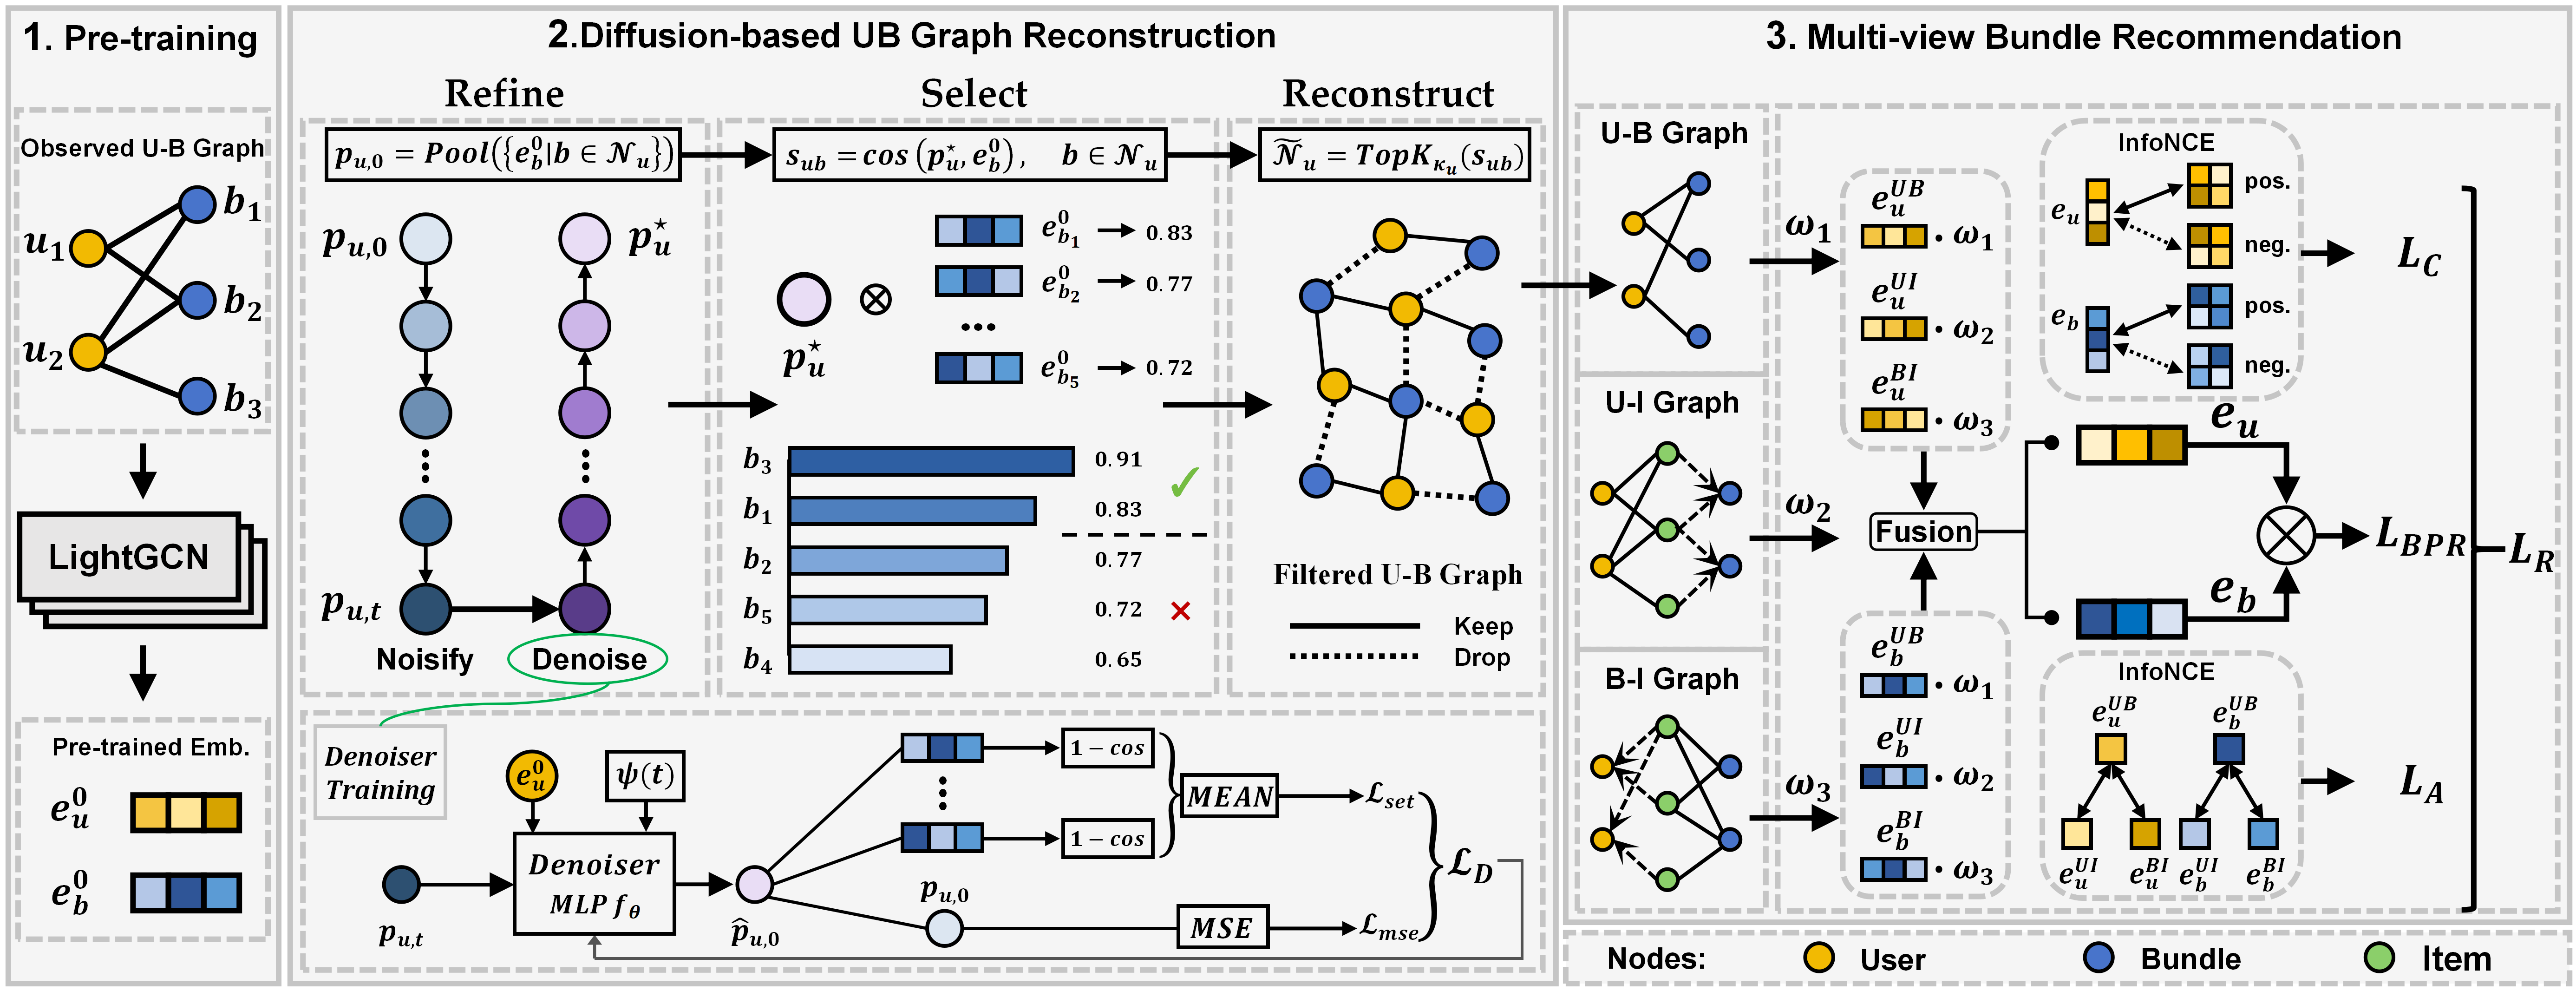
\includegraphics[width=0.98\textwidth]{Figures/digo_framework.png}
    \caption{Overall framework of ReCoBR. PDGR reconstructs the U-B graph using pretrained embeddings and user-conditioned diffusion. The denoiser is trained with reconstruction and bundle-set consistency losses. CCL applies cross-view contrastive learning before representation fusion. Pool denotes mean pooling.}
    \label{fig:framework}
\end{figure*}

\section{Related Work}

\subsection{Bundle Recommendation}

Bundle recommendation includes both ranking predefined bundles and constructing new item collections~\cite{sun2024survey}. For bundle ranking, early methods connect users' bundle choices with their item interests through factorization models~\cite{cao2017efm} or attention-based aggregation in DAM~\cite{chen2019dam}. Graph-based methods further capture higher-order relations among users, bundles, and items. For example, BGCN propagates information at both the bundle and item levels to learn user and bundle representations~\cite{chang2020bgcn}.

Later studies seek richer preference representations by modeling user intents and bundle structure or by exploiting additional collaborative information. MIDGN disentangles user intents across and within bundles~\cite{zhao2022midgn}, while BundleGT models item associations within bundles using a hierarchical graph Transformer~\cite{wei2023bundlegt}. To strengthen item-level representations, DGMAE transfers knowledge of first- and higher-order U-B relations to the item view through knowledge distillation~\cite{ren2023dgmae}. EBRec also uses bundle--user--item correlations and augmented U-I interactions to enrich item-level bundle representations~\cite{du2025ebrec}. EpicCBR mines item relations from U-I interactions and B-I affiliations to enhance the U-I view, then uses multi-view contrastive learning to improve user and bundle representations~\cite{li2026epiccbr}.

\subsection{Denoising and Diffusion for Recommendation}

Denoising methods seek to reduce the influence of noisy implicit feedback on preference learning. ADT filters or downweights high-loss interactions~\cite{wang2021adt}, while DeCA uses agreement between model predictions to guide denoising~\cite{wang2022deca}. At the representation level, CAFU reduces noise through filtered uniformity and improves learning for sparse users through constrained alignment~\cite{jiang2026cafu}.

Diffusion models offer a different approach by learning to reconstruct data or representations corrupted by added noise~\cite{ho2020ddpm}. DiffRec applies this process to user interaction vectors~\cite{wang2023diffrec}, whereas DiffuRec reconstructs target-item embeddings for sequential recommendation~\cite{li2023diffurec}. To improve robustness against noisy feedback, DDRM applies diffusion denoising to user and item embeddings~\cite{zhao2024ddrm}.

In bundle recommendation, diffusion has been explored to improve diversity and robustness. DCDL denoises user representations with guidance from fused user features to improve recommendation diversity~\cite{chen2025dcdl}. RDiffBR instead focuses on changes in bundle composition, using residual diffusion to adapt item-level bundle representations~\cite{zhang2026rdiffbr}. ReCoBR applies diffusion to historical preference representations and uses the denoised preferences to filter observed U-B interactions for graph propagation.

\subsection{Contrastive Learning for Recommendation}

Contrastive learning provides additional supervision by bringing positive pairs closer and pushing negative pairs apart in the representation space~\cite{chen2020simclr}. In graph-based recommendation, SGL constructs contrastive views through random graph augmentations, including node and edge dropout~\cite{wu2021sgl}. To make view construction adaptive, AdaGCL uses trainable graph generation and denoising models~\cite{jiang2023adagcl}. For intent modeling, BIGCF applies contrastive regularization to both interaction and intent representations~\cite{zhang2024bigcf}.

In bundle recommendation, CrossCBR aligns representations of the same user (bundle) across the bundle and item views before fusion~\cite{ma2022crosscbr}. In contrast, MultiCBR applies contrastive learning to the fused representations of the U-B, U-I, and B-I views~\cite{ma2024multicbr}. ReCoBR adds contrastive learning between the reconstructed U-B view and each auxiliary view before fusion, while retaining the post-fusion contrastive objective.

\section{Methodology}\label{sec:methodology}

ReCoBR combines U-B graph reconstruction with cross-view contrastive learning (Fig.~\ref{fig:framework}). PDGR first scores observed U-B interactions and retains high-scoring connections to reconstruct the U-B graph. CCL then applies contrastive learning between the reconstructed U-B view and each auxiliary view (U-I and B-I) before representation fusion.

\subsection{Task Definition}

Let $\mathcal U$, $\mathcal B$, and $\mathcal I$ denote the sets of users, predefined bundles, and items, respectively. The available training data comprise three binary matrices: user-bundle interactions $\mathbf X\in\{0,1\}^{|\mathcal U|\times|\mathcal B|}$, user-item interactions $\mathbf Y\in\{0,1\}^{|\mathcal U|\times|\mathcal I|}$, and bundle-item affiliations $\mathbf Z\in\{0,1\}^{|\mathcal B|\times|\mathcal I|}$. In $\mathbf X$ and $\mathbf Y$, an entry equal to one denotes an observed interaction; in $\mathbf Z$, it denotes bundle membership. Given these relations, our task is to estimate a preference score $\hat y_{ub}$ for each unobserved user-bundle pair and rank candidate bundles for each user. We distinguish the observed matrix $\mathbf X$ from the reconstructed matrix $\widetilde{\mathbf X}$ throughout this section. The former defines users' training histories and ranking examples; the latter determines the U-B connections used for recommendation graph propagation.

\subsection{Pretraining-Based Diffusion-Driven U-B Graph Reconstruction (PDGR)}\label{sec:graph-reconstruction}

PDGR assesses the reliability of observed U-B interactions through preference-based scoring. We construct historical preference representations from pretrained embeddings and train a user-conditioned denoiser with a bundle-set consistency constraint. The refined preferences are then used to score observed interactions and retain high-scoring connections for graph propagation.

\subsubsection{Pretraining and Historical Preference Construction}

To capture collaborative information from U-B interactions, we pretrain LightGCN \cite{he2020lightgcn} on the observed U-B graph using Bayesian Personalized Ranking (BPR) \cite{rendle2009bpr}. Let $\mathbf h_u^{(0)},\mathbf h_b^{(0)}\in\mathbb R^d$ denote the trainable initial embeddings. The observed neighbors of user $u$ and bundle $b$ are $\mathcal N_u=\{b\in\mathcal B:x_{ub}=1\}$ and $\mathcal N_b=\{u\in\mathcal U:x_{ub}=1\}$, respectively. LightGCN propagates information between users and bundles as follows:
\begin{equation}
\begin{aligned}
\mathbf h_u^{(k+1)}
&=\sum_{b\in\mathcal N_u}
\frac{\mathbf h_b^{(k)}}
{\sqrt{|\mathcal N_u||\mathcal N_b|}},\\
\mathbf h_b^{(k+1)}
&=\sum_{u\in\mathcal N_b}
\frac{\mathbf h_u^{(k)}}
{\sqrt{|\mathcal N_b||\mathcal N_u|}}.
\end{aligned}
\tag{1}
\end{equation}
After $K_p$ propagation layers, we average the initial and propagated embeddings to obtain the pretrained user and bundle embeddings:
\begin{equation}
\mathbf e_u^0=\frac{1}{K_p+1}\sum_{k=0}^{K_p}\mathbf h_u^{(k)},
\qquad
\mathbf e_b^0=\frac{1}{K_p+1}\sum_{k=0}^{K_p}\mathbf h_b^{(k)}.
\tag{2}
\end{equation}
The pretrained embeddings remain fixed throughout denoiser and recommendation training. We use $\mathbf e_b^0$ to construct historical preference representations and score observed interactions, while $\mathbf e_u^0$ provides the user condition for denoising.

We construct historical preference representations for users with observed U-B interactions, denoted by $\mathcal U_+=\{u\in\mathcal U:|\mathcal N_u|>0\}$. For each $u\in\mathcal U_+$, we average the pretrained embeddings of their historically interacted bundles:
\begin{equation}
\mathbf p_{u,0}
=\frac{1}{|\mathcal N_u|}
\sum_{b\in\mathcal N_u}\mathbf e_b^0.
\tag{3}
\end{equation}
The resulting vector $\mathbf p_{u,0}$ summarizes the user's historical bundle preferences. Mean pooling maps histories of different lengths to a $d$-dimensional representation. The subscript $0$ denotes the preference representation before Gaussian noise is added.

\subsubsection{User-Conditioned Diffusion Denoising}

We train the denoiser to recover historical preference representations from inputs with different noise levels. Following the Gaussian diffusion formulation \cite{ho2020ddpm,wang2023diffrec}, let $T$ be the number of diffusion steps and $\beta_t\in(0,1)$ the noise variance at step $t$. We use a linear variance schedule, with $\alpha_t=1-\beta_t$ and $\bar\alpha_t=\prod_{s=1}^{t}\alpha_s$. At step $t$, the noisy preference representation is
\begin{equation}
\mathbf p_{u,t}
=\sqrt{\bar\alpha_t}\,\mathbf p_{u,0}
+\sqrt{1-\bar\alpha_t}\,\boldsymbol\epsilon,
\qquad
\boldsymbol\epsilon\sim\mathcal N(\mathbf 0,\mathbf I_d).
\tag{4}
\end{equation}
Here, $\boldsymbol\epsilon\in\mathbb R^d$ is standard Gaussian noise, and $\mathbf I_d$ is the $d$-dimensional identity matrix. The coefficient $\bar\alpha_t$ controls the contribution of the historical preference representation at step $t$.

Following DiffRec~\cite{wang2023diffrec} and DimeRec~\cite{li2025dimerec}, we use a multilayer perceptron (MLP) as the denoiser. At step $t$, the denoiser uses the pretrained user embedding $\mathbf e_u^0$ to recover the user's historical preference representation from the noisy input $\mathbf p_{u,t}$. To compare the two vectors, we compute their element-wise product and absolute difference and concatenate the results into a feature vector $\mathbf m_{u,t}$:
\begin{equation}
\mathbf m_{u,t}
=\bigl[\mathbf p_{u,t}\odot\mathbf e_u^0\,;\,
\lvert\mathbf p_{u,t}-\mathbf e_u^0\rvert\bigr].
\tag{5}
\end{equation}
Here, $\odot$ denotes element-wise multiplication and $[\,\cdot\,;\,\cdot\,]$ denotes concatenation. The MLP combines the two original vectors with $\mathbf m_{u,t}$ and a sinusoidal timestep embedding that indicates the noise level. We denote the resulting denoiser by $f_\theta$ and its estimate of the historical preference representation by $\widehat{\mathbf p}_{u,0}$:
\begin{equation}
\widehat{\mathbf p}_{u,0}
=f_\theta(\mathbf p_{u,t},\mathbf e_u^0,t).
\tag{6}
\end{equation}

During training, we uniformly sample a user $u\in\mathcal U_+$ and a timestep $t\in\{1,\ldots,T\}$. We then sample Gaussian noise to construct $\mathbf p_{u,t}$ as in Eq. (4). We use the mean squared error (MSE)~\cite{wang2009mse} as the reconstruction loss:
\begin{equation}
\mathcal L_{\mathrm{mse}}
=\mathbb E_{u,t,\boldsymbol\epsilon}
\left[
\frac{1}{d}
\left\|\widehat{\mathbf p}_{u,0}-\mathbf p_{u,0}\right\|_2^2
\right].
\tag{7}
\end{equation}
Minimizing this loss trains the denoiser to recover $\mathbf p_{u,0}$ from $\mathbf p_{u,t}$, with $\mathbf e_u^0$ providing user-specific information.

\subsubsection{Bundle-Set Consistency in Denoising}

The reconstruction loss in Eq. (7) supervises recovery of the pooled historical preference vector. Graph reconstruction, however, requires scoring each historical bundle against the denoised preference. We therefore introduce a bundle-set consistency loss (SetLoss) to preserve useful preference information from the user's historical bundles. SetLoss encourages consistency between the denoised preference and the user's historical bundle embeddings:
\begin{equation}
\mathcal L_{\mathrm{set}}
=\mathbb E_{u,t,\boldsymbol\epsilon}
\left[
\frac{1}{|\mathcal N_u|}
\sum_{b\in\mathcal N_u}
\left(1-\cos
\left(\widehat{\mathbf p}_{u,0},\mathbf e_b^0\right)\right)
\right].
\tag{8}
\end{equation}
Here, $\cos(\mathbf a,\mathbf b)=\mathbf a^\top\mathbf b/(\|\mathbf a\|_2\|\mathbf b\|_2)$ denotes cosine similarity. SetLoss and interaction scoring use the same cosine similarity, linking preference denoising to graph reconstruction. We jointly optimize the two losses:
\begin{equation}
\mathcal L_{\mathrm D}
=\mathcal L_{\mathrm{mse}}
+\lambda_{\mathrm{set}}\mathcal L_{\mathrm{set}},
\tag{9}
\end{equation}
where $\lambda_{\mathrm{set}}\geq 0$ controls the contribution of SetLoss.

\subsubsection{Preference Refinement and Graph Reconstruction}

To reconstruct the U-B graph, we apply the current denoiser to each user's historical preference representation. Starting from $\mathbf p_{u,0}$, we repeatedly update the representation over timesteps $T,T-1,\ldots,1$:
\begin{equation}
\begin{aligned}
\mathbf r_{u,T}&=\mathbf p_{u,0},\\
\mathbf r_{u,t-1}
&=f_\theta(\mathbf r_{u,t},\mathbf e_u^0,t),
\qquad t=T,T-1,\ldots,1,\\
\mathbf p_u^\star&=\mathbf r_{u,0}.
\end{aligned}
\tag{10}
\end{equation}
Here, $\mathbf r_{u,t}$ is the intermediate representation during refinement, and $\mathbf p_u^\star$ is the final refined preference. Each step passes the current representation, the pretrained user embedding, and the timestep to the denoiser.

We then score each observed U-B interaction by the cosine similarity between the refined preference and the corresponding pretrained bundle embedding:
\begin{equation}
s_{ub}
=\cos(\mathbf p_u^\star,\mathbf e_b^0),
\qquad b\in\mathcal N_u.
\tag{11}
\end{equation}
A higher score means that the bundle better matches the user's refined preference. For each user, we retain the highest-scoring $\kappa_u=\min(\kappa,|\mathcal N_u|)$ bundles. The positive integer $\kappa$ specifies the maximum number of retained interactions per user:
\begin{equation}
\begin{aligned}
\widetilde{\mathcal N}_u
&=\underset{b\in\mathcal N_u}{\operatorname{TopK}}
\left(s_{ub},\kappa_u\right),\\
\widetilde x_{ub}
&=\mathbf 1\!\left[b\in\widetilde{\mathcal N}_u\right].
\end{aligned}
\tag{12}
\end{equation}
Here, $\operatorname{TopK}(s_{ub},\kappa_u)$ returns the set of $\kappa_u$ bundles in $\mathcal N_u$ with the largest scores, and $\mathbf 1[\cdot]$ is the indicator function. Users with at most $\kappa$ observed bundles retain all their connections. The selected interactions form $\widetilde{\mathbf X}$, which defines the reconstructed U-B graph for propagation.

\subsection{Cross-View Contrastive Learning (CCL)}

Building on the reconstructed U-B graph, CCL uses the U-I and B-I views to provide additional supervision for bundle preference learning. We encode the three relation views, then align representations of the same user (bundle) between the reconstructed U-B view and each auxiliary view before fusion. These explicit cross-view constraints help auxiliary information support preference learning for sparse users.

\subsubsection{View-Specific Representations}

Following the three-view backbone of MultiCBR \cite{ma2024multicbr}, we construct the U-B, U-I, and B-I propagation graphs from $\widetilde{\mathbf X}$, $\mathbf Y$, and $\mathbf Z$, respectively. The encoders share trainable initial embeddings for the same entity. These embeddings are learned during recommendation training, separately from the fixed pretrained embeddings used by PDGR.

Each encoder applies $L$ layers of symmetrically normalized LightGCN-style propagation \cite{he2020lightgcn}. Within each view, fixed layer weights combine the initial embeddings and the $\ell_2$-normalized propagation outputs. During recommendation training, we perturb the output of each propagation layer before normalization. We apply the same rule after item pooling. For an output vector $\mathbf h$ computed using relation $g\in\{\mathrm{UB},\mathrm{UI},\mathrm{BI}\}$, the perturbed vector is
\begin{equation}
\widetilde{\mathbf h}
=\mathbf h+\rho_g\,\operatorname{sign}(\mathbf h)
\odot\frac{\boldsymbol\xi}{\|\boldsymbol\xi\|_2}.
\tag{13}
\end{equation}
Here, $\rho_g$ denotes the perturbation strength for relation $g$. The entries of $\boldsymbol\xi$ are sampled independently and uniformly from $[0,1)$, and $\operatorname{sign}(\cdot)$ acts element-wise. We omit the perturbation during evaluation.

\textbf{U-B view.} Propagation on the reconstructed U-B graph directly produces user representations $\mathbf e_u^{\mathrm{UB}}$ and bundle representations $\mathbf e_b^{\mathrm{UB}}$, capturing collaborative information through the retained interactions.

\textbf{U-I view.} Propagation on the U-I graph produces user representations $\mathbf e_u^{\mathrm{UI}}$ and item representations $\mathbf e_i^{\mathrm{UI}}$. To obtain a bundle representation $\mathbf e_b^{\mathrm{UI}}$ in this view, we average the representations of its constituent items according to $\mathbf Z$.

\textbf{B-I view.} Propagation on the B-I graph produces bundle representations $\mathbf e_b^{\mathrm{BI}}$ and item representations $\mathbf e_i^{\mathrm{BI}}$. To obtain a user representation $\mathbf e_u^{\mathrm{BI}}$ in this view, we average the representations of the items that the user has interacted with according to $\mathbf Y$.

The two item-pooling operations are
\begin{equation}
\mathbf e_b^{\mathrm{UI}}
=\frac{1}{|\mathcal I_b|}
\sum_{i\in\mathcal I_b}\mathbf e_i^{\mathrm{UI}},
\qquad
\mathbf e_u^{\mathrm{BI}}
=\frac{1}{|\mathcal I_u|}
\sum_{i\in\mathcal I_u}\mathbf e_i^{\mathrm{BI}},
\tag{14}
\end{equation}
where $\mathcal I_b=\{i:z_{bi}=1\}$ contains the items in bundle $b$, and $\mathcal I_u=\{i:y_{ui}=1\}$ contains the items interacted with by user $u$.

After graph propagation and item pooling, each user (bundle) has a representation in all three views. We use these $d$-dimensional representations for cross-view contrastive learning before fusing them for recommendation.

\subsubsection{Cross-View Contrastive Objectives}

For each recommendation minibatch, we collect unique users and unique positive bundles into $\mathcal S_U$ and $\mathcal S_B$, respectively. For each user (bundle), we pair the representation from the reconstructed U-B view with its counterpart in each auxiliary view. Representations of the same entity form a positive pair, while those of other entities of the same type provide in-batch negatives. Using unique entities avoids treating repeated IDs as negative samples.

For two equally sized representation sequences $\mathbf H=(\mathbf h_j)_{j=1}^{n}$ and $\mathbf G=(\mathbf g_j)_{j=1}^{n}$, we define the directional InfoNCE objective \cite{oord2018cpc} as
\begin{equation}
\mathcal I_\tau(\mathbf H,\mathbf G)
=-\frac{1}{n}\sum_{j=1}^{n}
\log
\frac{\exp\!\left(\cos(\mathbf h_j,\mathbf g_j)/\tau\right)}
{\sum_{k=1}^{n}
\exp\!\left(\cos(\mathbf h_j,\mathbf g_k)/\tau\right)}.
\tag{15}
\end{equation}
Here, $\tau>0$ is the contrastive temperature. For anchor $\mathbf h_j$, $\mathbf g_j$ is the positive sample, while $\mathbf g_k$ with $k\neq j$ provides a negative sample. Let $\mathbf E_r^v=(\mathbf e_q^v)_{q\in\mathcal S_r}$ for $r\in\{U,B\}$, with the same entity ordering across views. The pre-fusion objective combines U-B--U-I and U-B--B-I pairs for both users and bundles:
\begin{equation}
\mathcal L_{\mathrm A}
=\sum_{r\in\{U,B\}}
\sum_{v\in\{\mathrm{UI},\mathrm{BI}\}}
\mathcal I_\tau\!\left(\mathbf E_r^{\mathrm{UB}},\mathbf E_r^v\right).
\tag{16}
\end{equation}
Minimizing $\mathcal L_{\mathrm A}$ brings representations of the same entity closer across views and separates different entities. The reconstructed U-B view serves as the common anchor, with gradients updating both representations in each pair. Through these constraints, auxiliary information contributes to preference learning before fusion, providing additional supervision for sparse users.

\subsection{Model Training}

We fuse the three view-specific representations following MultiCBR~\cite{ma2024multicbr}. The fused representations of user $u$ and bundle $b$ are
\begin{equation}
\begin{aligned}
\mathbf e_u
&=\omega_1\mathbf e_u^{\mathrm{UB}}
+\omega_2\mathbf e_u^{\mathrm{UI}}
+\omega_3\mathbf e_u^{\mathrm{BI}},\\
\mathbf e_b
&=\omega_1\mathbf e_b^{\mathrm{UB}}
+\omega_2\mathbf e_b^{\mathrm{UI}}
+\omega_3\mathbf e_b^{\mathrm{BI}}.
\end{aligned}
\tag{17}
\end{equation}
The three weights are fixed, nonnegative, and sum to one. We use the same weights for users and bundles. The preference score of user $u$ for bundle $b$ is the inner product of their fused representations:
\begin{equation}
\hat y_{ub}=\mathbf e_u^\top\mathbf e_b.
\tag{18}
\end{equation}
We train the model to rank an observed bundle $b^+$ above an unobserved bundle $b^-$ for the same user. For a minibatch $\mathcal Q=\{(u_j,b_j^+,b_j^-)\}_{j=1}^{m}$, the Bayesian Personalized Ranking (BPR) loss~\cite{rendle2009bpr} is
\begin{equation}
\mathcal L_{\mathrm{BPR}}
=-\frac{1}{m}
\sum_{j=1}^{m}
\log\sigma\!\left(\hat y_{u_jb_j^+}-\hat y_{u_jb_j^-}\right),
\tag{19}
\end{equation}
where $\sigma$ is the sigmoid function.

We use two auxiliary contrastive losses during recommendation training. Before fusion, $\mathcal L_{\mathrm A}$ in Eq. (16) aligns the representation of each user or bundle across views. After fusion, we follow MultiCBR~\cite{ma2024multicbr} and apply a contrastive loss to the fused representations. Let $\mathbf E_U=(\mathbf e_{u_j})_{j=1}^{m}$ and $\mathbf E_B=(\mathbf e_{b_j^+})_{j=1}^{m}$ denote the user and positive bundle representations in minibatch order. Using the contrastive objective in Eq. (15), we compute
\begin{equation}
\mathcal L_{\mathrm C}
=\frac{1}{2}\left[
\mathcal I_\tau(\mathbf E_U,\mathbf E_U)
+\mathcal I_\tau(\mathbf E_B,\mathbf E_B)
\right].
\tag{20}
\end{equation}
Each representation is paired with itself at the same batch position. The other positions in the same sequence provide the negatives, and repeated IDs retain their positions. We combine the BPR loss, the two auxiliary losses, and embedding regularization in the overall training objective for the recommendation model:
\begin{equation}
\mathcal L_{\mathrm R}
=\mathcal L_{\mathrm{BPR}}
+\lambda_a\mathcal L_{\mathrm A}
+\lambda_c\mathcal L_{\mathrm C}
+\lambda_r\|\Theta\|_2^2.
\tag{21}
\end{equation}
Here, $\Theta$ contains the trainable initial embeddings of users, bundles, and items. The nonnegative coefficients $\lambda_a$, $\lambda_c$, and $\lambda_r$ control the weights of the two auxiliary losses and the regularization term, respectively.

After offline U-B pretraining, we alternate between graph reconstruction and recommendation training in each epoch. We first update the denoiser using $\mathcal L_{\mathrm D}$ in Eq. (9). The updated denoiser refines each user's historical preference representation, which we use to score the user's observed U-B interactions. We then rebuild the U-B graph by retaining the highest-scoring interactions as in Eq. (12). With this graph fixed, we update the recommendation embeddings on ranking minibatches using $\mathcal L_{\mathrm R}$.

At inference time, we compute the fused user and bundle representations using the reconstructed U-B graph and the two auxiliary views. For each user, we exclude bundles observed during training and rank the remaining bundles by the score in Eq. (18).

\subsection{Computational Complexity}

Each training epoch includes denoiser training, graph reconstruction, and recommendation learning. Let $n_+=|\mathcal U_+|$ be the number of users with observed U-B interactions, and let $h_{\max}=\max_{u\in\mathcal U_+}|\mathcal N_u|$ be the maximum history length. The observed U-B graph has $M=|\mathcal E_{\mathrm{UB}}|$ edges. The three propagation graphs contain $E=|\widetilde{\mathcal E}_{\mathrm{UB}}|+|\mathcal E_{\mathrm{UI}}|+|\mathcal E_{\mathrm{BI}}|$ edges in total. We denote the number and size of recommendation minibatches by $Q$ and $m$, respectively. For a fixed-depth denoiser whose hidden widths scale with $d$, one evaluation costs $C_f=O(d^2)$. The time complexity of one training epoch is

\begin{equation}
O\!\left(
\begin{aligned}
&(T+1)n_+C_f\\
&+n_+h_{\max}\!\left[d+\log(1+\kappa)\right]\\
&+Q\bigl(LEd+m^2d\bigr)
\end{aligned}
\right).
\tag{22}
\end{equation}
The three terms account for denoiser training and refinement, history processing and bounded-heap Top-K graph reconstruction, and recommendation learning, respectively. Offline LightGCN pretraining requires $O(K_pMd)$ per propagation pass. Graph reconstruction retains a subset of the observed interactions, so $|\widetilde{\mathcal E}_{\mathrm{UB}}|\leq M$.

For space complexity, let $V=|\mathcal U|+|\mathcal B|+|\mathcal I|$ denote the total number of entities. Let $b_d$ be the maximum denoising or reconstruction batch size, and let $P_\theta$ be the number of denoiser parameters. The peak training space is
\begin{equation}
O\!\left(
\begin{aligned}
&(L+1)Vd+P_\theta+(|\mathcal U|+|\mathcal B|)d\\
&+E+M+m^2+b_dh_{\max}d
\end{aligned}
\right).
\tag{23}
\end{equation}
At inference, constructing the cached graph representations costs $O(LEd)$. Scoring one user-bundle pair costs $O(d)$, and scoring all candidate bundles for one user costs $O(|\mathcal B|d)$.

\section{Experiments}

In this section, we evaluate ReCoBR against state-of-the-art bundle
recommendation methods on three public datasets.

\subsection{Experimental Settings}

\paragraph{Datasets}
To evaluate ReCoBR, we conduct experiments on three public
datasets: \textbf{Youshu}~\cite{chen2019dam},
\textbf{iFashion}~\cite{chen2019pog}, and
\textbf{NetEase}~\cite{cao2017efm}.
Table~\ref{tab:datasets} summarizes their statistics.
For a fair comparison, we use the same data splits and
full-ranking evaluation protocol as MultiCBR~\cite{ma2024multicbr}.
Performance is measured using Recall@$K$ and
NDCG@$K$~\cite{wang2019ngcf}, with $K\in\{20,40\}$.

\begin{table}[!htb]
    \centering
    \caption{Dataset statistics. U--I and U--B count user--item
    and user--bundle interactions; Avg. I/B is the average
    number of items per bundle.}
    \label{tab:datasets}
    {\small
    \setlength{\tabcolsep}{2pt}
    \begin{tabular}{@{}lrrrrrr@{}}
        \toprule
        Dataset
        & \#Users
        & \#Items
        & \#Bundles
        & \#U--I
        & \#U--B
        & Avg.~I/B \\
        \midrule
        Youshu
        & 8,039
        & 32,770
        & 4,771
        & 138,515
        & 51,377
        & 37.03 \\
        NetEase
        & 18,528
        & 123,628
        & 22,864
        & 1,128,065
        & 302,303
        & 77.80 \\
        iFashion
        & 53,897
        & 42,563
        & 27,694
        & 2,290,645
        & 1,679,708
        & 3.86 \\
        \bottomrule
    \end{tabular}
    }
\end{table}

\begin{table*}[!t]
    \centering
    \caption{Overall performance at Top-20 and Top-40 on three
    datasets. R and N denote Recall and NDCG. Bold and underlined
    entries mark the best and second-best results, respectively.
    Improv. is ReCoBR's relative improvement over the strongest
    baseline for each metric.}
    \label{tab:overall}
    {\small
    \setlength{\tabcolsep}{1mm}
    \begin{tabular}{@{}lrrrrrrrrrrrr@{}}
        \toprule
        \multirow{2}{*}{Method}
        & \multicolumn{4}{c}{Youshu}
        & \multicolumn{4}{c}{iFashion}
        & \multicolumn{4}{c}{NetEase} \\
        \cmidrule(lr){2-5}
        \cmidrule(lr){6-9}
        \cmidrule(lr){10-13}
        & R@20 & N@20 & R@40 & N@40
        & R@20 & N@20 & R@40 & N@40
        & R@20 & N@20 & R@40 & N@40 \\
        \midrule

        LightGCN
        & 0.2278 & 0.1341 & 0.3176 & 0.1589
        & 0.0836 & 0.0609 & 0.1280 & 0.0767
        & 0.0495 & 0.0253 & 0.0791 & 0.0333 \\

        SGL
        & 0.2616 & 0.1544 & 0.3611 & 0.1816
        & 0.0998 & 0.0736 & 0.1492 & 0.0910
        & 0.0714 & 0.0385 & 0.1097 & 0.0487 \\

        XSimGCL
        & 0.2635 & 0.1558 & 0.3565 & 0.1808
        & 0.0999 & 0.0741 & 0.1493 & 0.0916
        & 0.0709 & 0.0375 & 0.1073 & 0.0474 \\

        LightGCL
        & 0.2706 & 0.1547 & 0.3674 & 0.1821
        & 0.0893 & 0.0650 & 0.1360 & 0.0814
        & 0.0704 & 0.0370 & 0.1117 & 0.0479 \\
        \midrule

        BGCN
        & 0.2427 & 0.1324 & 0.3370 & 0.1586
        & 0.0799 & 0.0581 & 0.1233 & 0.0734
        & 0.0623 & 0.0327 & 0.0986 & 0.0422 \\

        MIDGN
        & 0.2679 & 0.1521 & 0.3694 & 0.1802
        & 0.0852 & 0.0471 & 0.1296 & 0.0592
        & 0.0676 & 0.0341 & 0.1079 & 0.0449 \\

        CrossCBR
        & 0.2813 & 0.1662 & 0.3768 & 0.1929
        & 0.1131 & 0.0867 & 0.1614 & 0.1043
        & 0.0840 & 0.0457 & 0.1253 & 0.0566 \\

        MultiCBR
        & 0.2823 & 0.1679 & 0.3901 & 0.1970
        & \underline{0.1497} & \underline{0.1203} & \underline{0.2013} & \underline{0.1386}
        & 0.0905 & 0.0493 & 0.1353 & 0.0611 \\

        % TODO: DCDL Youshu R@40/N@40 and NetEase R@40 updated per user; the remaining nine values await confirmation.
        DCDL
        & \underline{0.2858} & \underline{0.1701} & \underline{0.3946} & \underline{0.1994}
        & 0.1459 & 0.1157 & 0.1979 & 0.1336
        & 0.0897 & 0.0489 & 0.1340 & 0.0605 \\

        EpicCBR
        & 0.2852 & 0.1691 & 0.3889 & 0.1985
        & 0.1474 & 0.1189 & 0.2000 & 0.1374
        & \underline{0.0913} & \underline{0.0502} & \underline{0.1356} & \underline{0.0615} \\

        \midrule
        \textbf{ReCoBR}
        & \textbf{0.2920} & \textbf{0.1759} & \textbf{0.3997} & \textbf{0.2023}
        & \textbf{0.1541} & \textbf{0.1310} & \textbf{0.2041} & \textbf{0.1481}
        & \textbf{0.0955} & \textbf{0.0511} & \textbf{0.1390} & \textbf{0.0627} \\

        \midrule
        \textbf{Improv.}
        & \textbf{2.17\%} & \textbf{3.41\%} & \textbf{1.29\%} & \textbf{1.45\%}
        & \textbf{2.94\%} & \textbf{8.89\%} & \textbf{1.39\%} & \textbf{6.85\%}
        & \textbf{4.60\%} & \textbf{1.79\%} & \textbf{2.51\%} & \textbf{1.95\%} \\
        \bottomrule
    \end{tabular}
    }
\end{table*}

\paragraph{Baselines}
We compare ReCoBR with ten representative recommendation
methods. The first four methods treat bundles as items and use only
U-B interactions.
\begin{itemize}
\item \textbf{LightGCN}~\cite{he2020lightgcn}: At each layer, the model aggregates information from neighbors in the U-B graph.
It combines the initial embeddings with the outputs of all layers to obtain the final user and bundle embeddings.
\item \textbf{SGL}~\cite{wu2021sgl}: The model augments the interaction graph to create two views.
The embeddings of the same node in these two views form a positive pair for contrastive learning.
\item \textbf{XSimGCL}~\cite{yu2024xsimgcl}: The model adds random noise to node embeddings during graph propagation.
For each node, it contrasts the final embedding with an intermediate-layer embedding.
\item \textbf{LightGCL}~\cite{cai2023lightgcl}: The model uses singular value decomposition to build a low-rank view of the interaction graph.
It contrasts embeddings from this view with those from the original graph.
\end{itemize}
The remaining six methods also use auxiliary item information.
\begin{itemize}
\item \textbf{BGCN}~\cite{chang2020bgcn}: The model uses graph convolution to learn user preferences in the bundle and item views.
It ranks candidate bundles by adding the scores from the two views.
\item \textbf{MIDGN}~\cite{zhao2022midgn}: The model disentangles user intents at two levels.
The global view captures intents across bundles, while the local view captures intents within each bundle.
\item \textbf{CrossCBR}~\cite{ma2022crosscbr}: The model learns user and bundle representations from the bundle and item views.
Contrastive learning brings the two representations of the same user or bundle closer together.
\item \textbf{MultiCBR}~\cite{ma2024multicbr}: The model learns user and bundle representations separately from the U-B, U-I, and B-I graphs.
It then fuses these representations and applies contrastive learning after fusion.
\item \textbf{DCDL}~\cite{chen2025dcdl}: The model combines dual-view learning with diffusion to improve recommendation diversity.
It uses intermediate denoising outputs to make user representations more evenly distributed in the embedding space.
\item \textbf{EpicCBR}~\cite{li2026epiccbr}: The model uses relations between items to enrich the U-I graph and weights B-I connections according to item popularity.
It then uses these graphs to learn user and bundle representations through multi-view contrastive learning.
\end{itemize}

\paragraph{Parameter Settings}
All experiments are implemented on a GeForce RTX 3090 GPU.
For ReCoBR, we use 64-dimensional embeddings with
Xavier~\cite{glorot2010xavier} initialization and two propagation
layers. Recommendation training uses
Adam~\cite{kingma2015adam} with learning rate $10^{-3}$,
batch size 2048, and one negative bundle per positive
interaction; $\tau=0.20$ and $\lambda_r=10^{-5}$.
The denoiser is a two-layer MLP with hidden size 128,
timestep embedding size 16, and dropout 0.1.
We train the denoiser with batch size 1024, learning rate
$10^{-3}$, and weight decay $10^{-5}$.
The minimum noise variance is fixed at $\beta_1=10^{-4}$.

For sensitivity analysis, we vary $\beta_T$ in
$\{0.005,\allowbreak 0.01,\allowbreak 0.02,\allowbreak 0.04,\allowbreak 0.06,\allowbreak 0.08\}$, $\kappa$ in
$\{1,3,\ldots,19\}$, $\lambda_a$ in
$\{0,\allowbreak 0.001,\allowbreak 0.003,\allowbreak \ldots,\allowbreak 0.009\}$,
$\lambda_{\mathrm{set}}$ in
$\{0,\allowbreak 0.005,\allowbreak 0.01,\allowbreak 0.02,\allowbreak 0.04,\allowbreak 0.05,\allowbreak 0.10,\allowbreak 0.20\}$, and $\lambda_c$ in
$\{0,\allowbreak 0.01,\allowbreak 0.02,\allowbreak 0.04,\allowbreak 0.05,\allowbreak 0.10,\allowbreak 0.20,\allowbreak 0.40\}$.
For the baselines, we tune hyperparameters within the ranges
specified in their original papers.

\subsection{Overall Performance}

Table~\ref{tab:overall} compares ReCoBR with ten baselines on three datasets.
\begin{itemize}
\item ReCoBR achieves the best results on all four metrics across
the three datasets. Its Recall@20 improves over the strongest
baseline by 2.17\% on Youshu, 2.94\% on iFashion, and 4.60\% on
NetEase.
\item On iFashion, SGL, XSimGCL, and LightGCL use only U-B
interactions yet outperform BGCN and MIDGN. This suggests that
the U-B graph itself provides a strong preference signal. ReCoBR
makes better use of this signal through PDGR, which retains the
U-B connections that best match each user's refined preference.
\item ReCoBR outperforms MultiCBR on all three datasets, with
gains of 8.89\% in NDCG@20 and 6.85\% in NDCG@40 on iFashion.
Both methods use the same three views and apply contrastive
learning after fusion. ReCoBR also uses CCL to align the
reconstructed U-B view with each auxiliary view before fusion.
This alignment provides additional supervision for learning
bundle preferences when U-B feedback is sparse.
\end{itemize}

\begin{table}[!htb]
    \centering
    \caption{Component ablations on three datasets, evaluated by
    Recall@20 (R@20) and NDCG@20 (N@20). Bold entries identify
    the complete ReCoBR model. CL denotes contrastive learning.}
    \label{tab:ablation}
    {\small
    \setlength{\tabcolsep}{2pt}
    \begin{tabular}{@{}lrrrrrr@{}}
        \toprule
        \multirow{2}{*}{Variant}
        & \multicolumn{2}{c}{Youshu}
        & \multicolumn{2}{c}{NetEase}
        & \multicolumn{2}{c}{iFashion} \\
        \cmidrule(lr){2-3}
        \cmidrule(lr){4-5}
        \cmidrule(lr){6-7}
        & R@20 & N@20
        & R@20 & N@20
        & R@20 & N@20 \\
        \midrule

        w/o PDGR
        & 0.2904 & 0.1734
        & 0.0948 & 0.0509
        & 0.1500 & 0.1245 \\

        w/o SetLoss
        & 0.2913 & 0.1749
        & 0.0951 & 0.0506
        & 0.1527 & 0.1301 \\

        w/o CCL
        & 0.2901 & 0.1692
        & 0.0906 & 0.0487
        & 0.1532 & 0.1304 \\

        w/o Post CL
        & 0.2595 & 0.1502
        & 0.0682 & 0.0350
        & 0.0461 & 0.0350 \\

        w/o All CL
        & 0.2326 & 0.1307
        & 0.0512 & 0.0260
        & 0.0400 & 0.0281 \\
        \midrule

        \textbf{ReCoBR}
        & \textbf{0.2920}
        & \textbf{0.1759}
        & \textbf{0.0955}
        & \textbf{0.0511}
        & \textbf{0.1541}
        & \textbf{0.1310} \\

        \bottomrule
    \end{tabular}
    }
\end{table}

\newpage
\subsection{Ablation Study}

Table~\ref{tab:ablation} compares ReCoBR with five variants:
\begin{itemize}
\item \textbf{w/o PDGR}: This variant uses the original U-B graph for propagation.
\item \textbf{w/o SetLoss}: This variant removes the bundle-set consistency loss from denoiser training.
\item \textbf{w/o CCL}: This variant removes the cross-view contrastive objective applied before fusion.
\item \textbf{w/o Post CL}: This variant removes the contrastive objective applied after fusion.
\item \textbf{w/o All CL}: This variant removes both the pre-fusion and post-fusion contrastive objectives.
\end{itemize}

PDGR improves performance on all three datasets. On iFashion,
NDCG@20 increases from 0.1245 to 0.1310 with PDGR, showing
the benefit of using preference-based scores to select connections for
graph propagation. Removing SetLoss also reduces performance
across the three datasets. This suggests that constraining denoising
with historical bundle embeddings helps retain useful preference
information.

CCL also improves recommendation performance. On NetEase,
removing CCL reduces Recall@20 from 0.0955 to 0.0906,
supporting the value of directly connecting U-B preferences
with auxiliary views before fusion. Removing post-fusion CL
causes larger performance drops, and removing both
contrastive objectives yields the lowest performance.
CCL strengthens learning across views, while the post-fusion
objective constrains the fused representations used for recommendation.

\begin{figure}[!b]
    \centering
    \begin{tabular}{@{}cc@{}}
        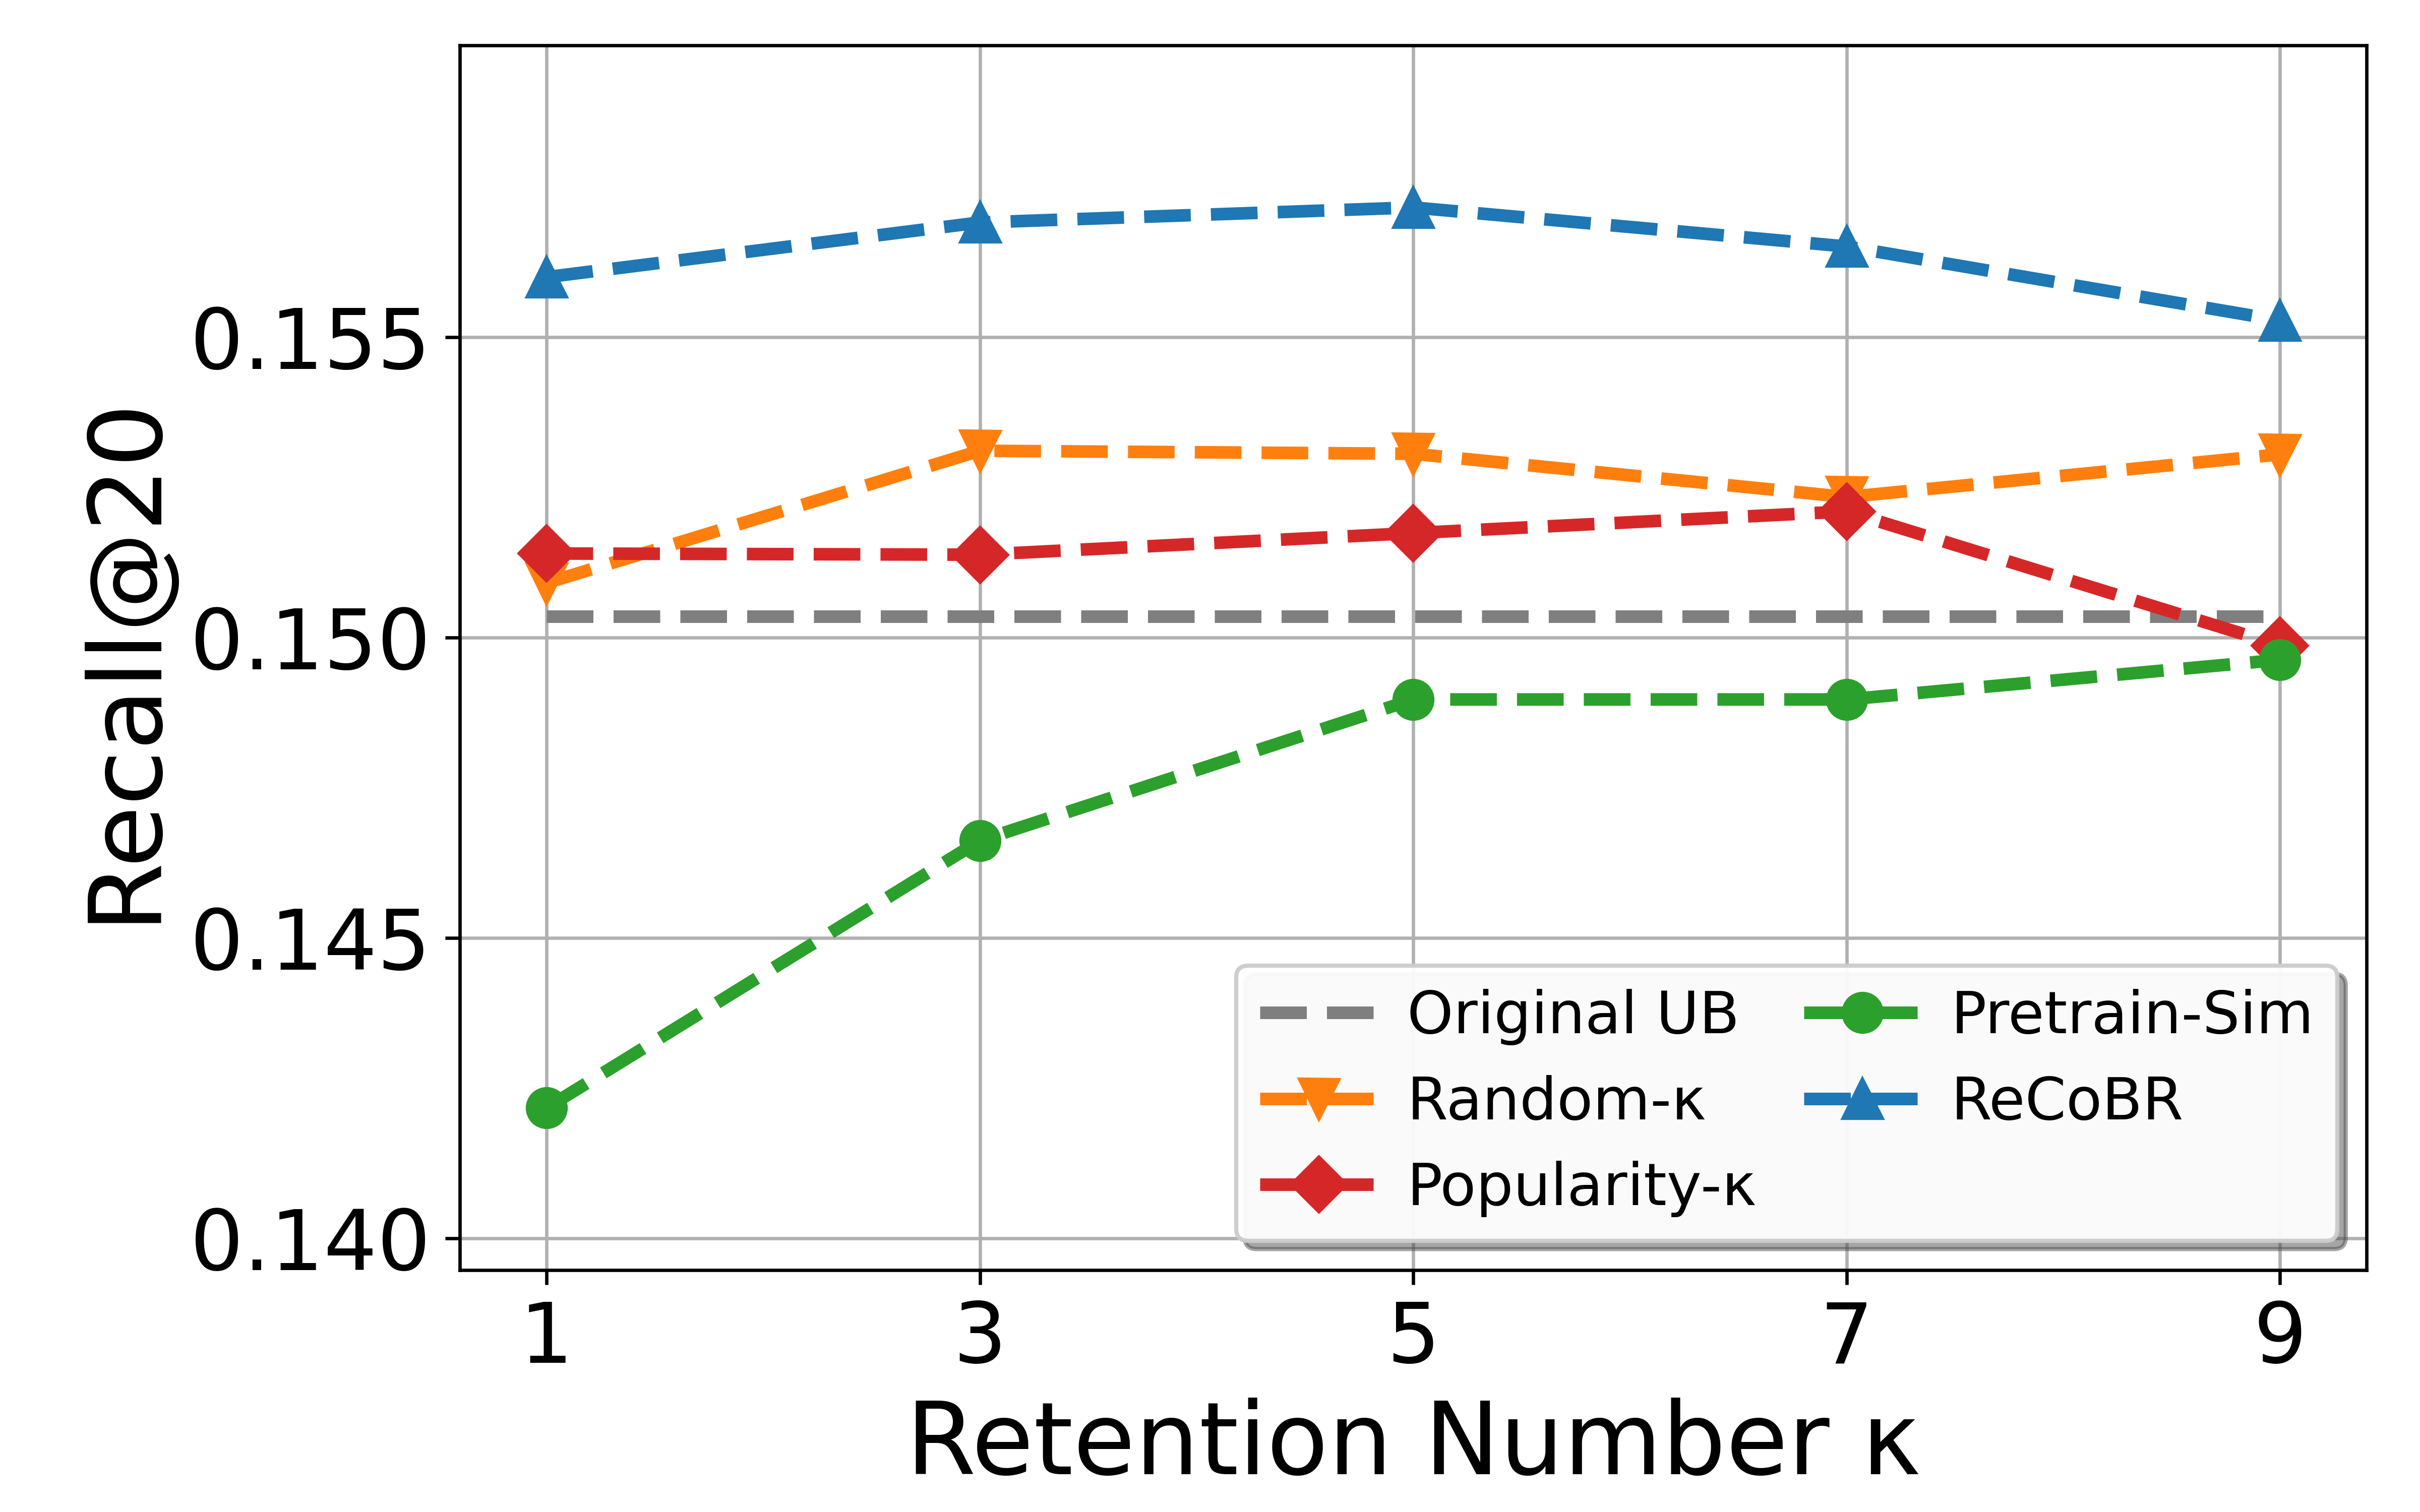
\includegraphics[width=0.46\columnwidth]
        {Figures/m1recall20.png} &
        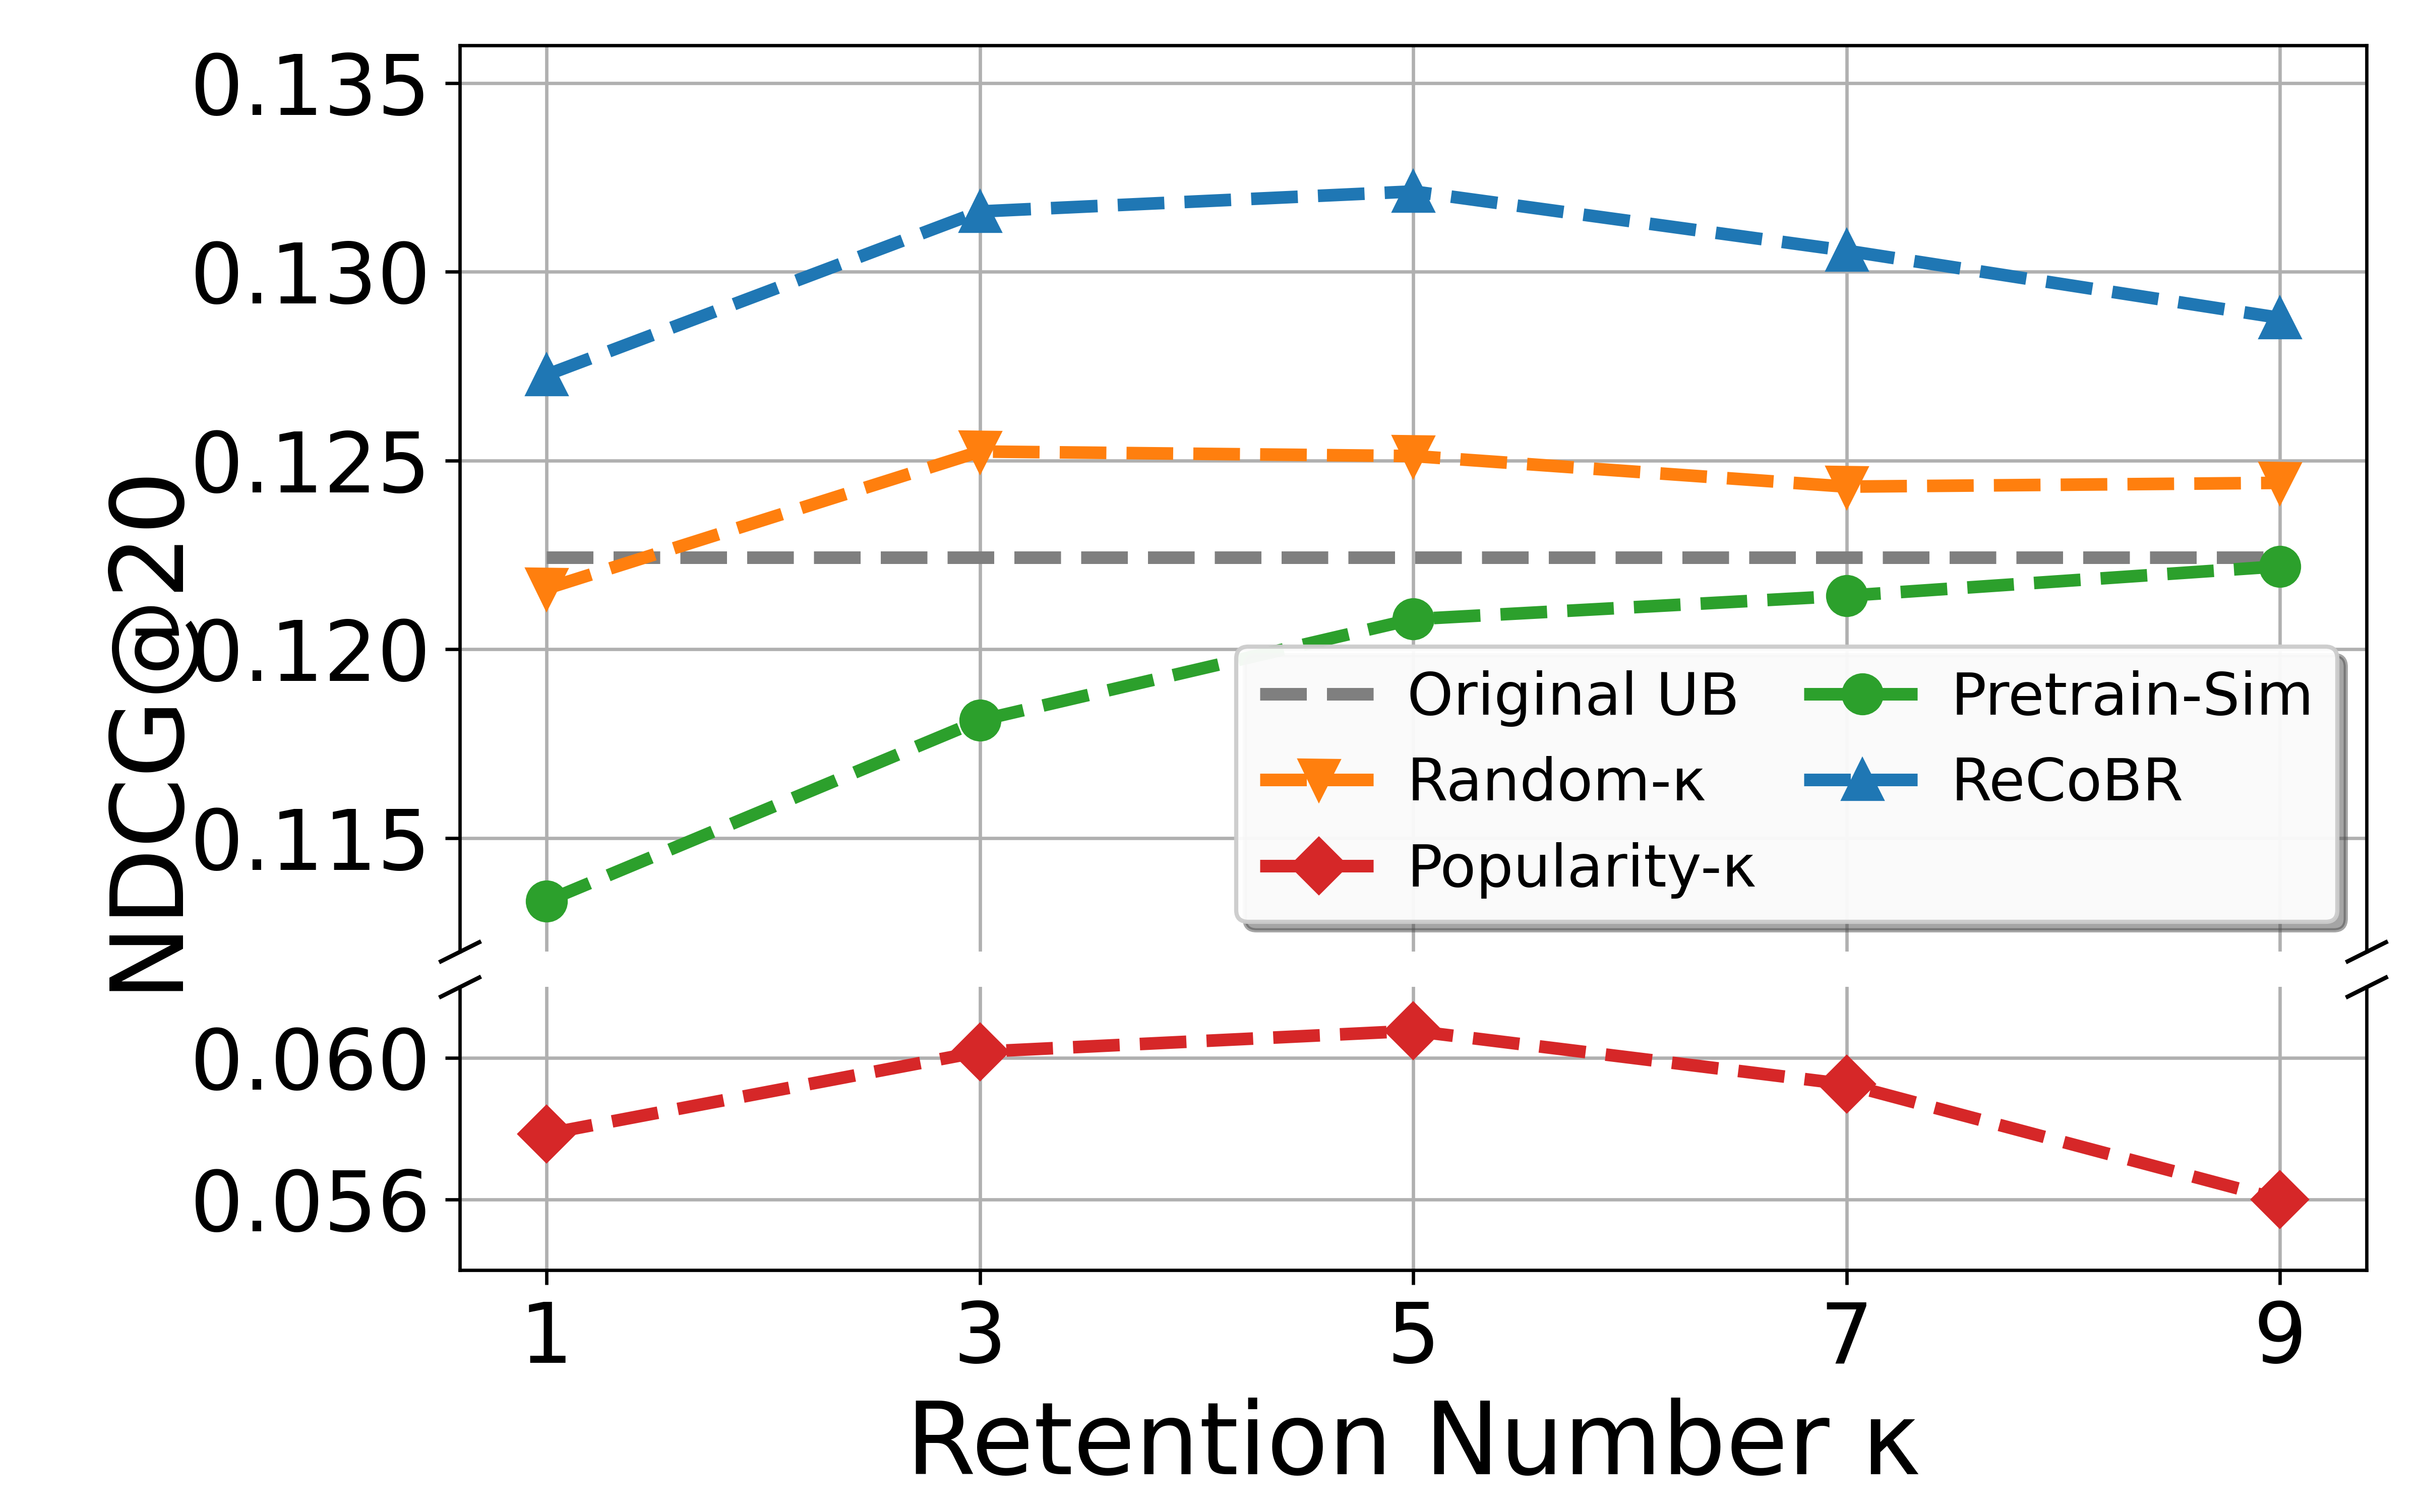
\includegraphics[width=0.46\columnwidth]
        {Figures/m1ndcg20.png} \\
        (a) & (b)
    \end{tabular}

    \caption{Interaction selection on iFashion using Recall@20
    and NDCG@20. The horizontal-axis variable $K$ denotes the
    per-user retention limit $\kappa$.}
    \label{fig:interaction-selection}
\end{figure}

\subsection{In-depth Analysis}

\begin{figure}[!t]
    \centering
    \begin{tabular}{@{}cc@{}}
        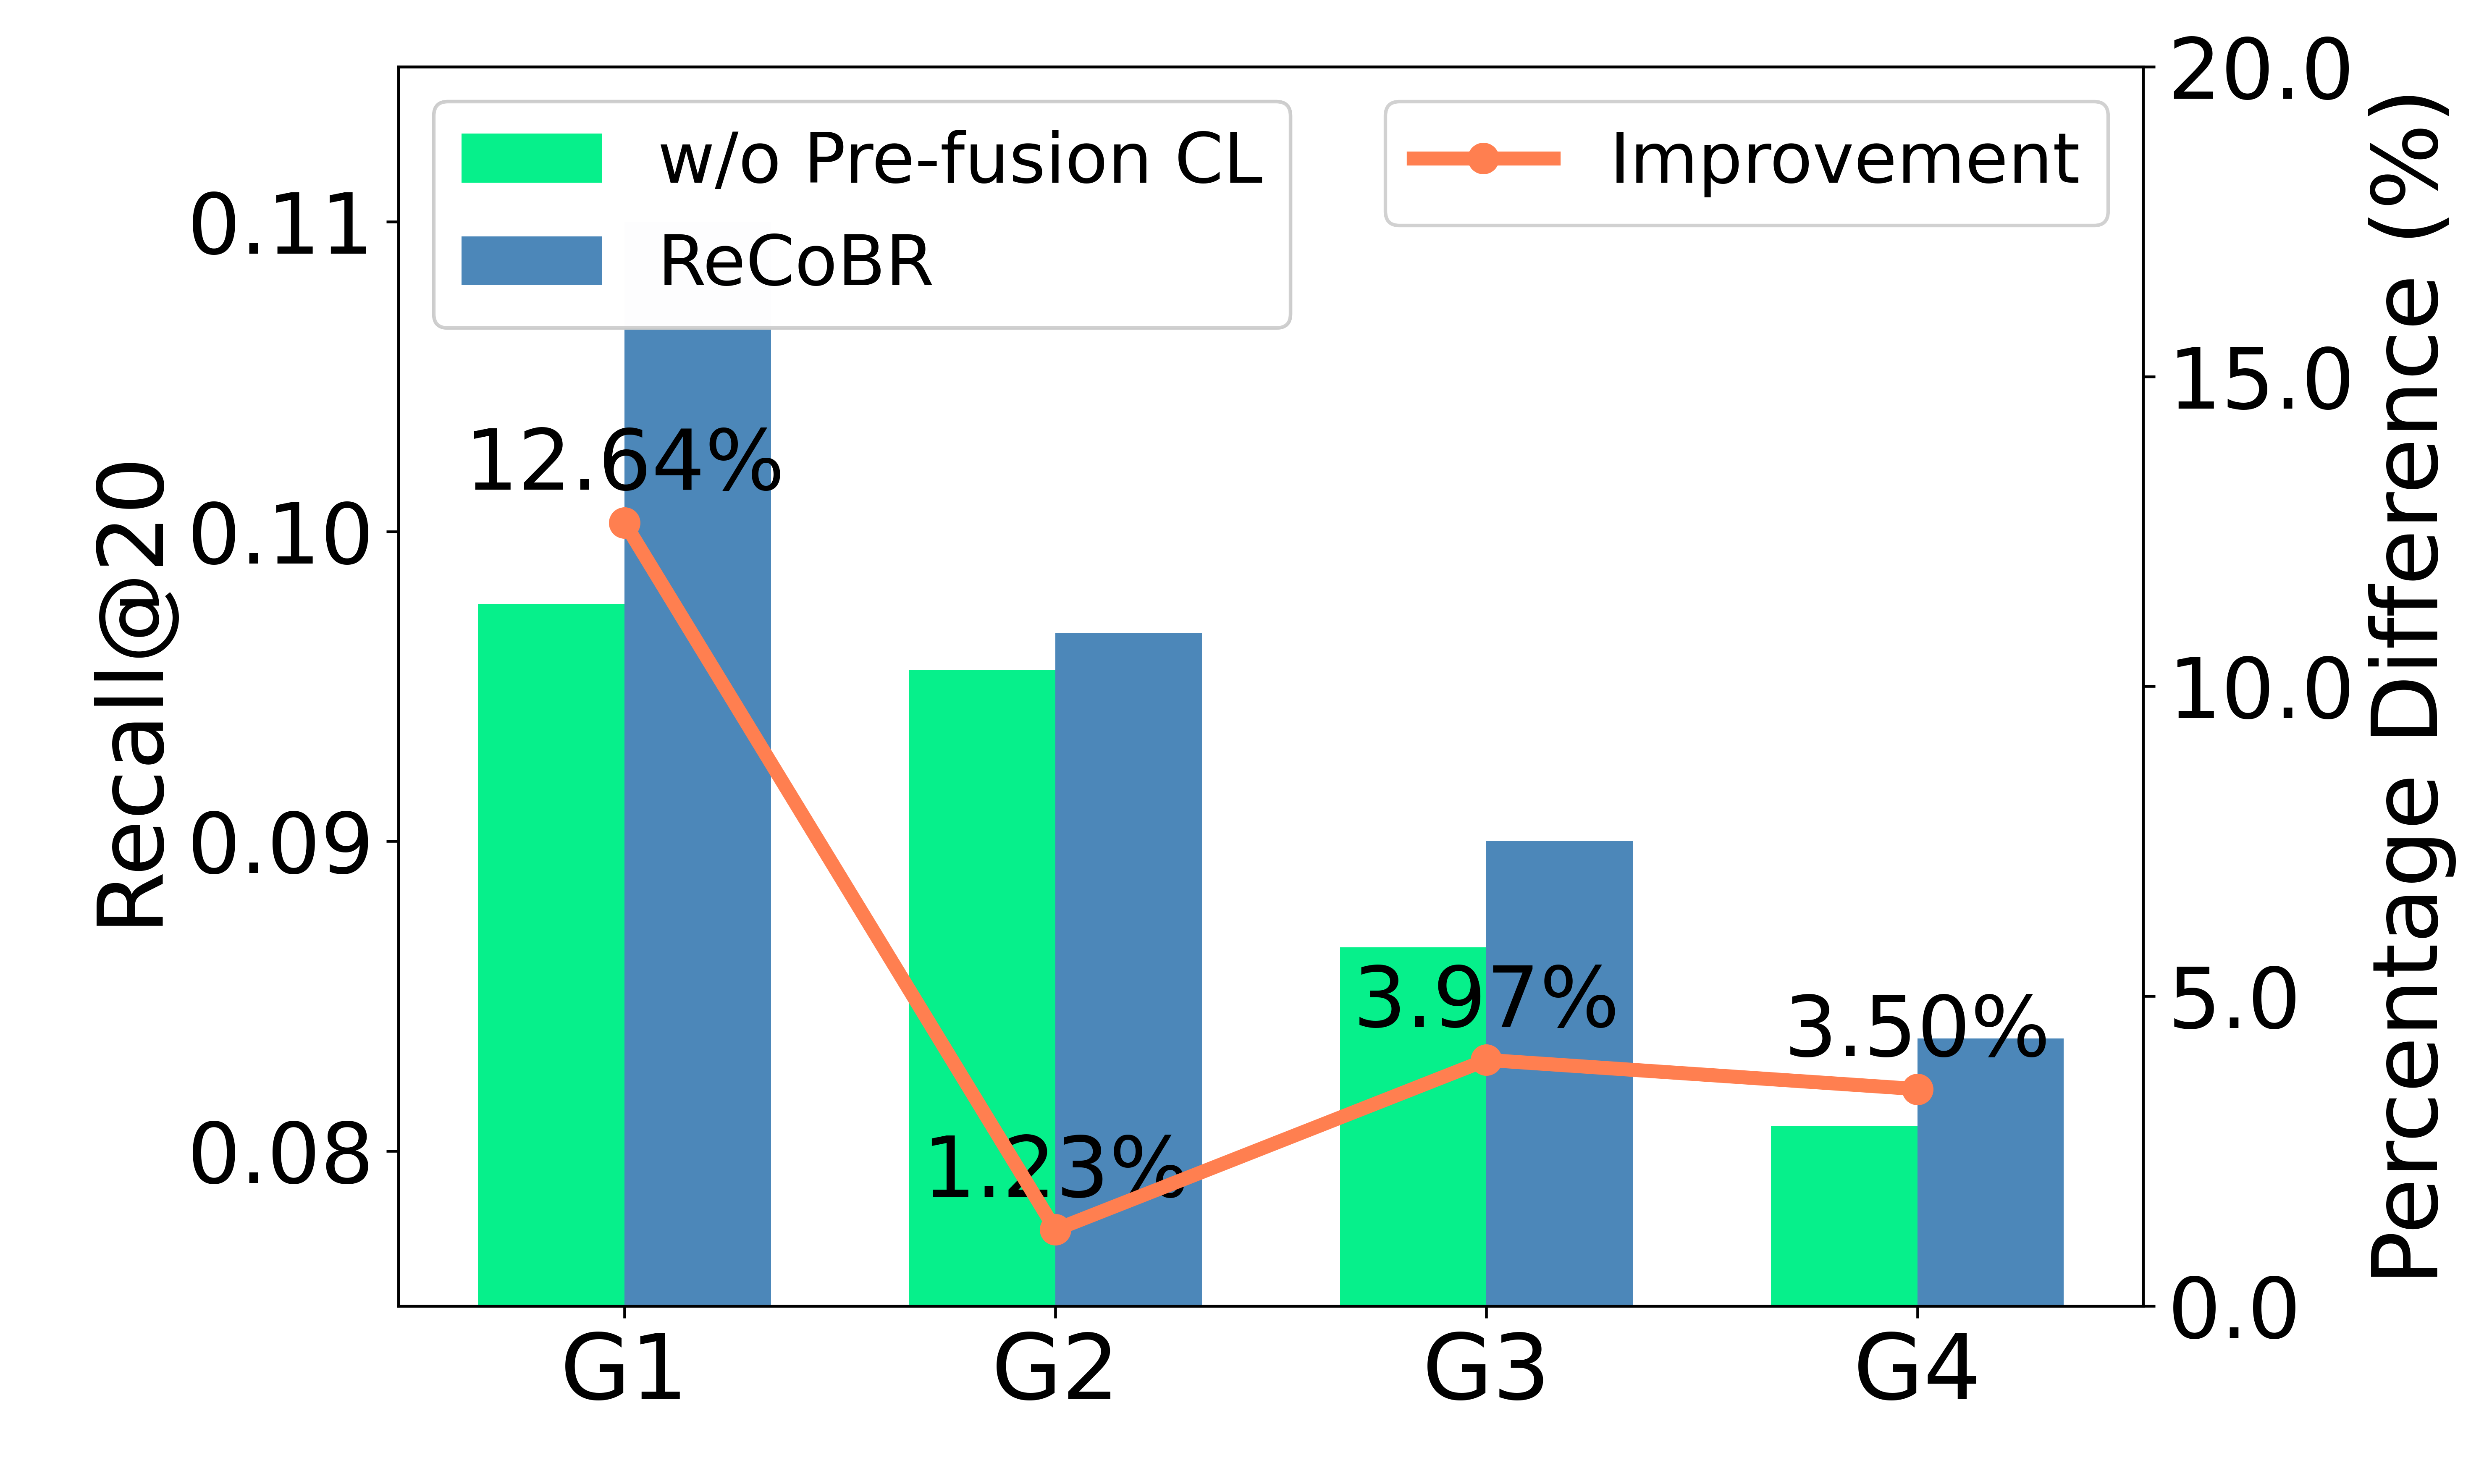
\includegraphics[width=0.46\columnwidth]
        {Figures/m2recall20.png} &
        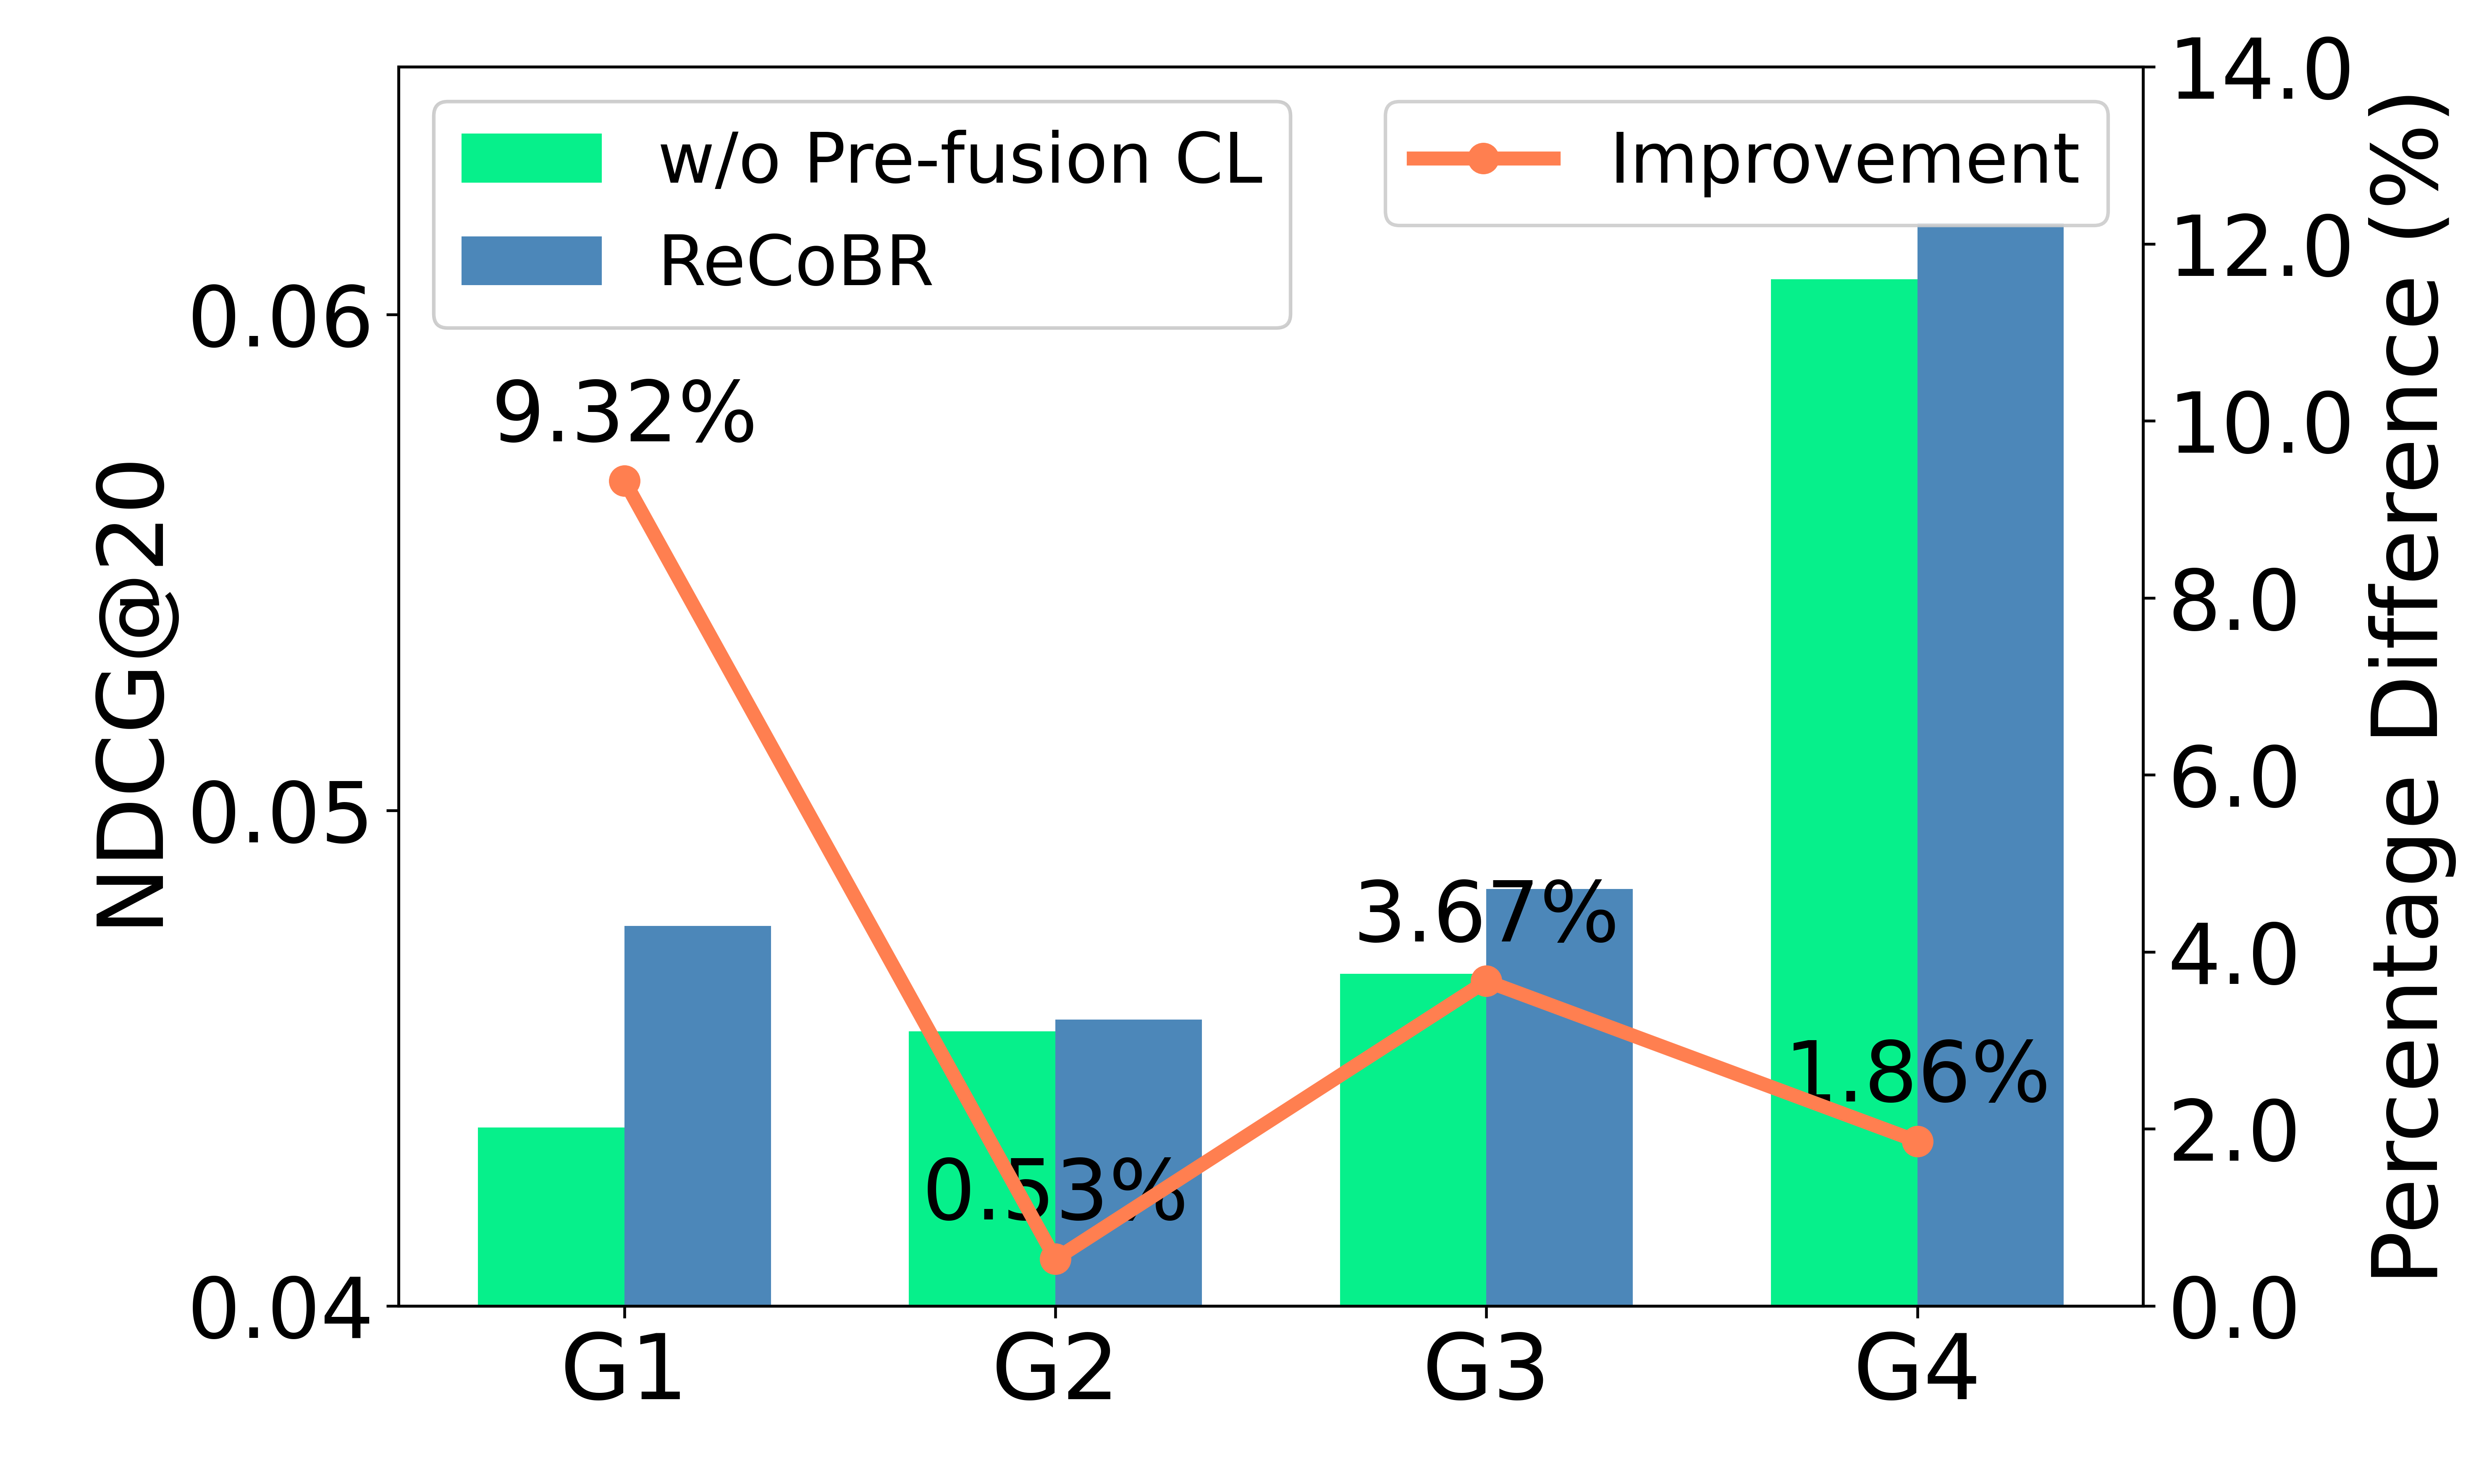
\includegraphics[width=0.46\columnwidth]
        {Figures/m2ndcg20.png} \\
        (a) & (b)
    \end{tabular}

    \caption{ReCoBR versus w/o CCL on NetEase using Recall@20
    and NDCG@20, both retaining PDGR.
    Users are sorted by increasing training U-B interaction counts
    and divided into four equally sized groups (G1--G4). Lines
    show relative improvements over w/o CCL.}
    \label{fig:sparse-users}
\end{figure}

\begin{figure}[!b]
    \centering
    \begin{tabular}{@{}c@{\hspace{0.02\columnwidth}}c@{}}
        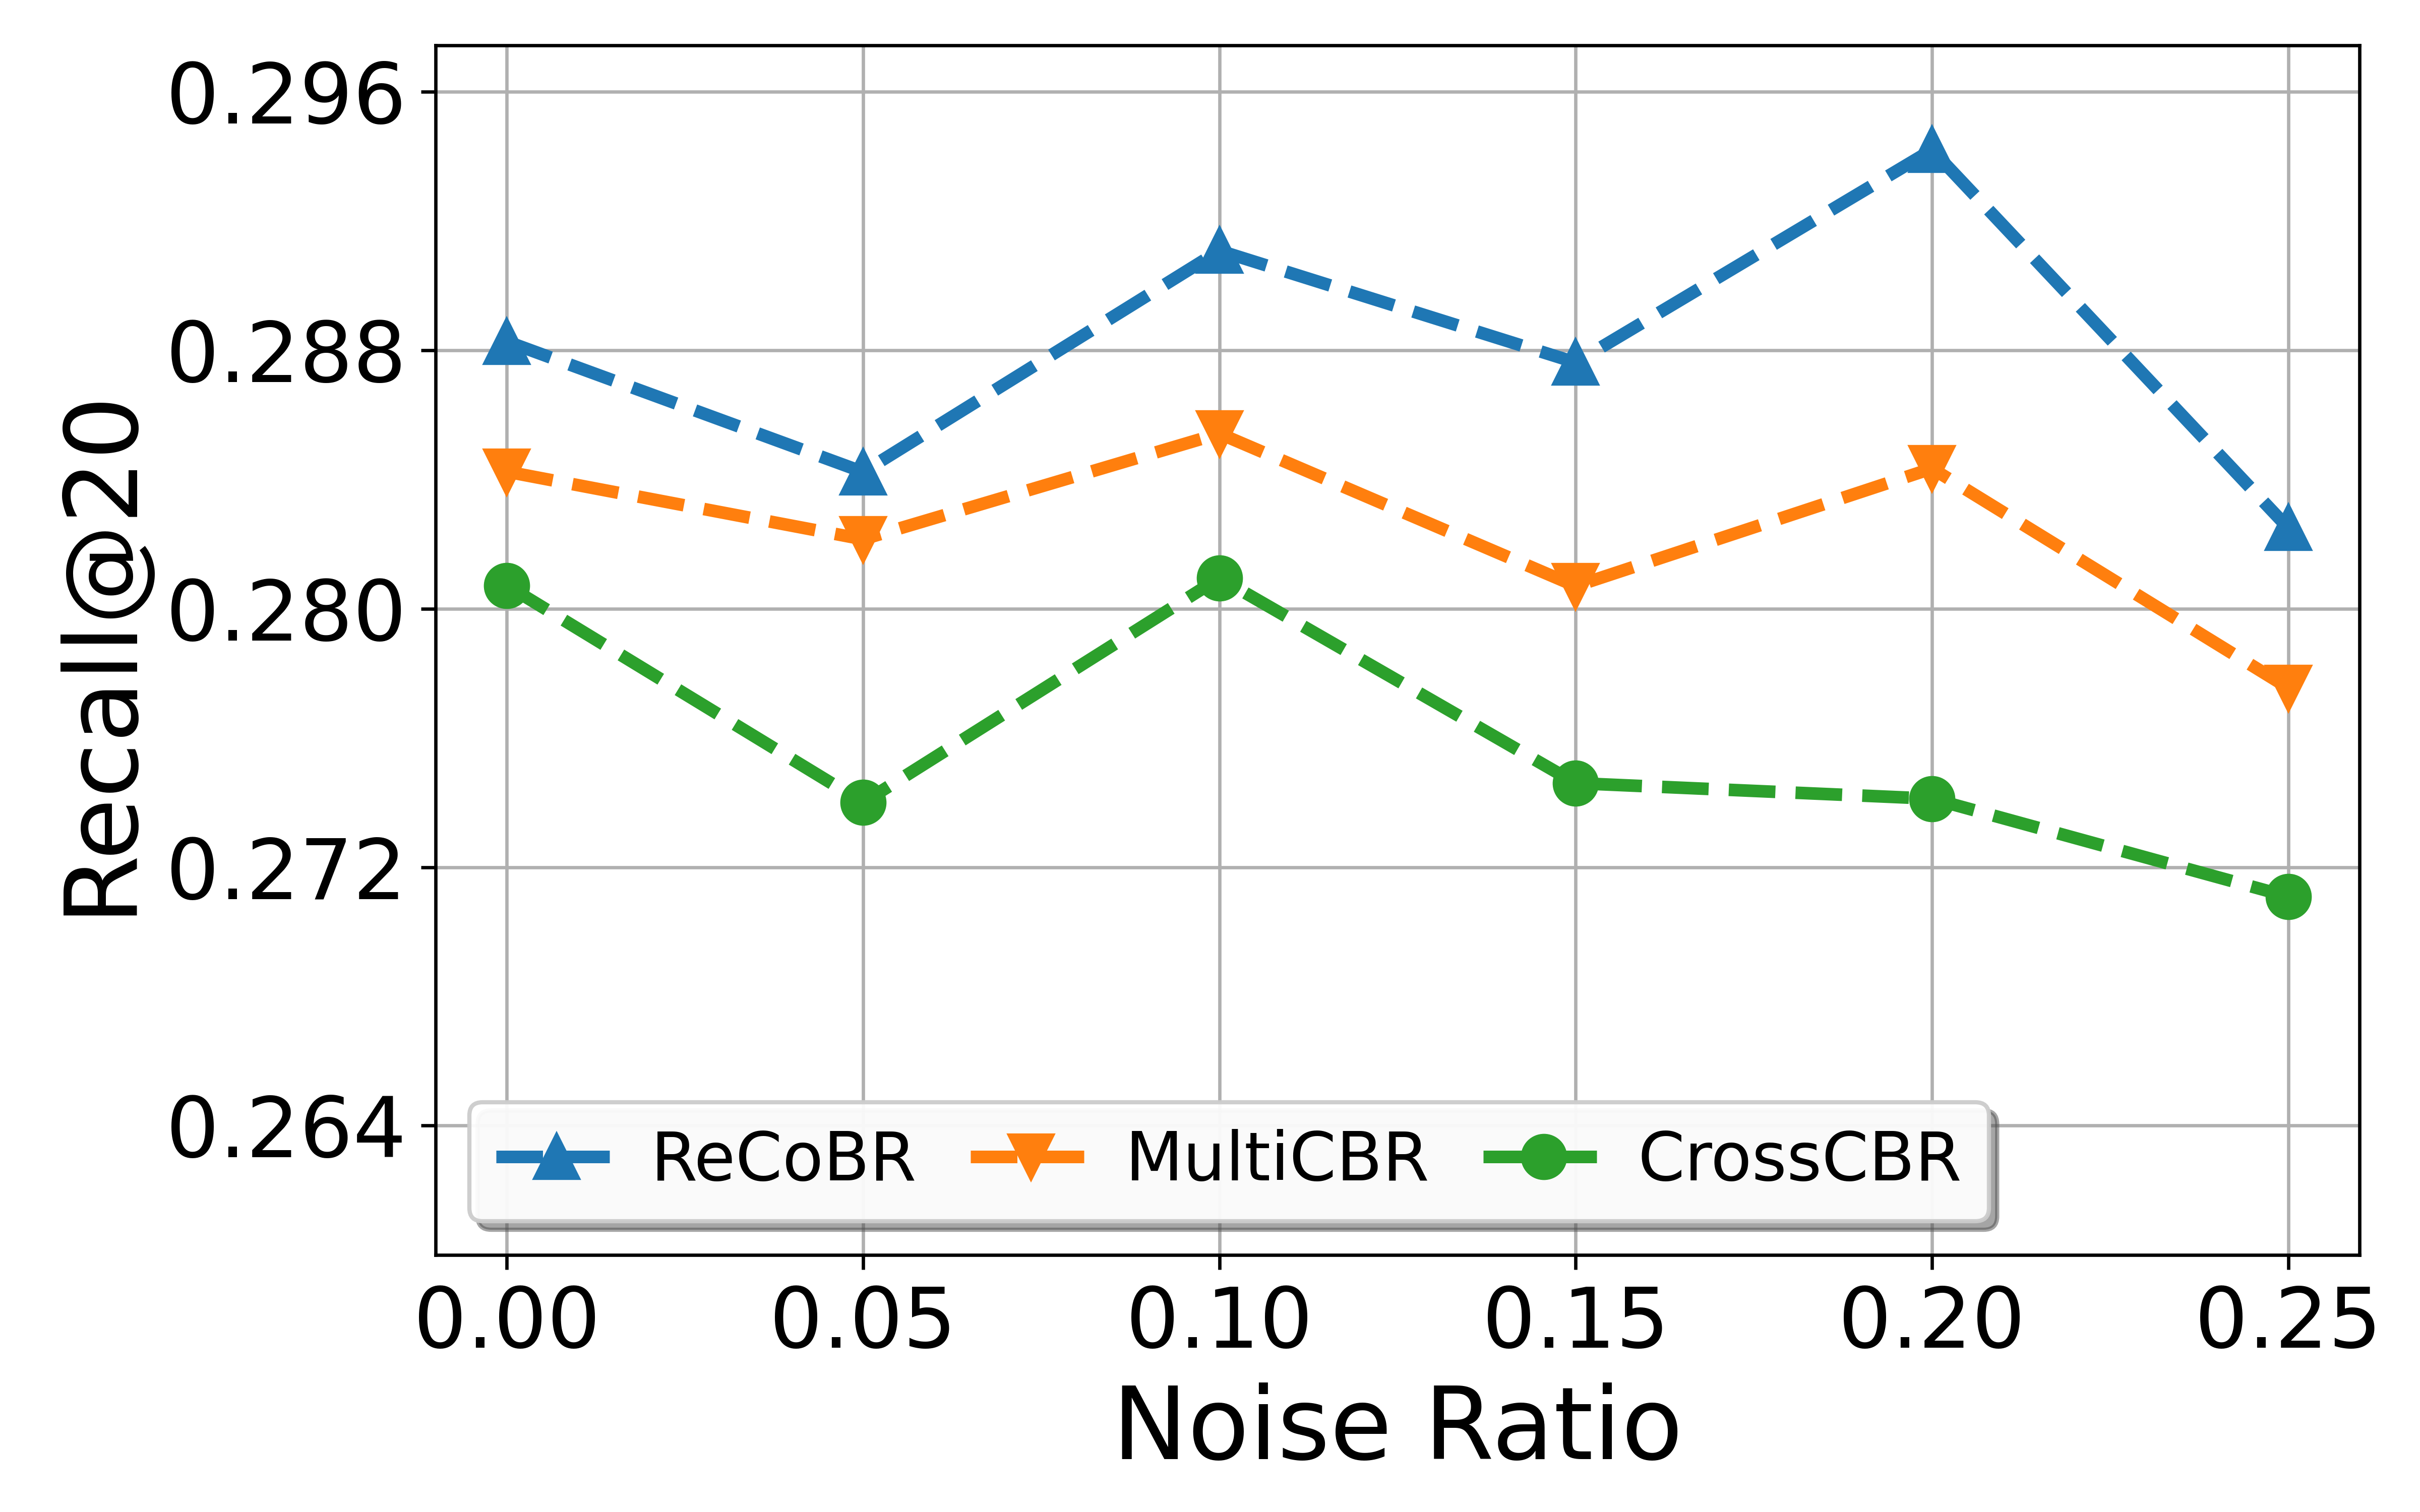
\includegraphics[width=0.48\columnwidth]{Figures/noise_youshu_r20.png} &
        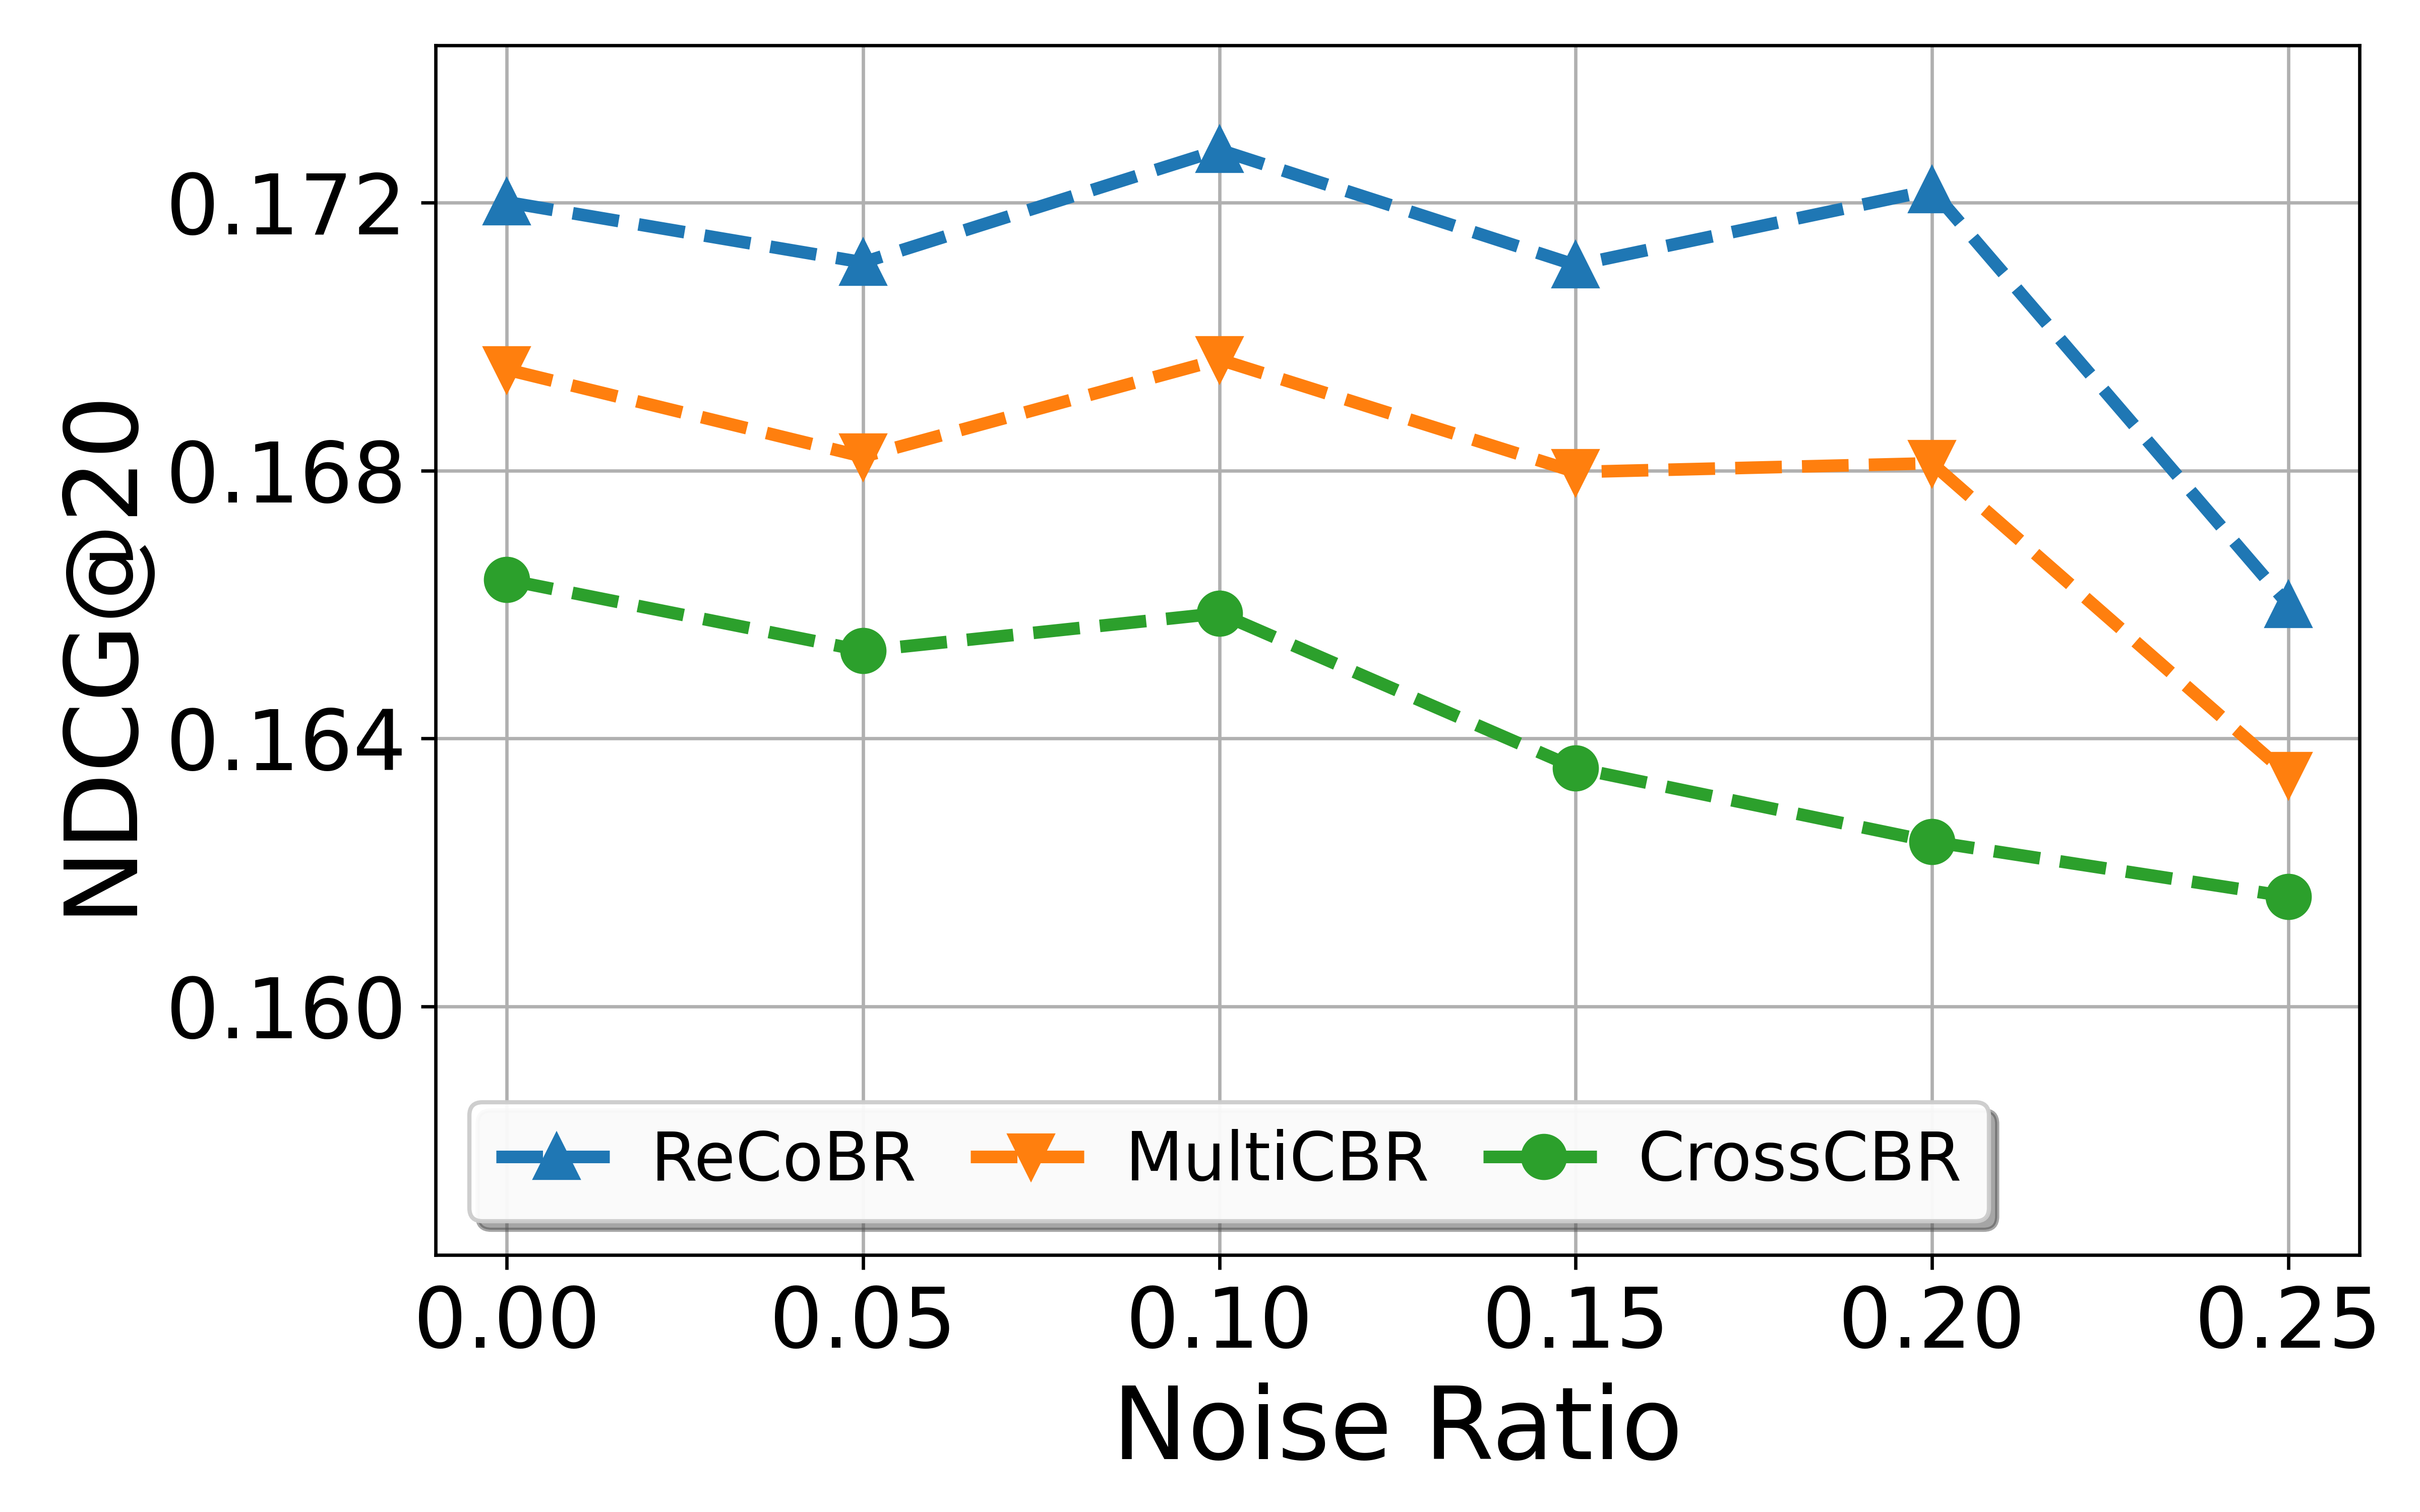
\includegraphics[width=0.48\columnwidth]{Figures/noise_youshu_n20.png} \\
        \multicolumn{2}{c}{(a) Youshu} \\
        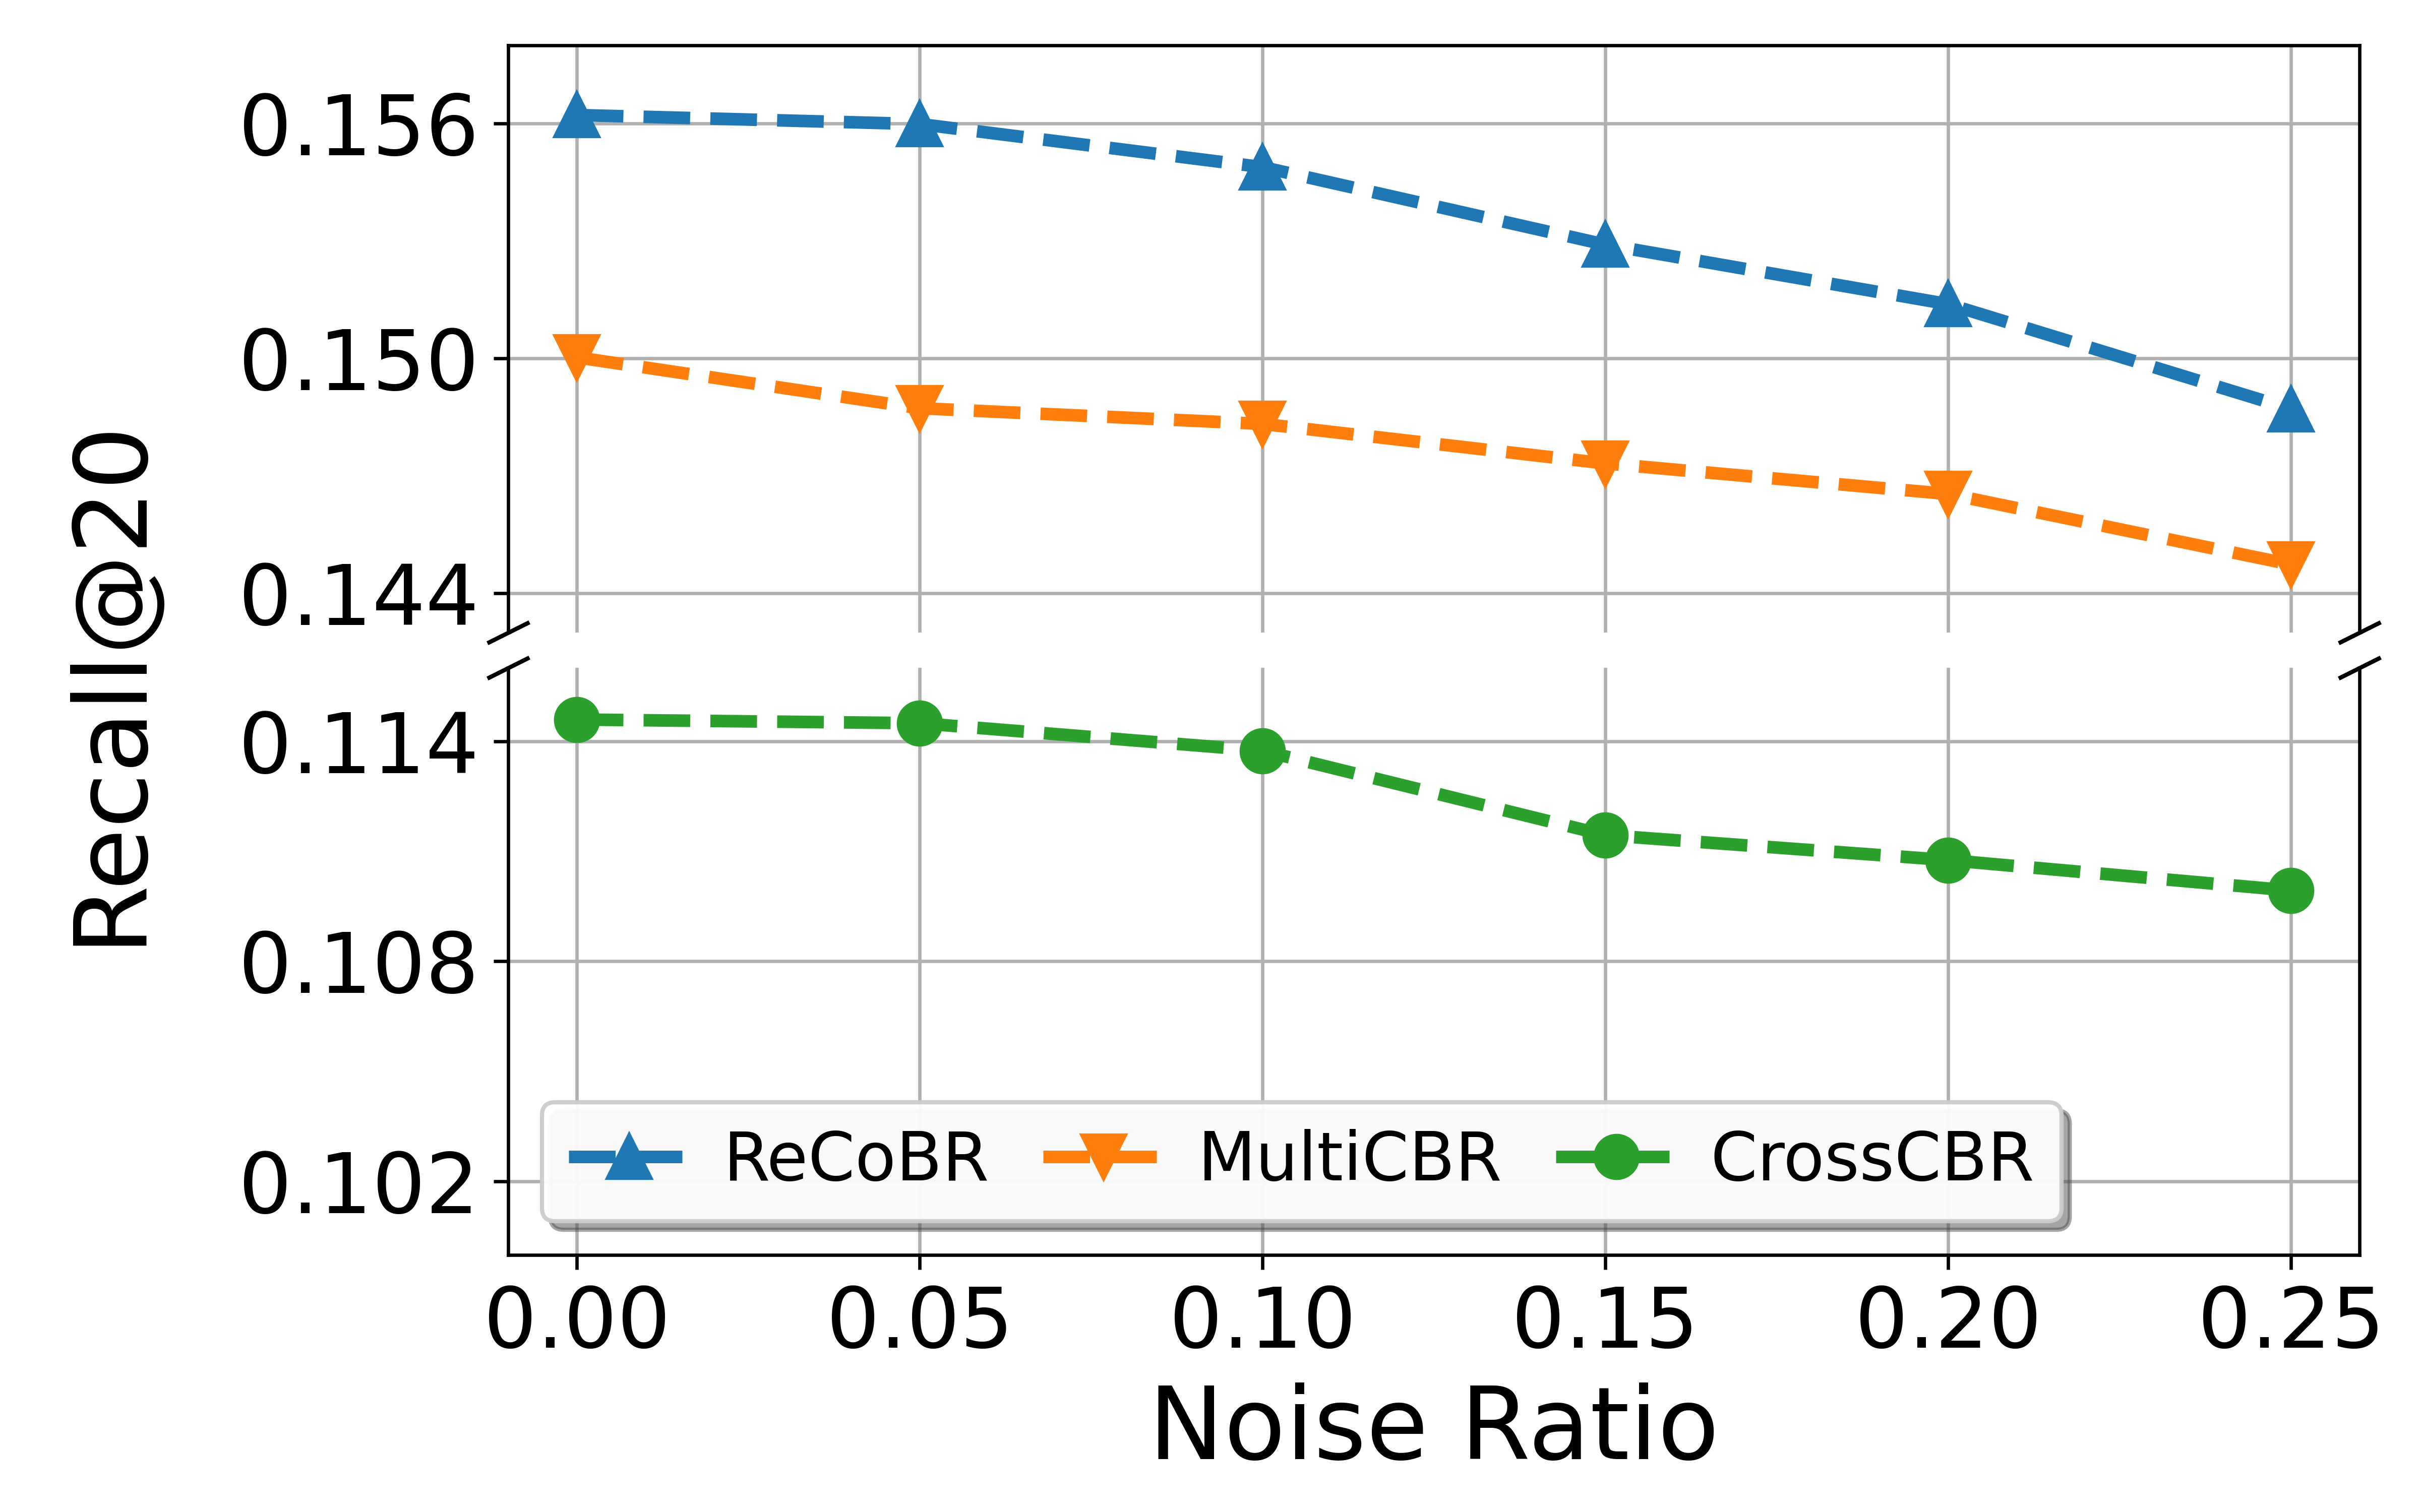
\includegraphics[width=0.48\columnwidth]{Figures/noise_ifashion_r20.png} &
        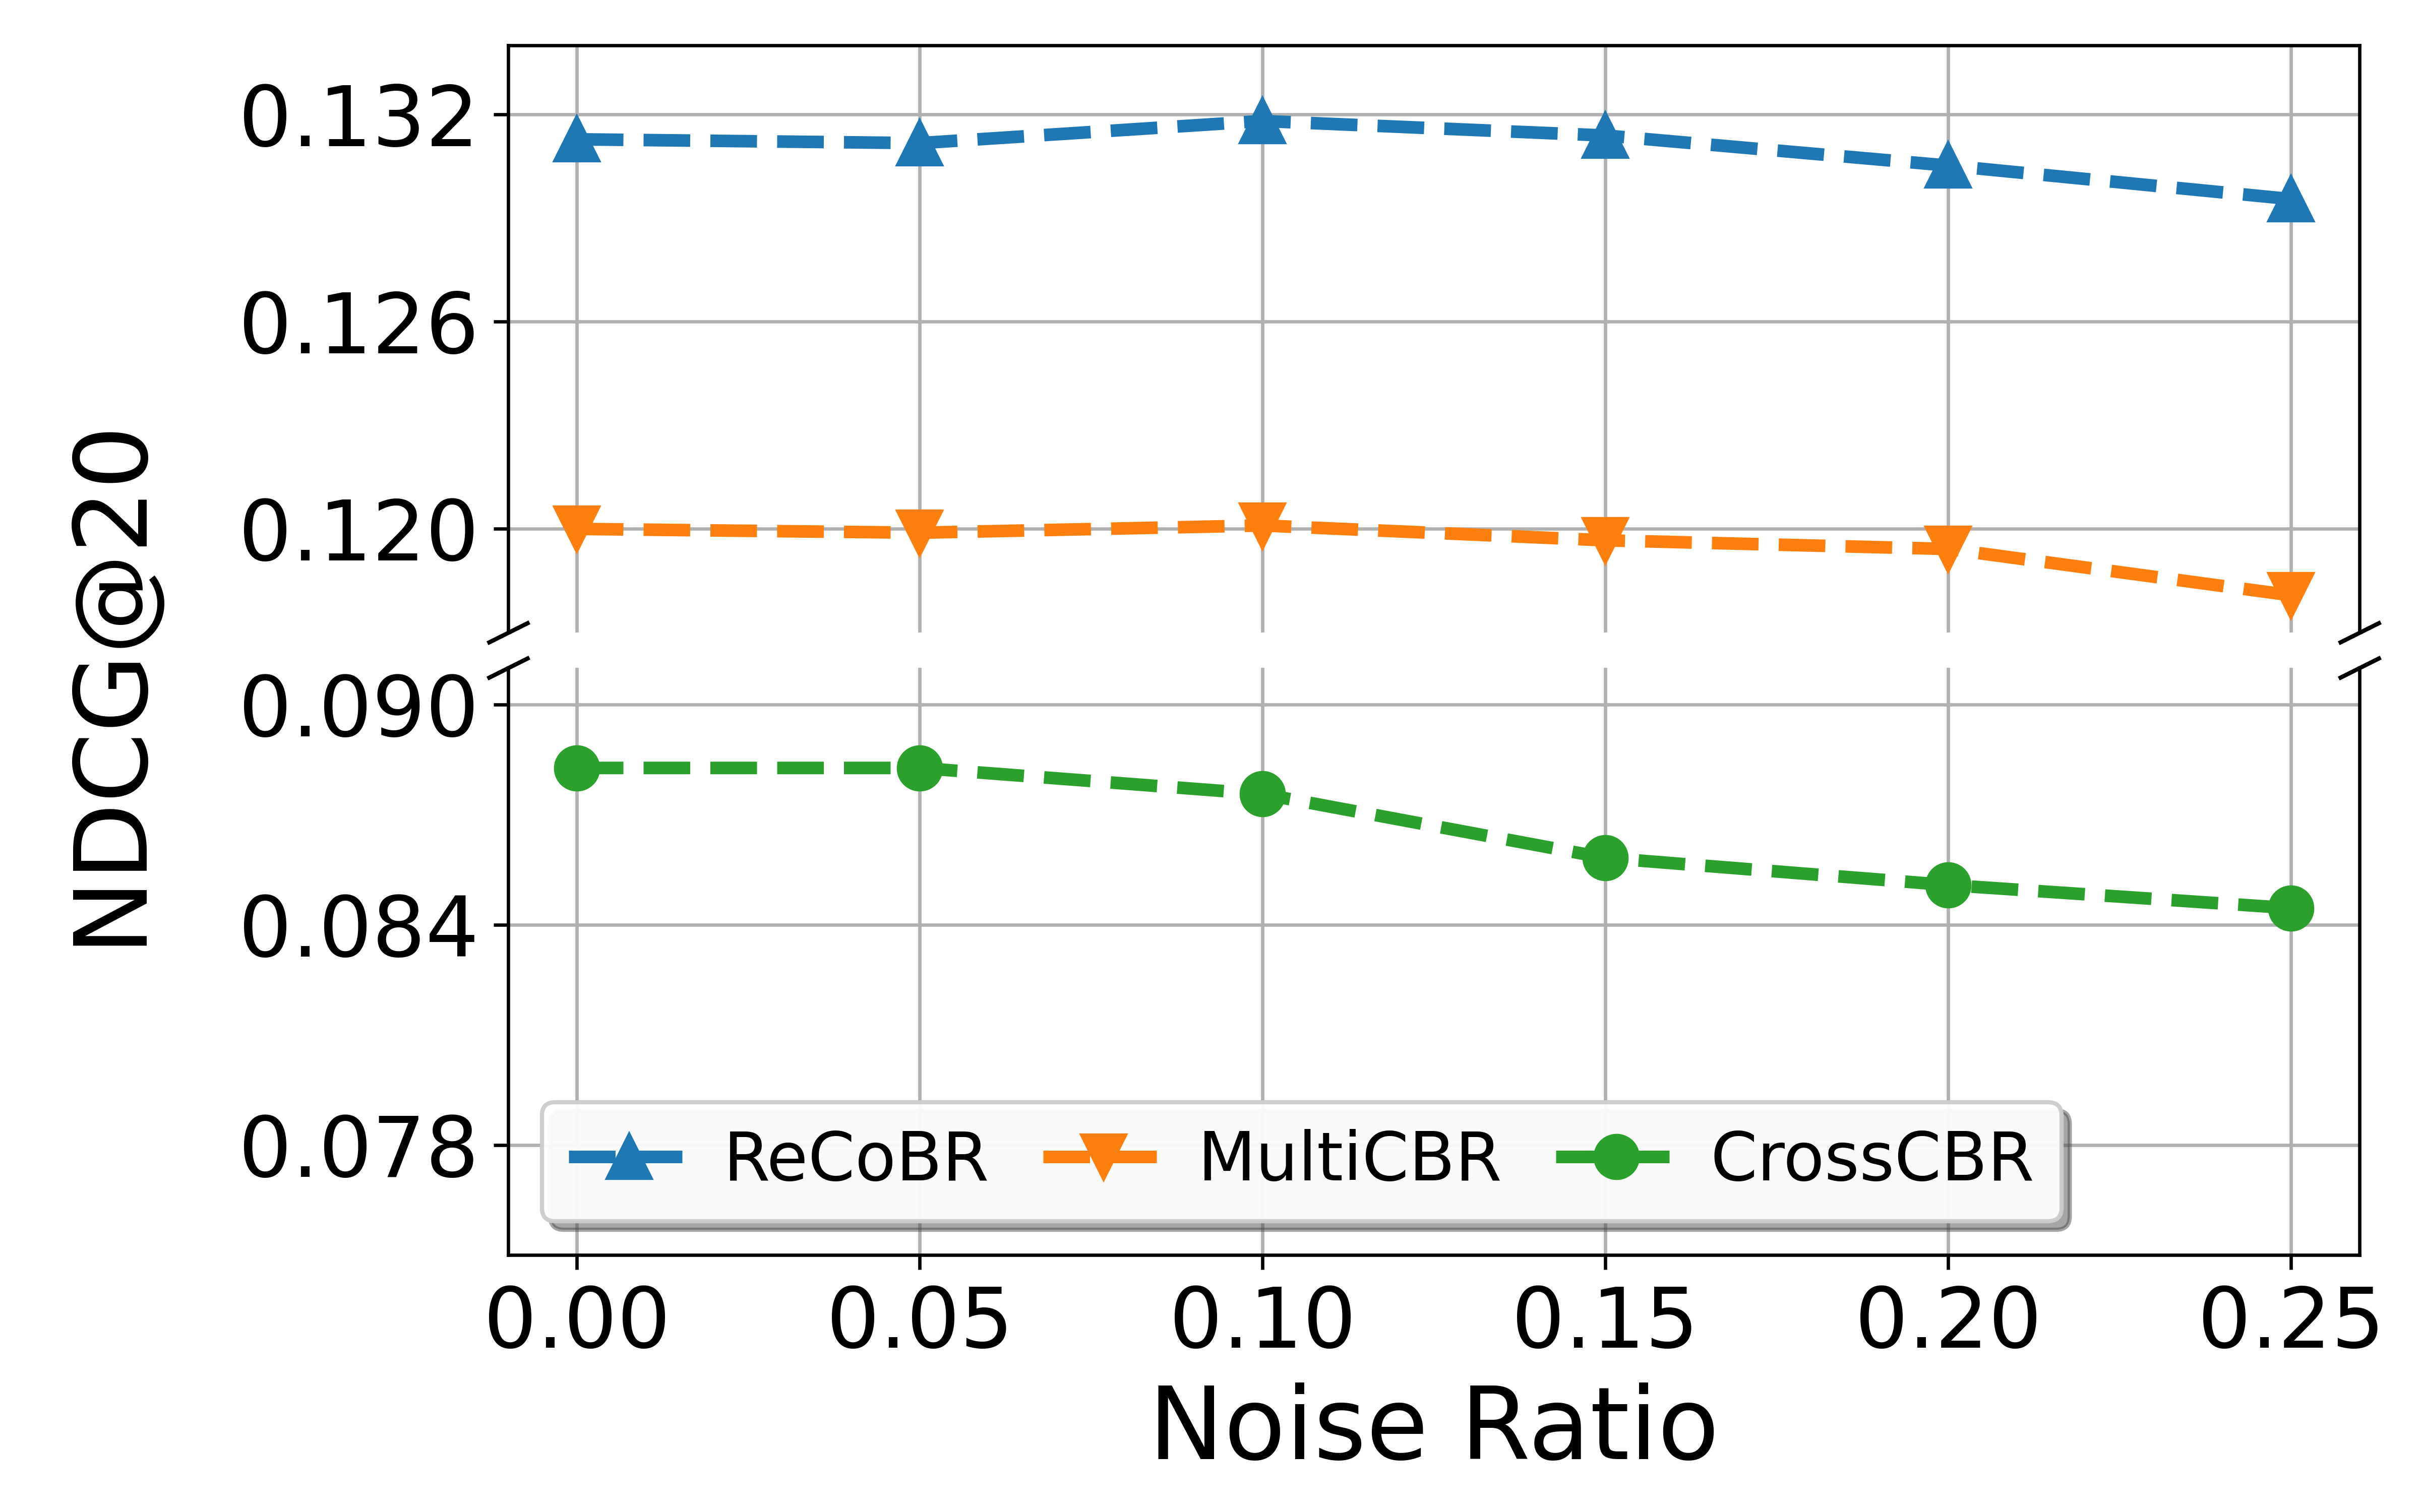
\includegraphics[width=0.48\columnwidth]{Figures/noise_ifashion_n20.png} \\
        \multicolumn{2}{c}{(b) iFashion} \\
        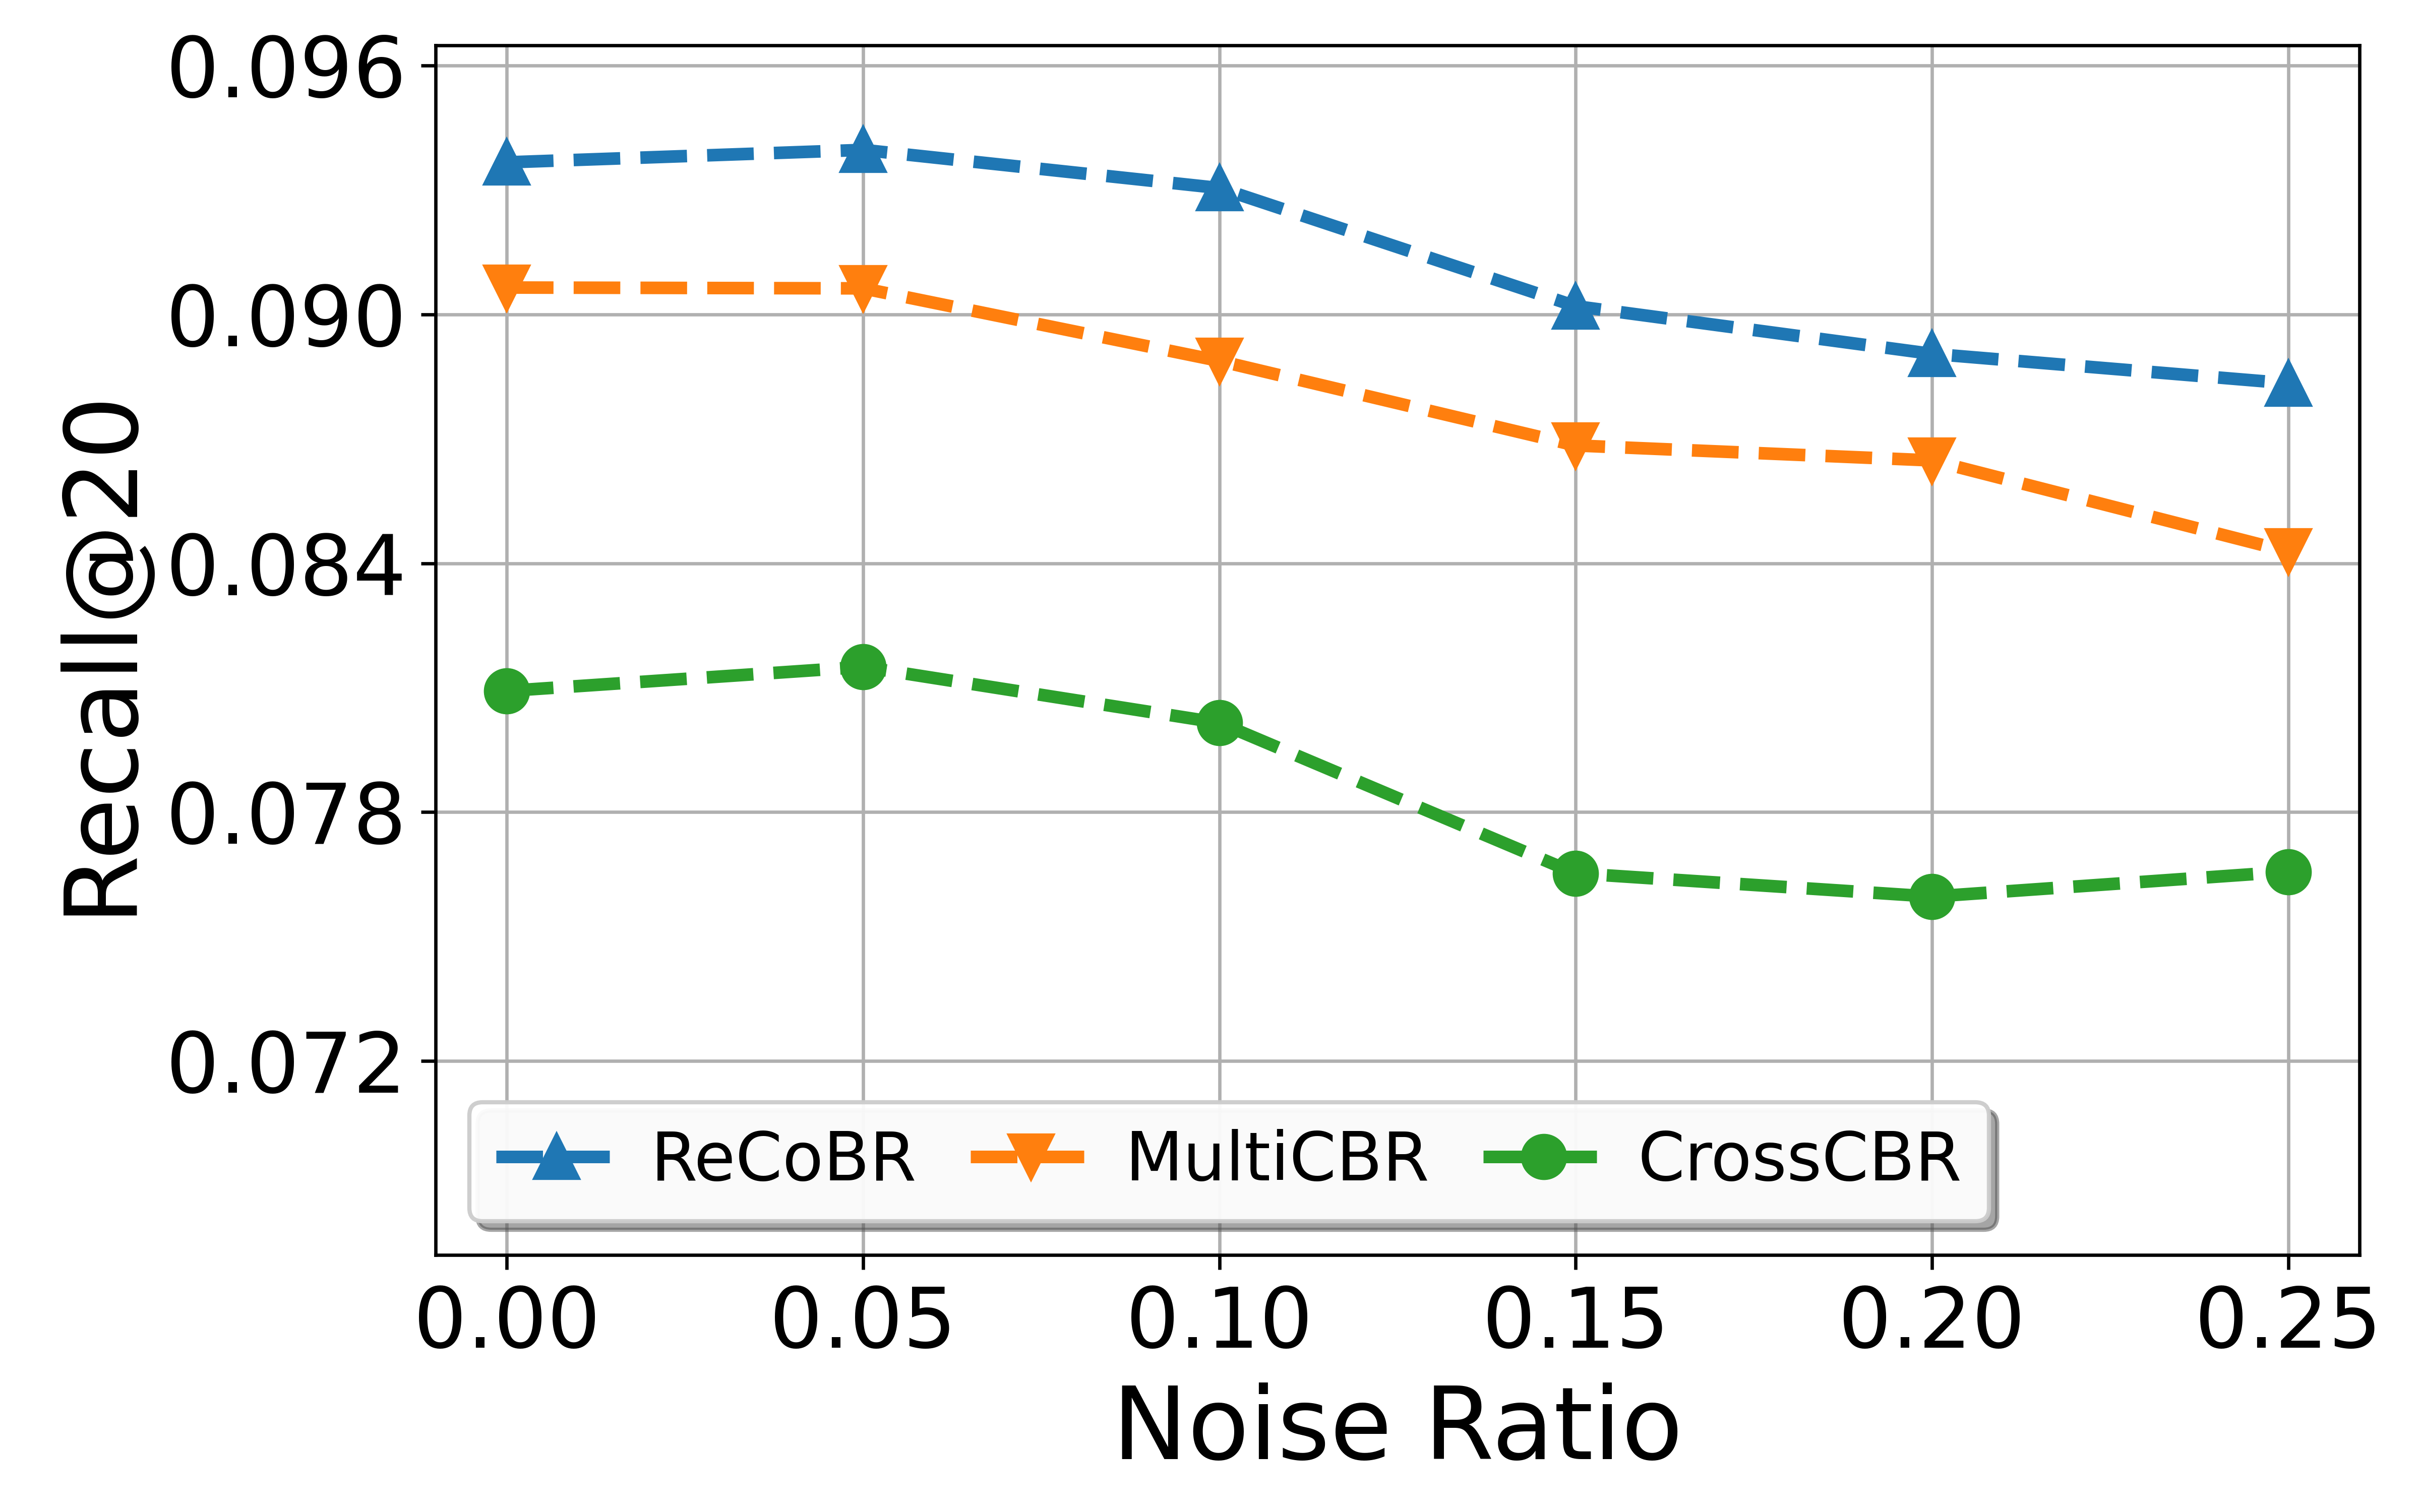
\includegraphics[width=0.48\columnwidth]{Figures/noise_netease_r20.png} &
        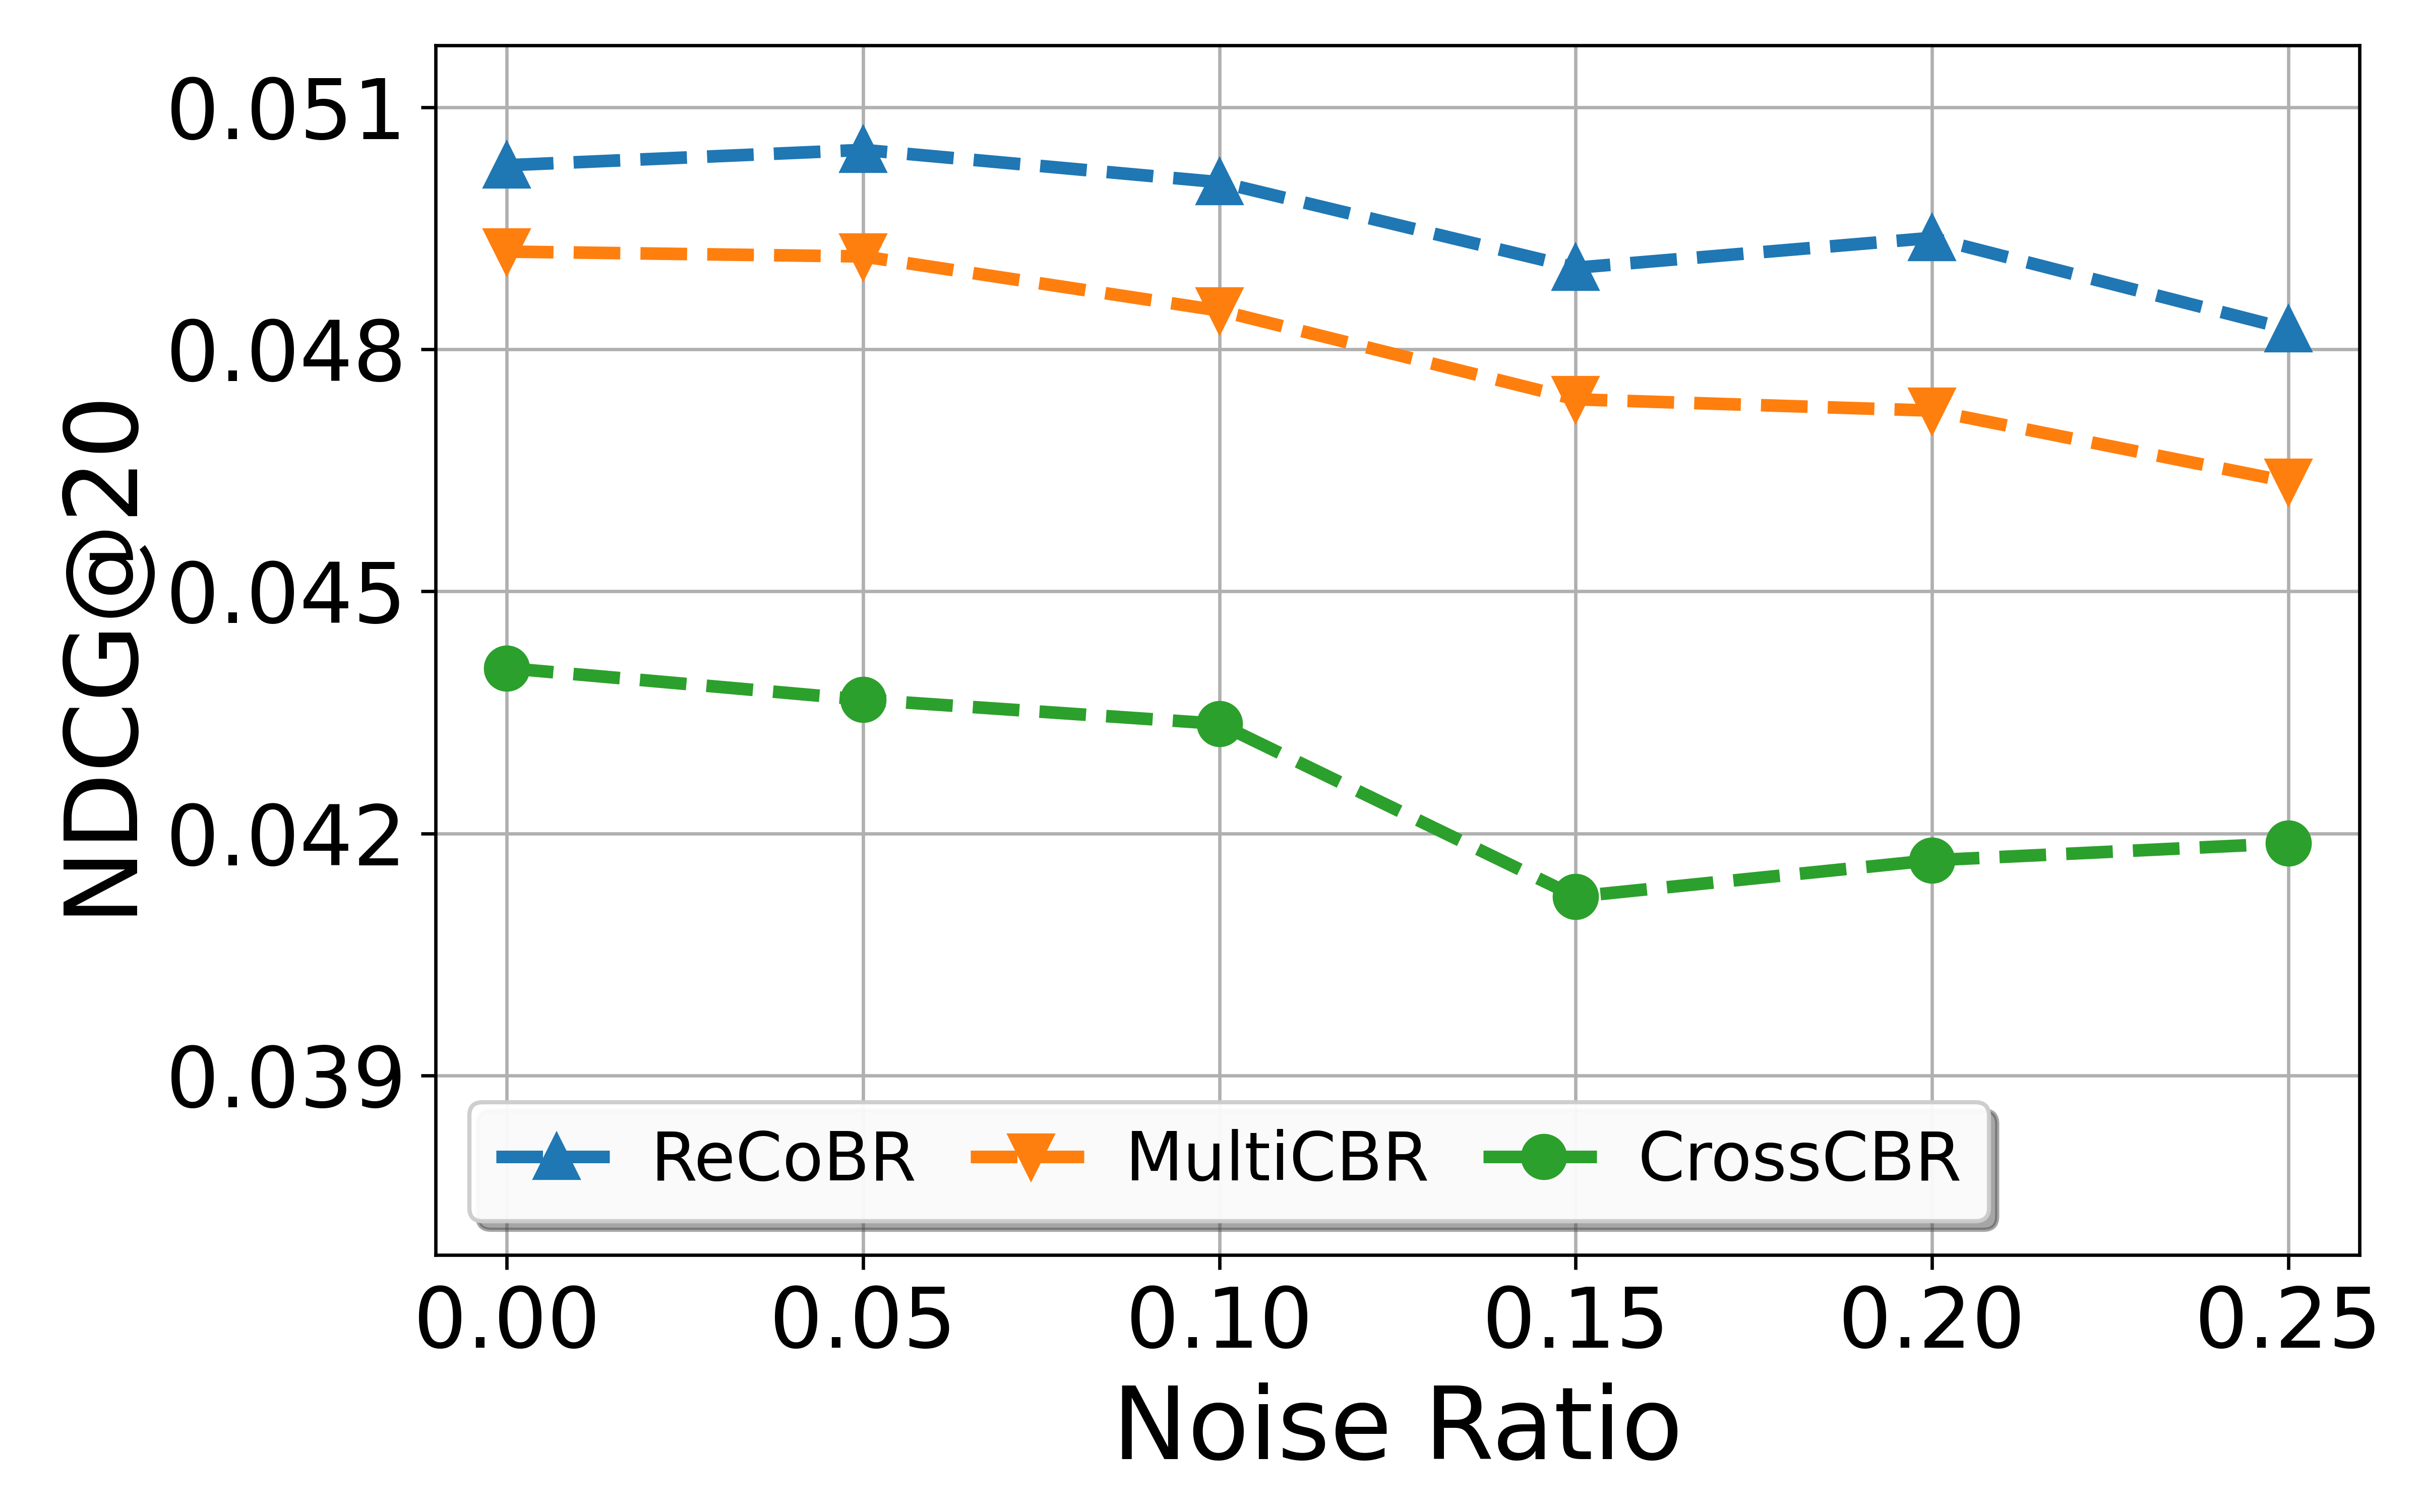
\includegraphics[width=0.48\columnwidth]{Figures/noise_netease_n20.png} \\
        \multicolumn{2}{c}{(c) NetEase}
    \end{tabular}
    \caption{Recall@20 and NDCG@20 under injected U-B graph noise on
    Youshu, iFashion, and NetEase. We add random edges at ratios from
    0\% to 25\% in 5\% increments relative to each user's original
    training interactions, retaining all original edges.}
    \label{fig:noise-robustness}
\end{figure}

\begin{figure*}[!t]
    \centering
    \begin{tabular}{@{}c@{\hspace{0.025\textwidth}}c@{\hspace{0.025\textwidth}}c@{}}
        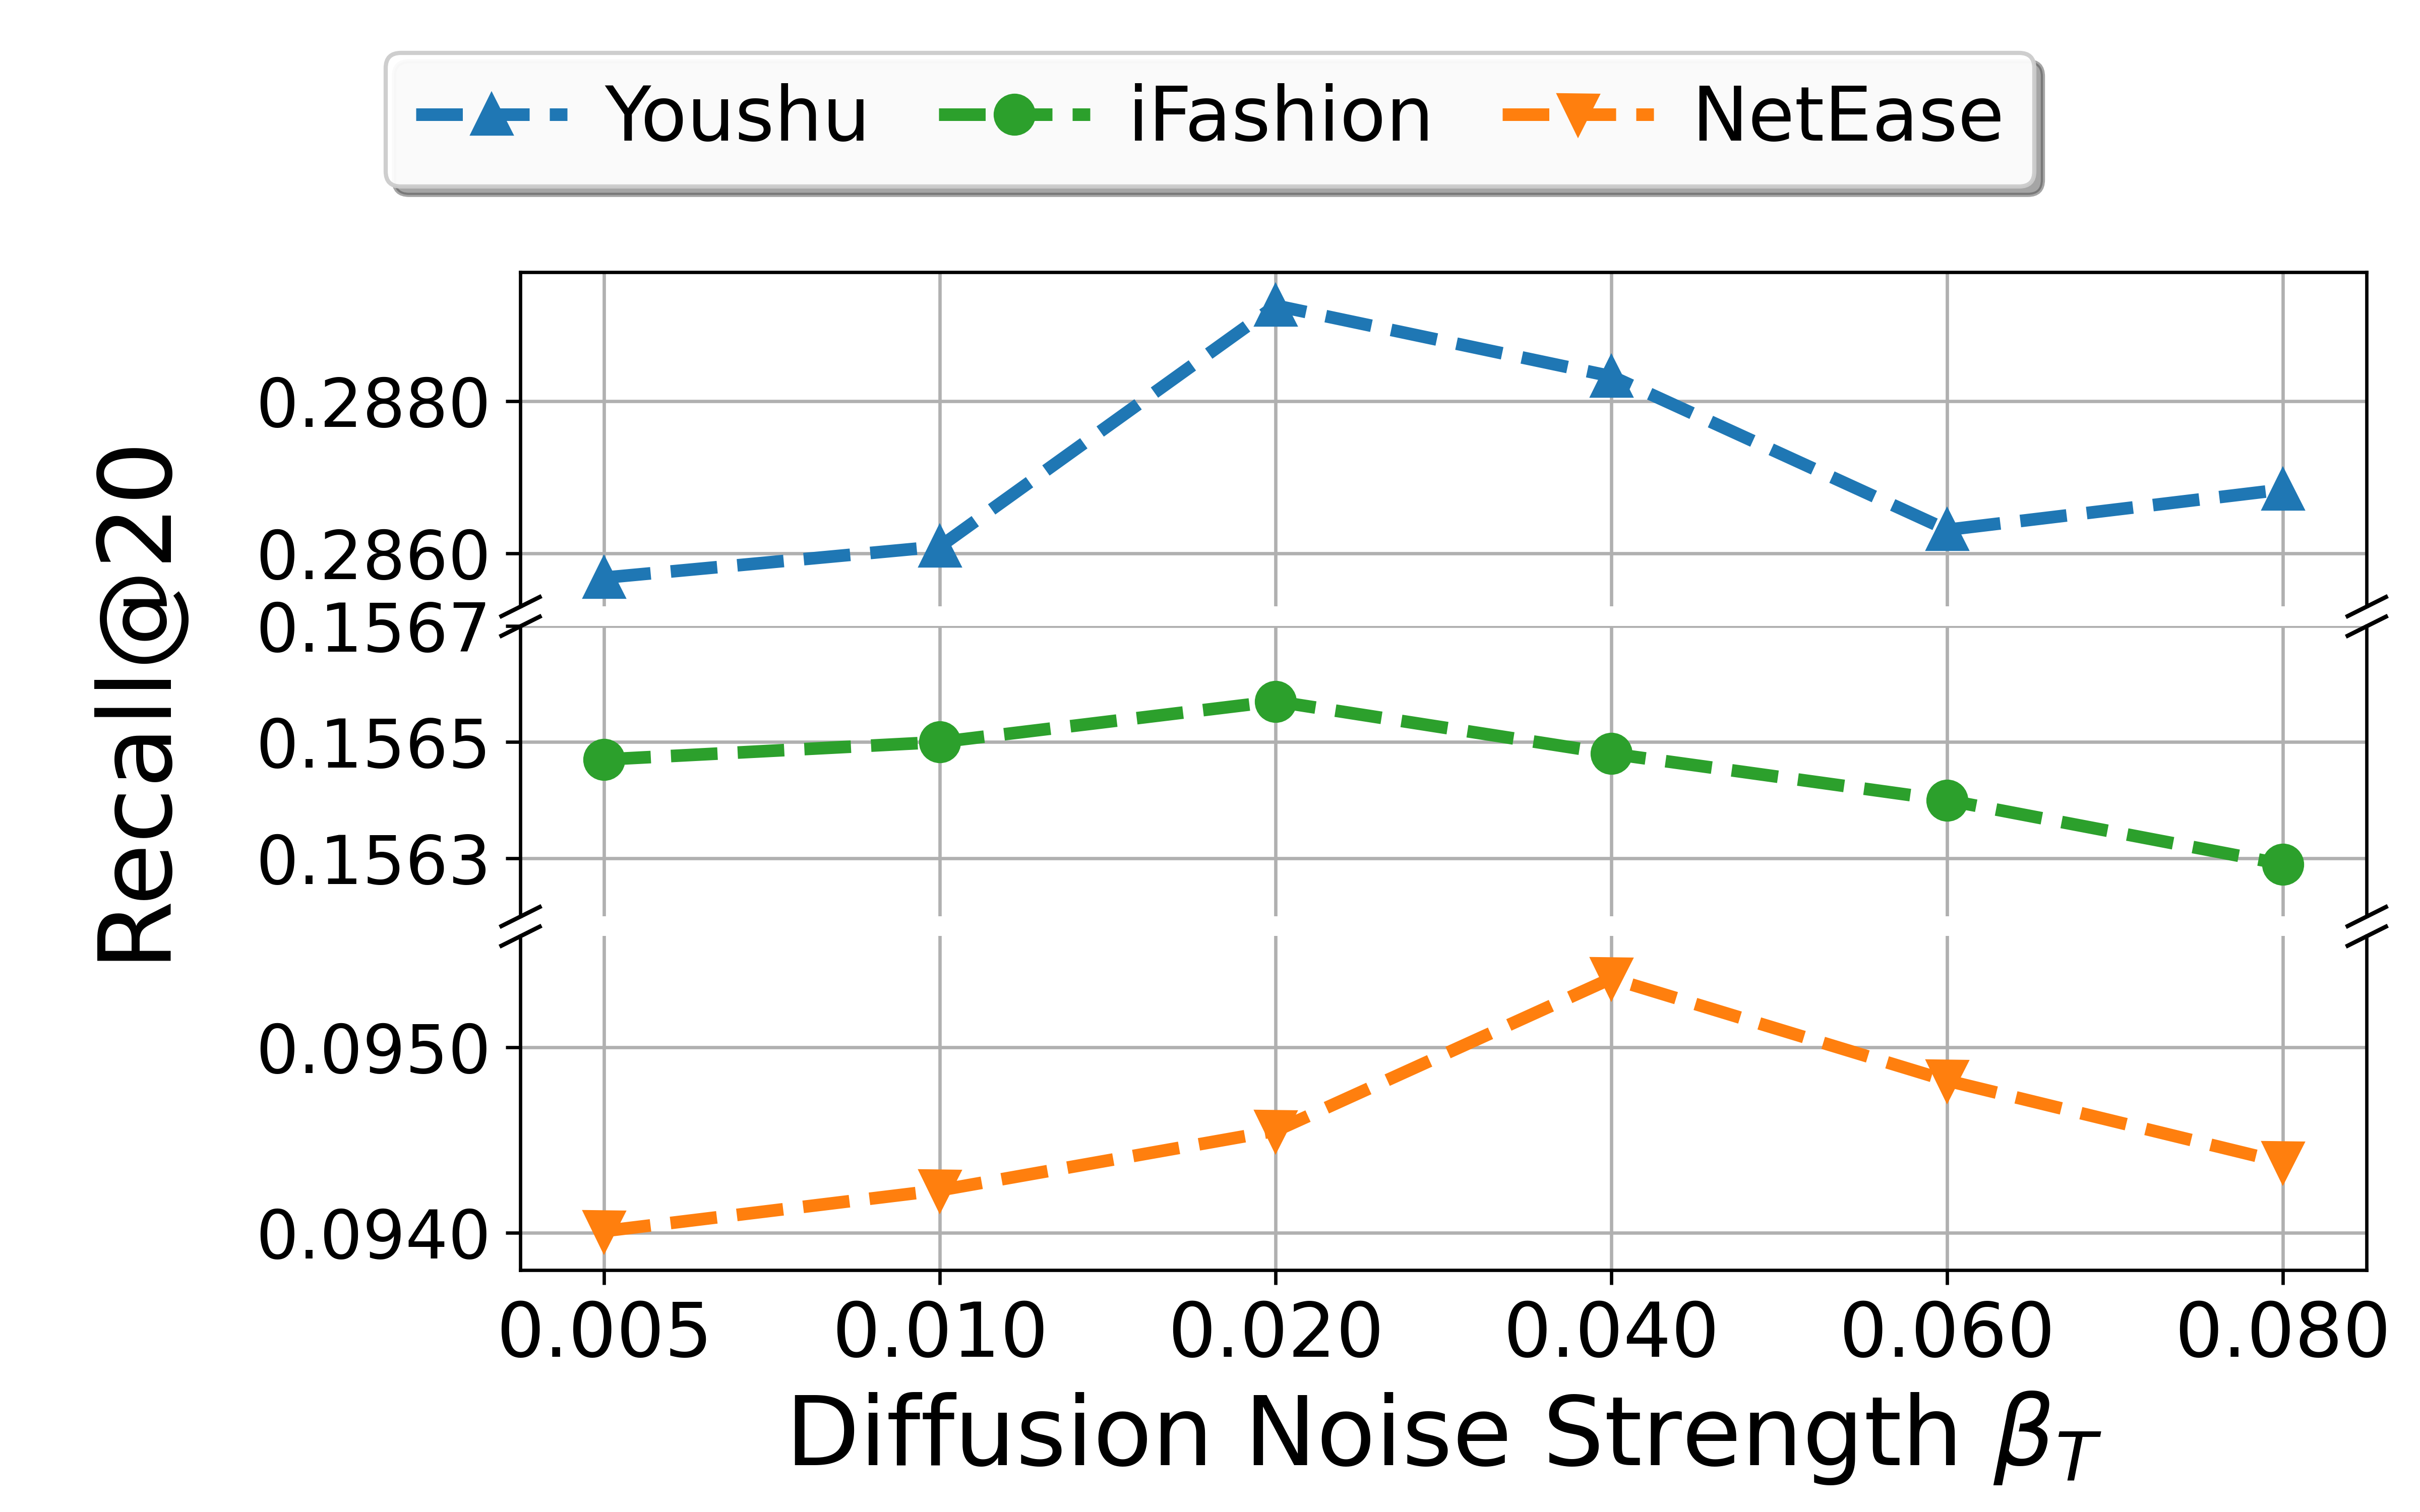
\includegraphics[width=0.285\textwidth]{Figures/hp_betaT.png} &
        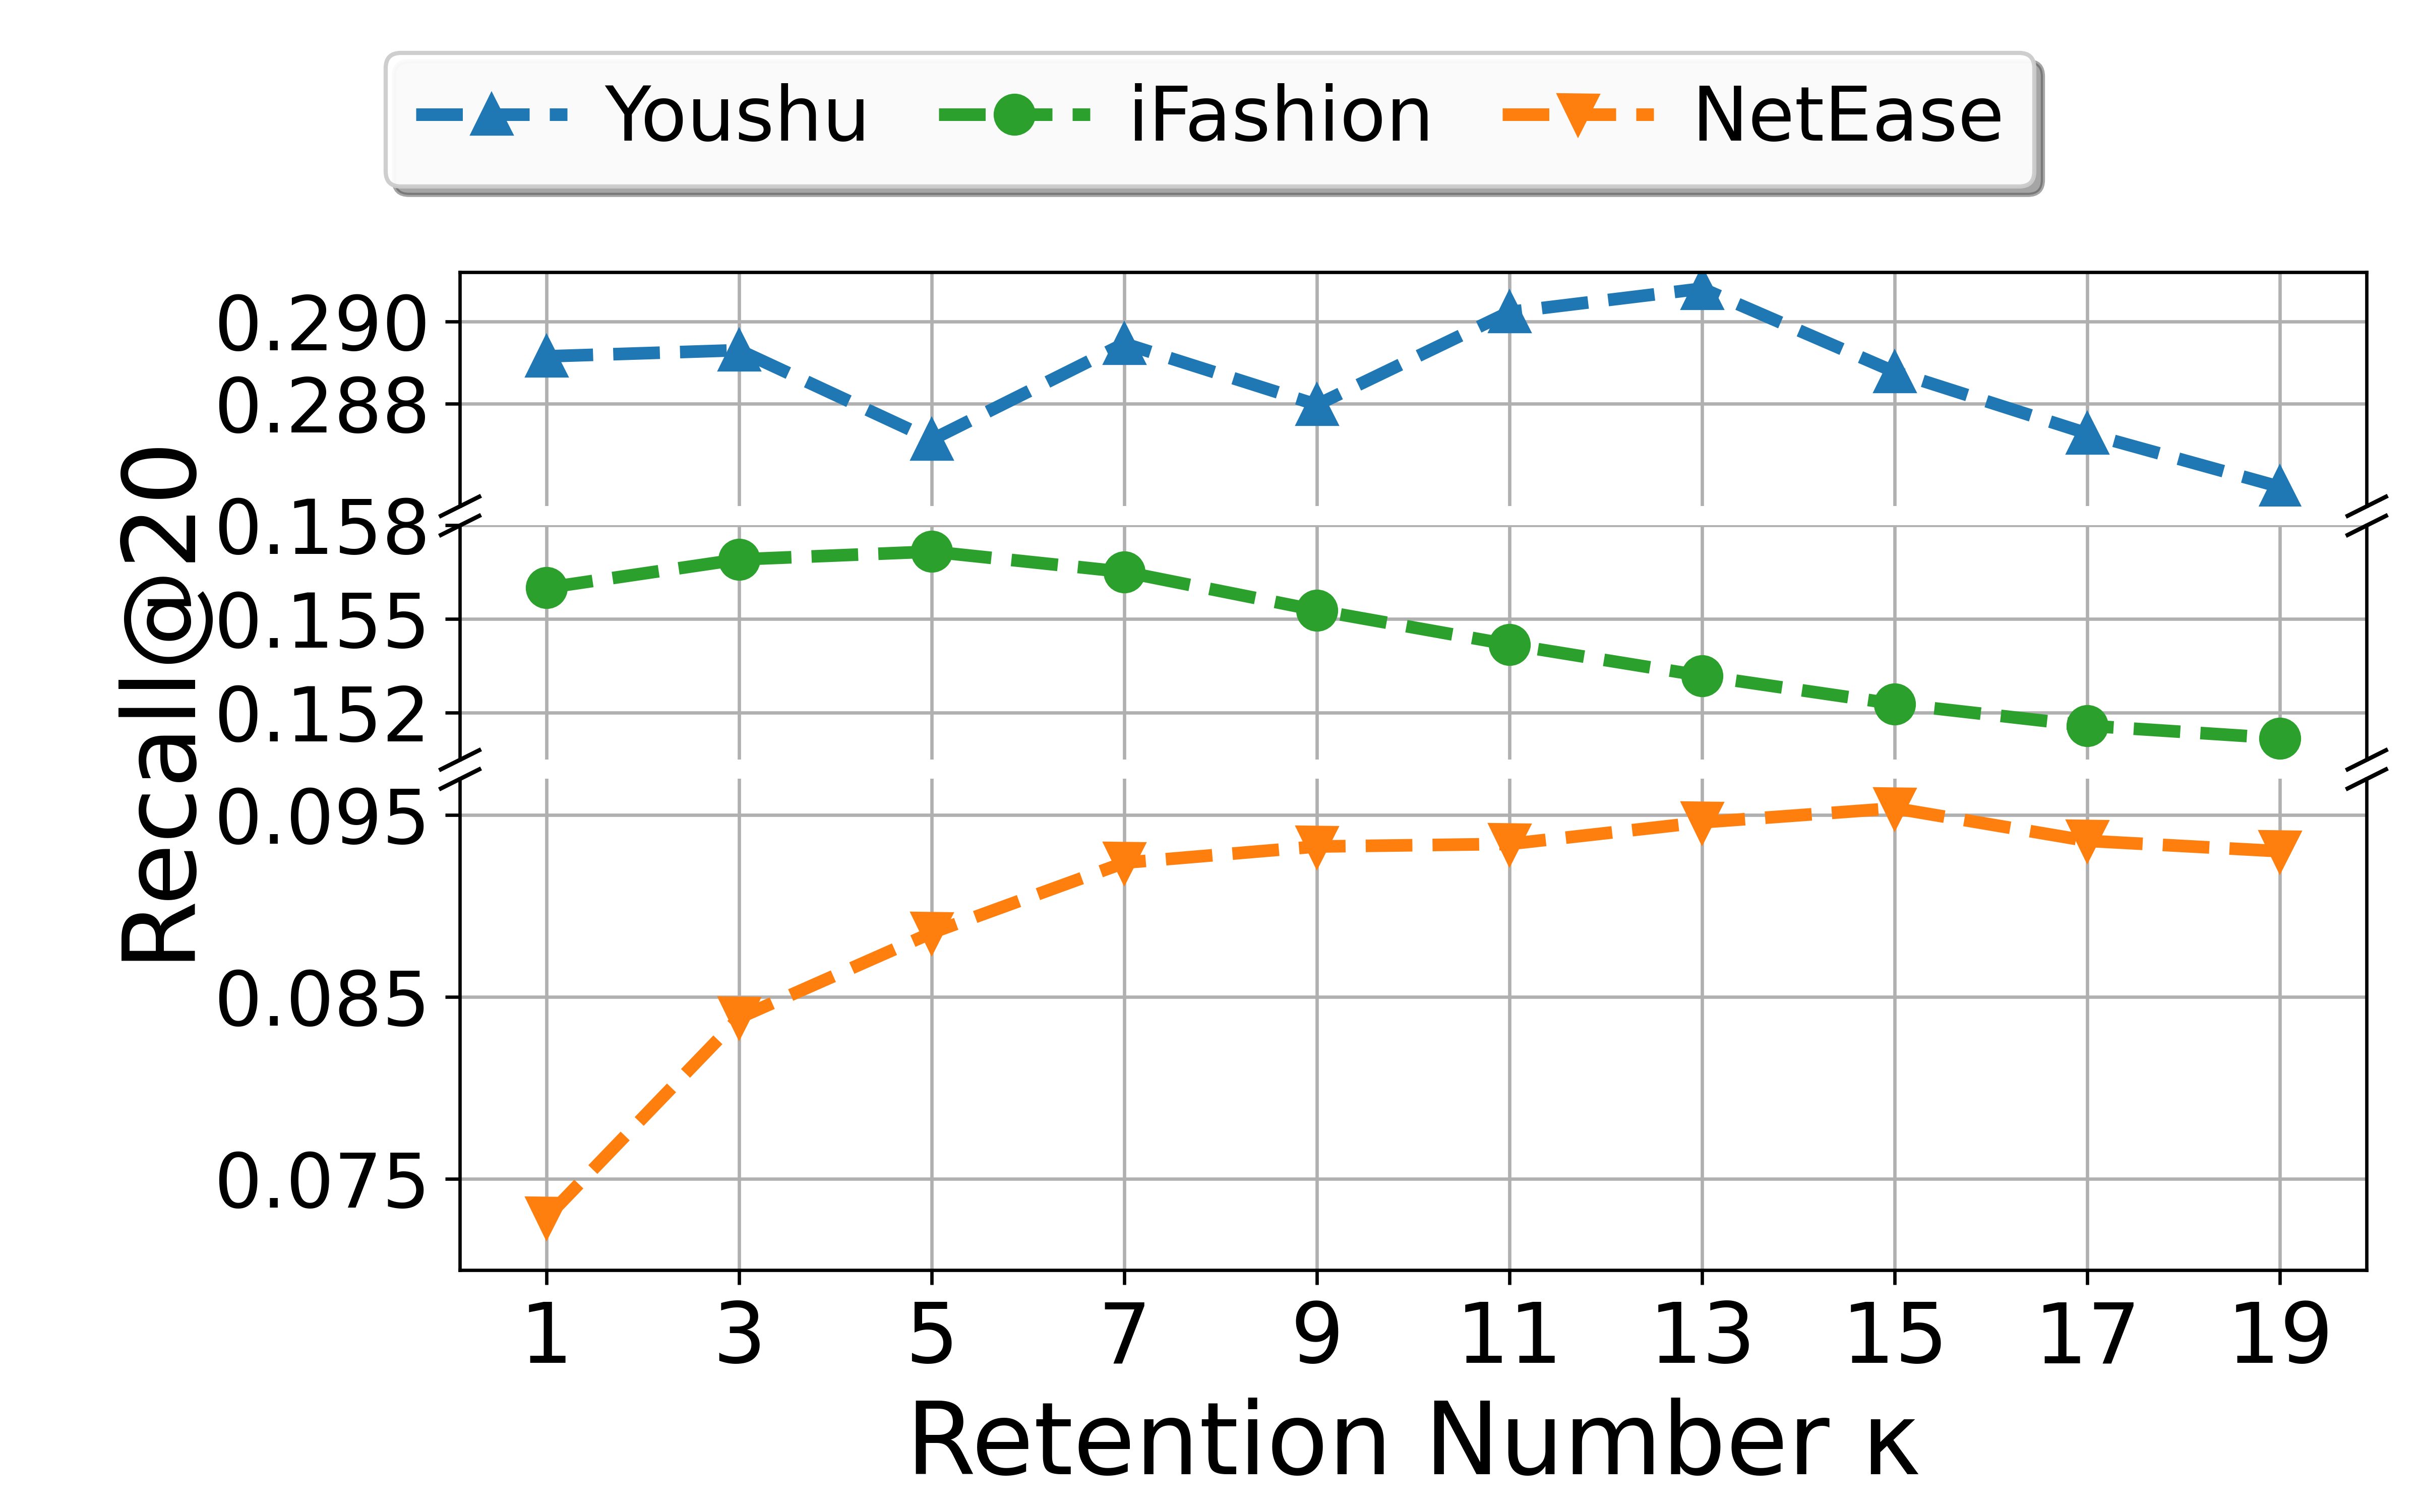
\includegraphics[width=0.285\textwidth]{Figures/hp_kappa.png} &
        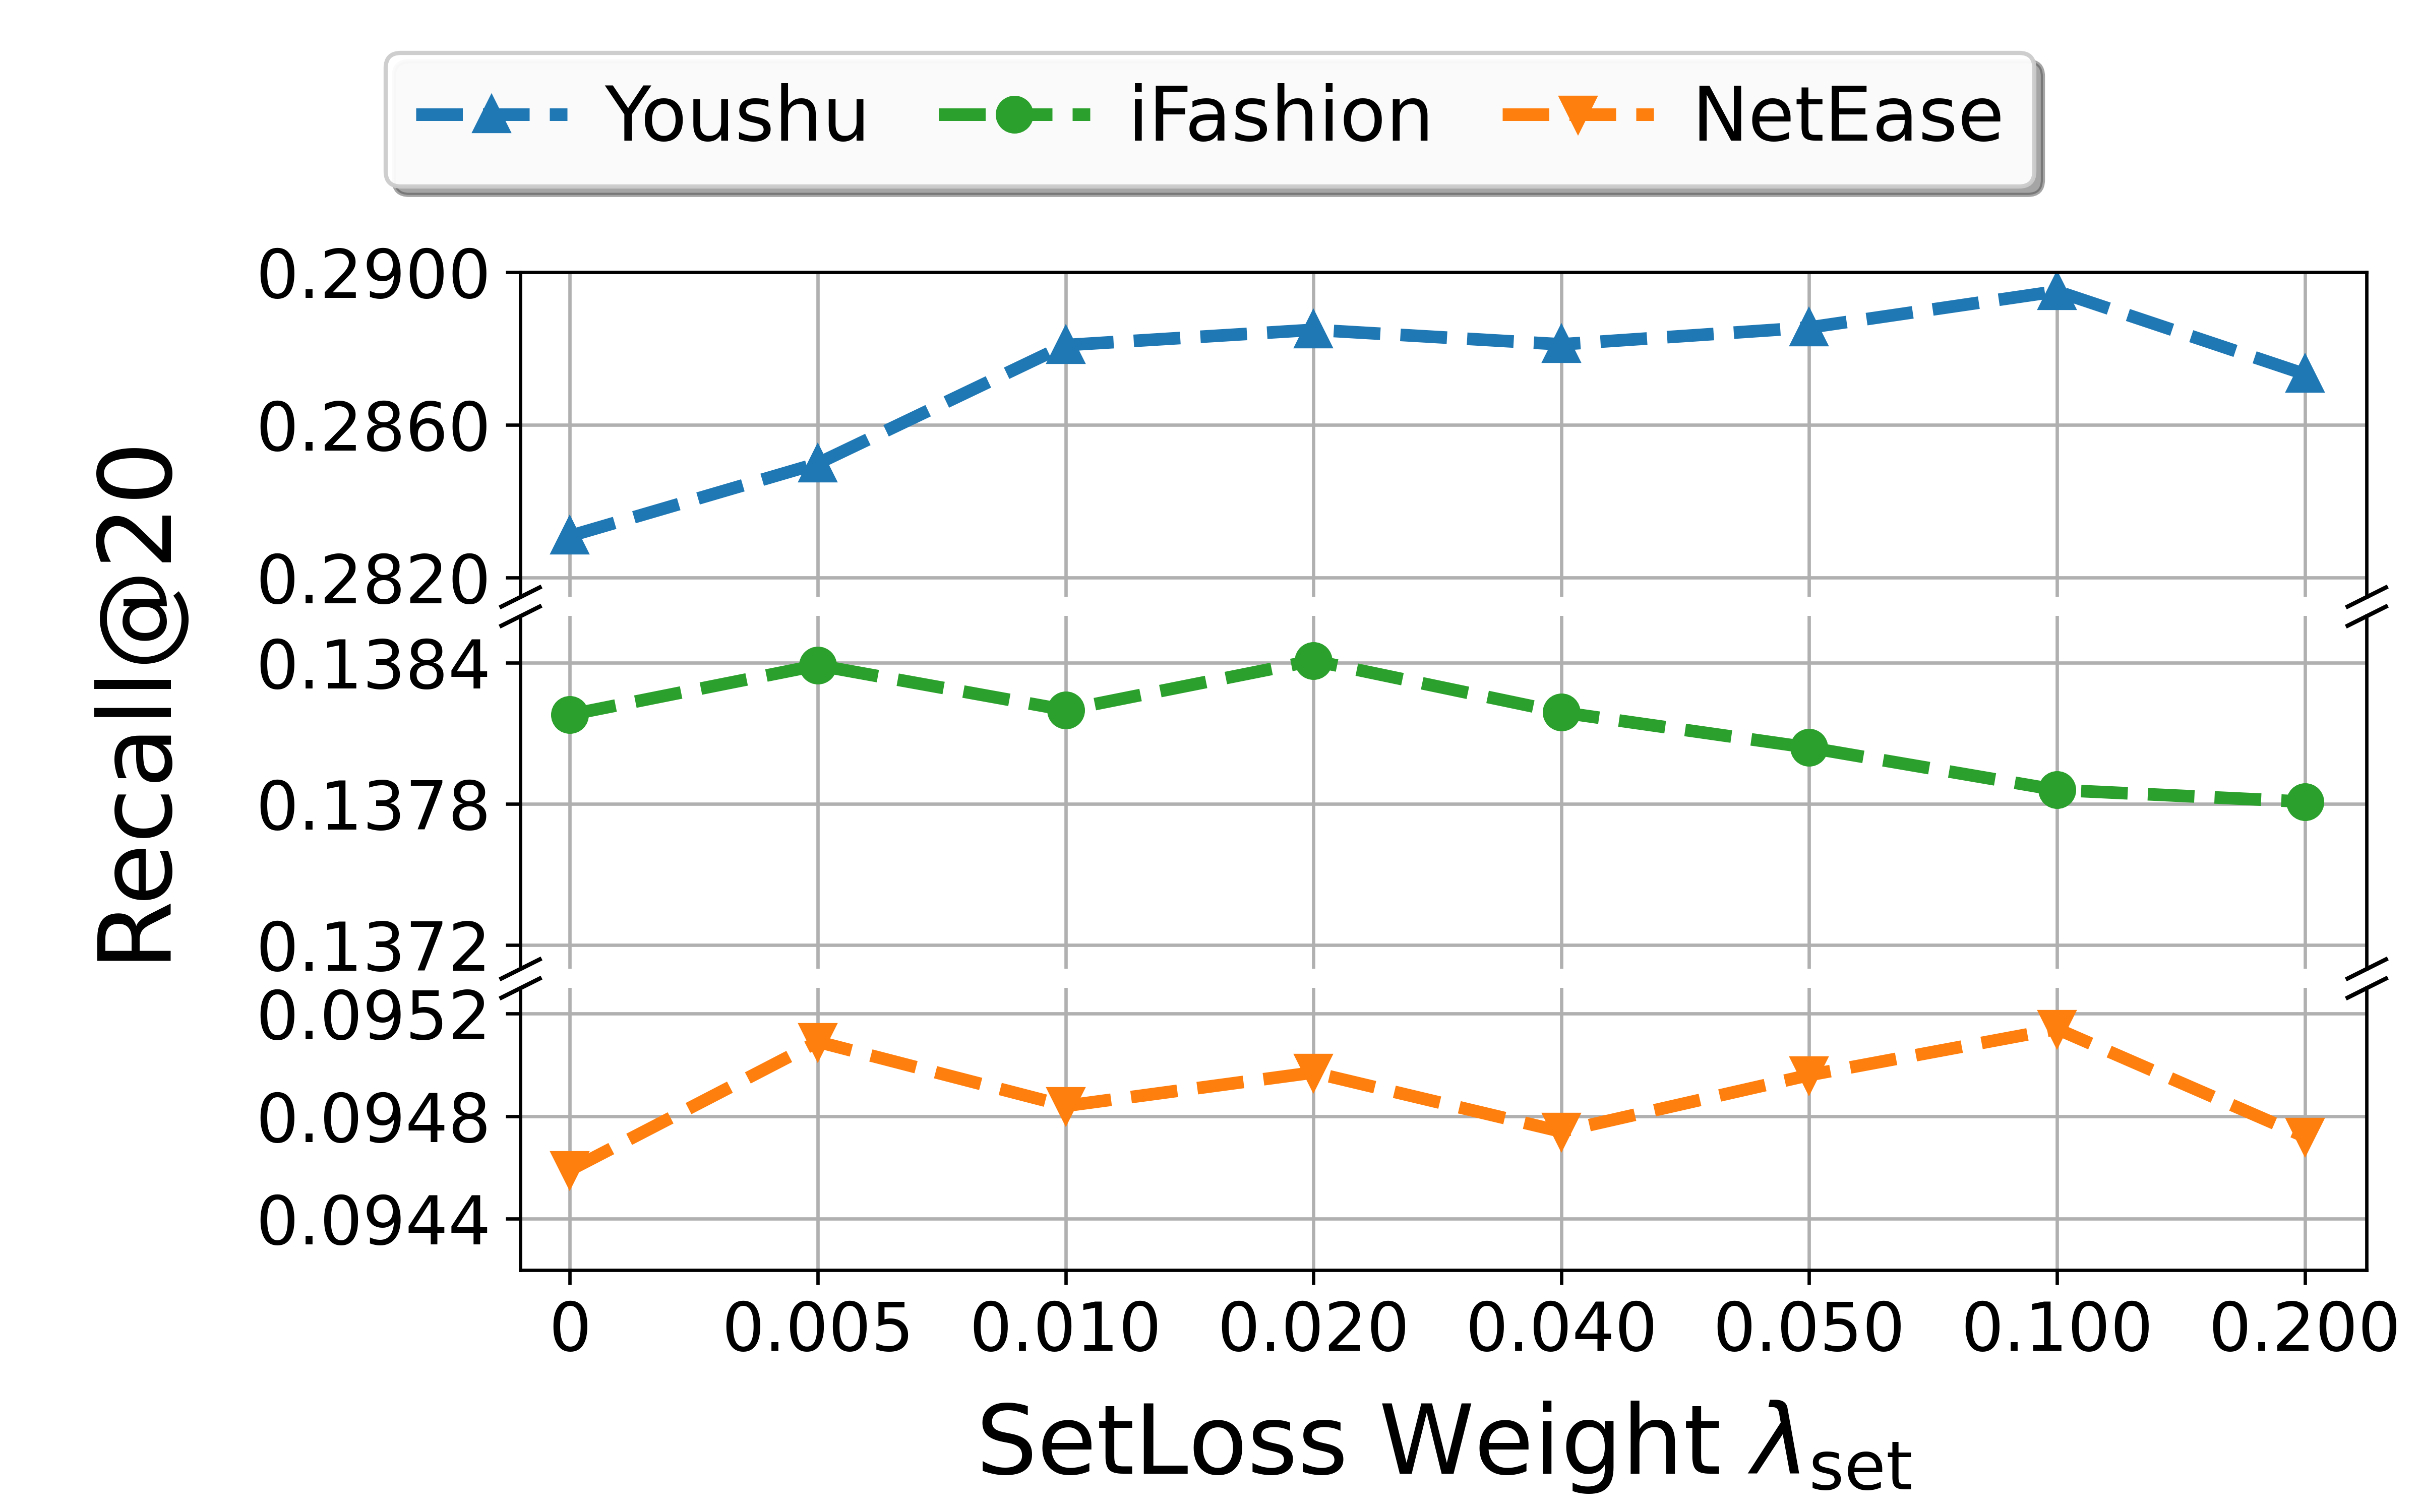
\includegraphics[width=0.285\textwidth]{Figures/set_loss.png} \\
        (a) & (b) & (c)
    \end{tabular}\par\smallskip
    \begin{tabular}{@{}c@{\hspace{0.025\textwidth}}c@{}}
        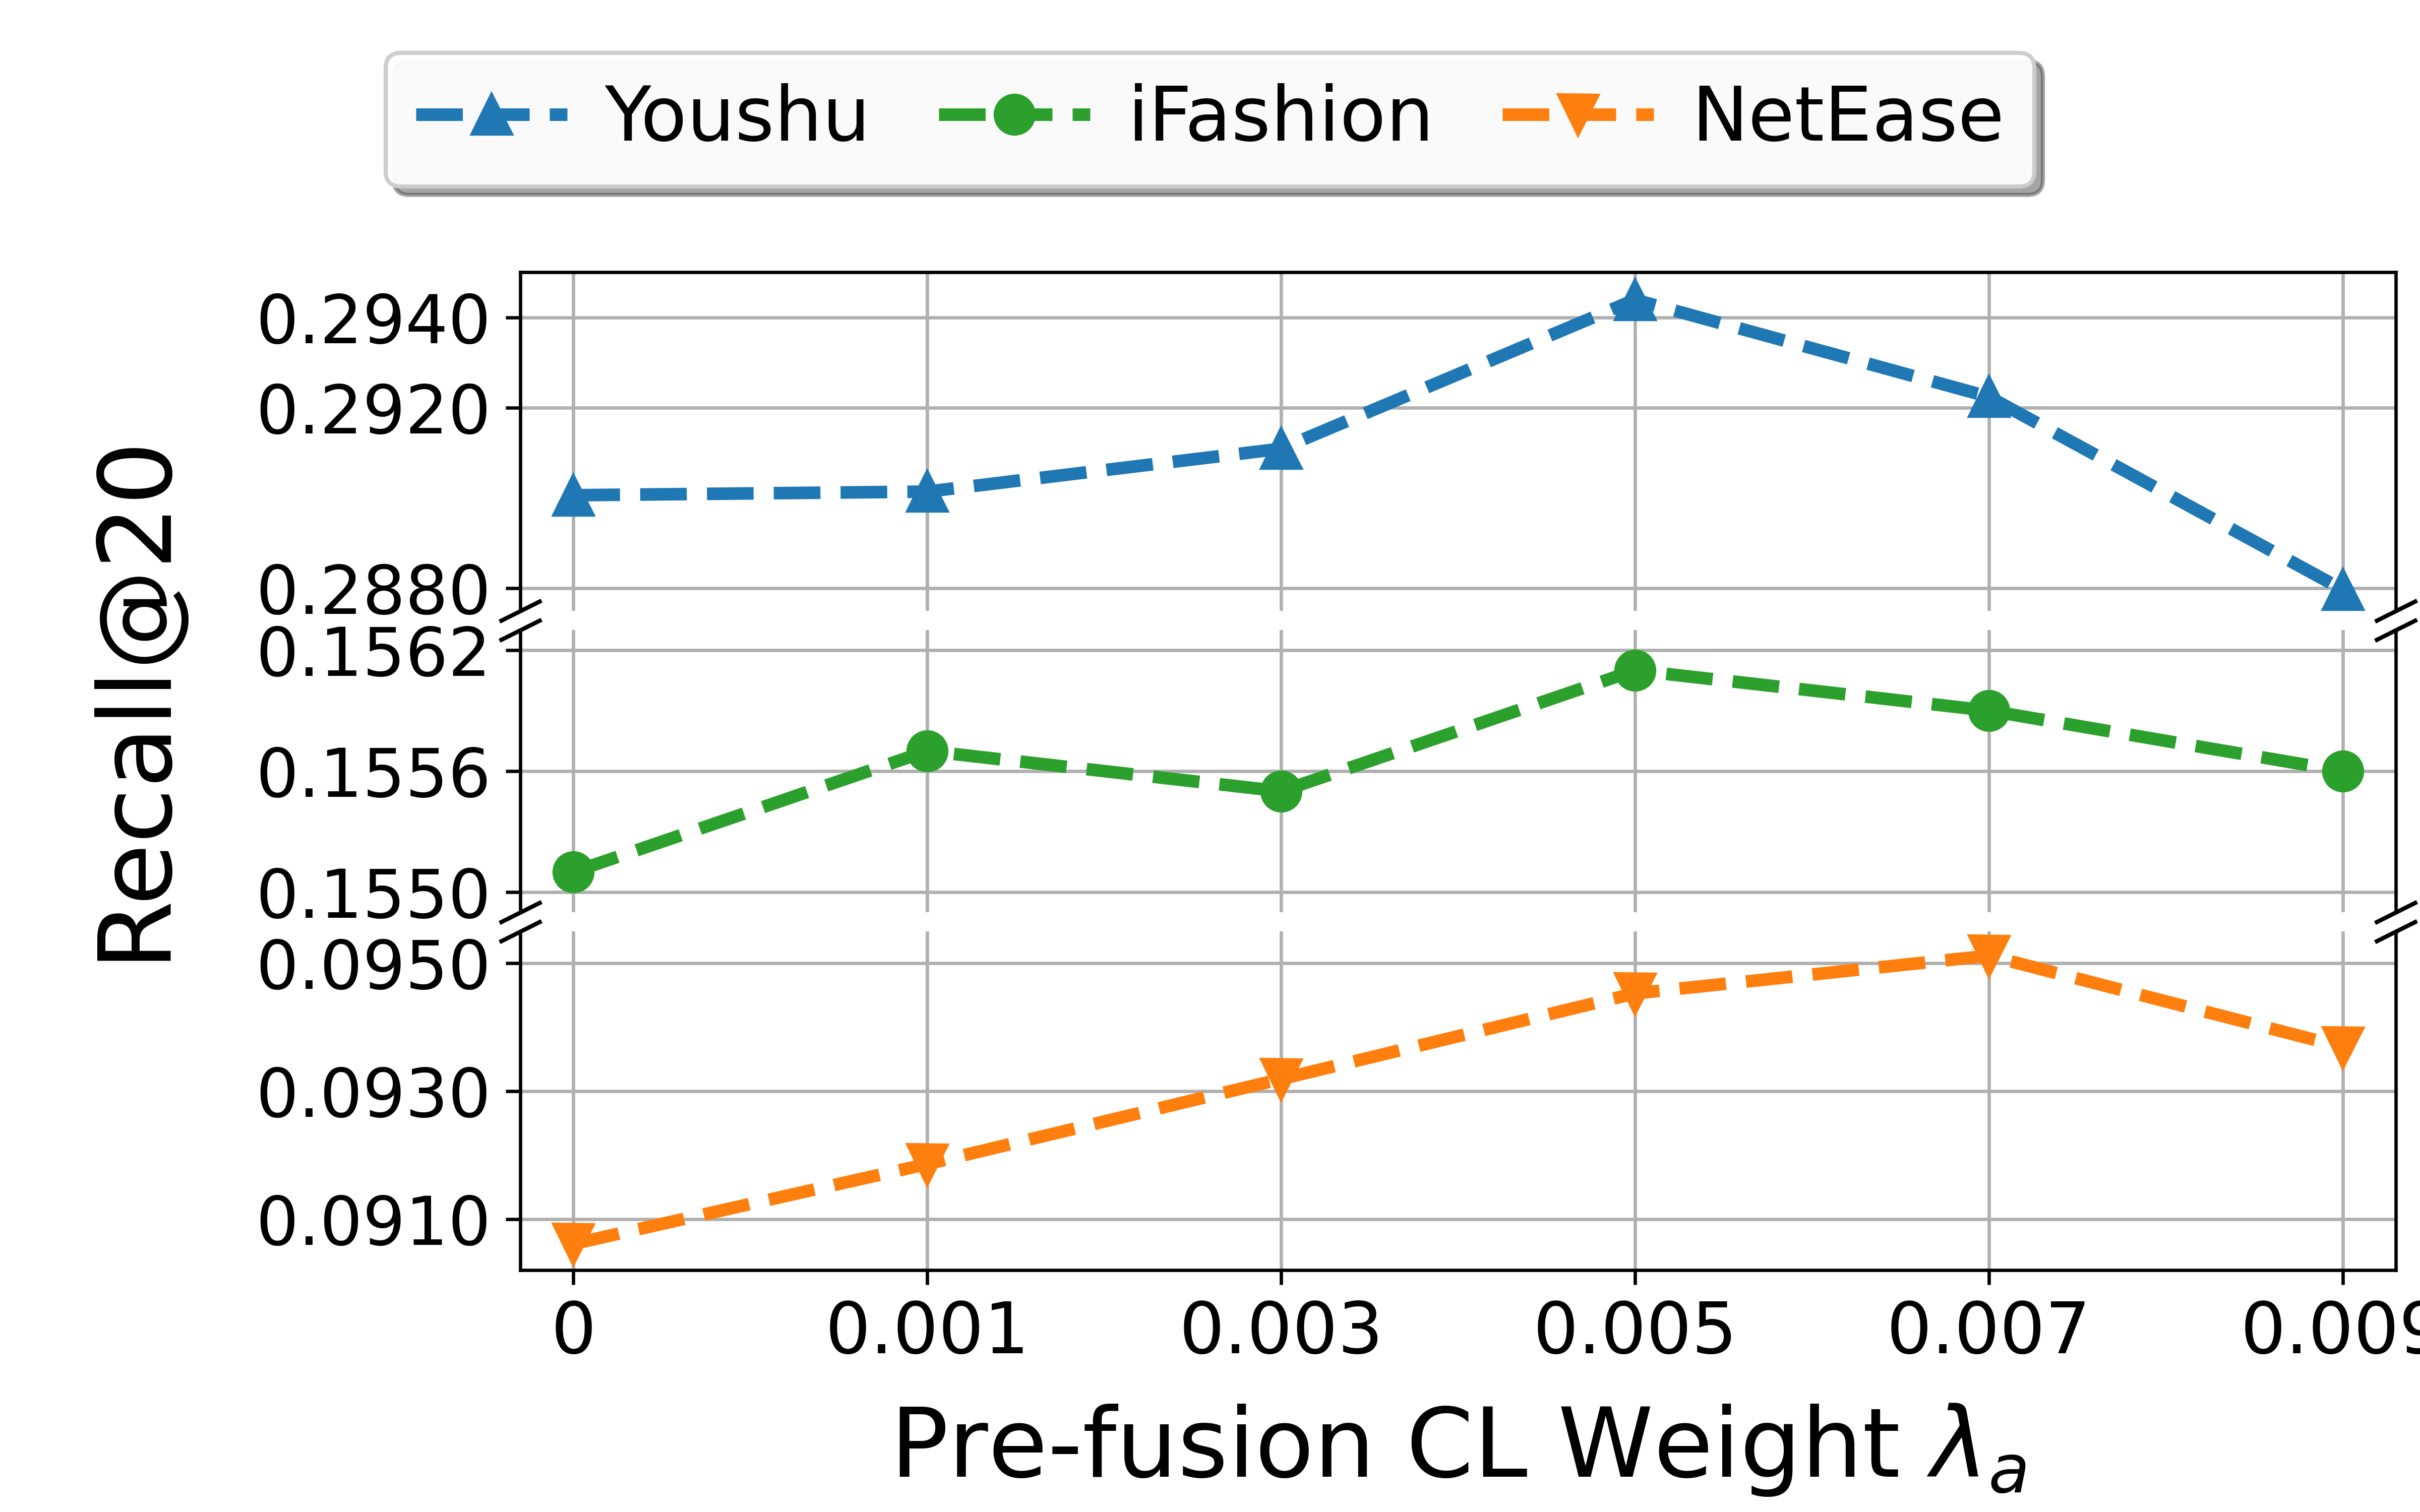
\includegraphics[width=0.285\textwidth]{Figures/hp_beta2.png} &
        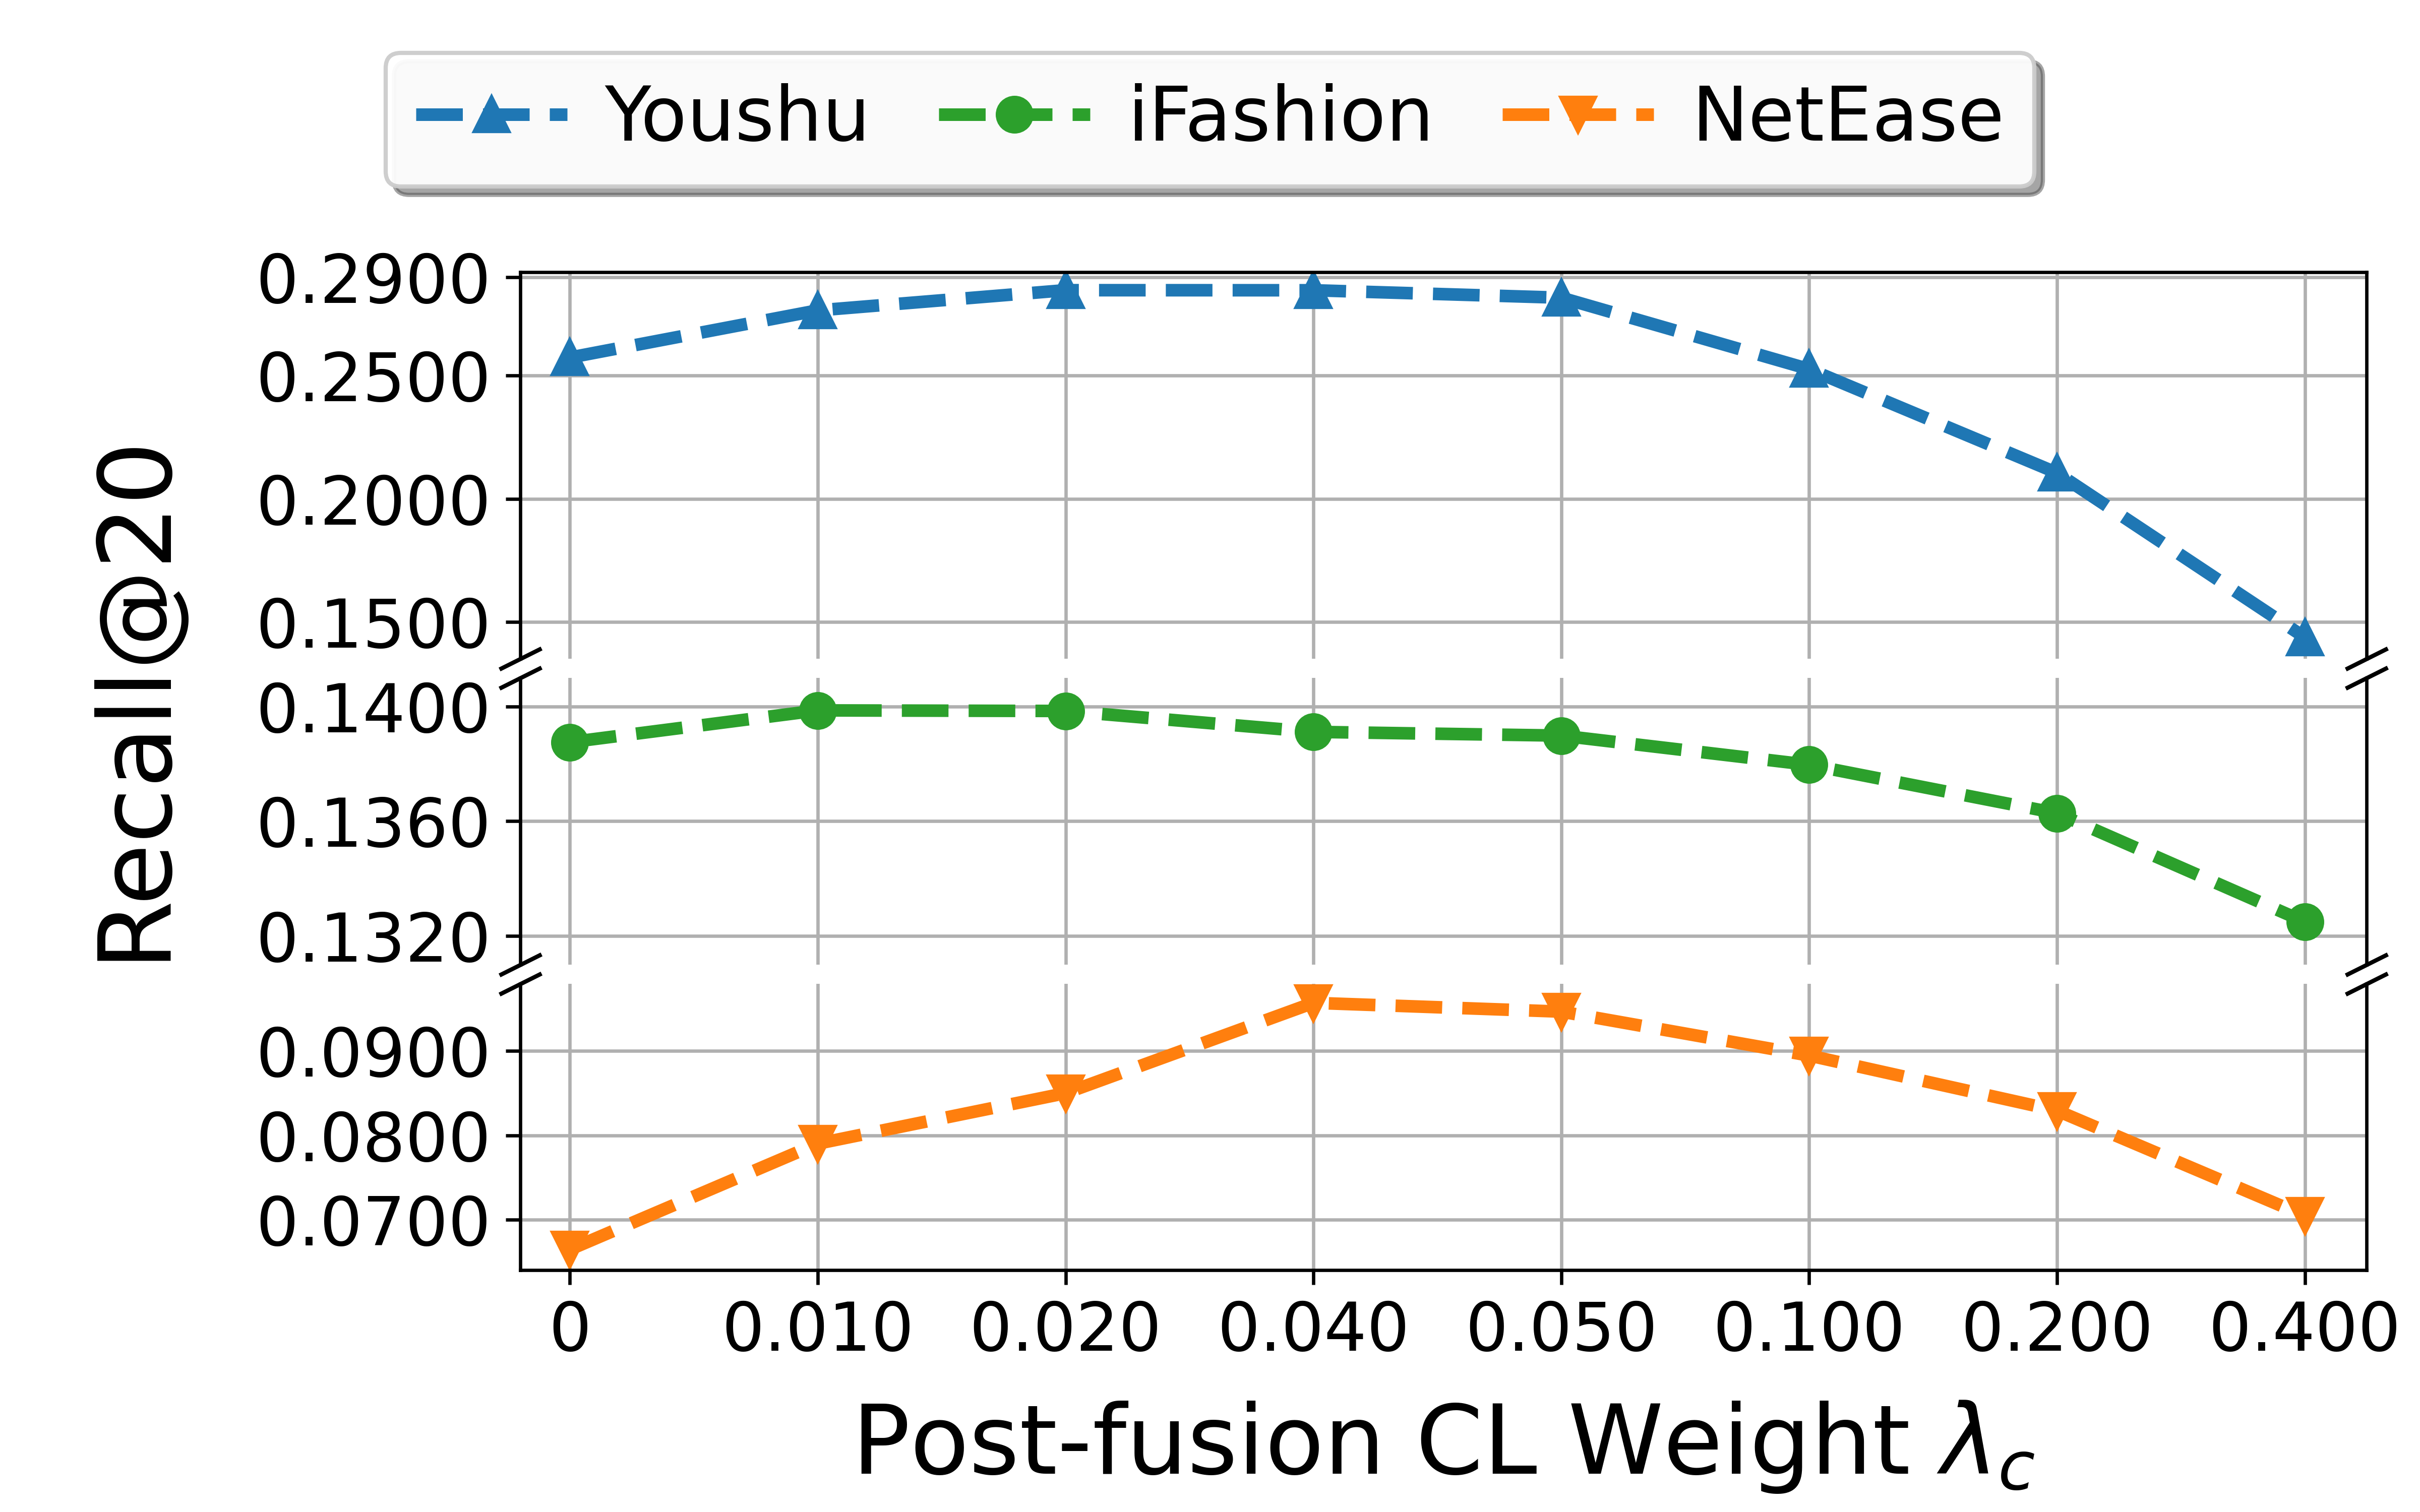
\includegraphics[width=0.285\textwidth]{Figures/post_fusion_cl.png} \\
        (d) & (e)
    \end{tabular}

    \caption{Hyperparameter sensitivity in Recall@20 on Youshu,
    iFashion, and NetEase. (a) Diffusion noise variance endpoint
    $\beta_T$. (b) U-B retention limit $\kappa$.
    (c) SetLoss weight $\lambda_{\mathrm{set}}$.
    (d) Pre-fusion contrastive weight $\lambda_a$.
    (e) Post-fusion contrastive weight $\lambda_c$.
    Broken $y$-axes use different scales for the datasets;
    candidate values are displayed at equally spaced horizontal
    positions.}
    \label{fig:hyperparameter}
\end{figure*}

\paragraph{Interaction Selection Strategies}
To examine how the selection strategy affects recommendation,
we compare ReCoBR with four variants on iFashion.
\textbf{Original UB} uses the observed U-B graph without filtering.
The other variants filter connections using random selection
(\textbf{Random-K}), bundle popularity (\textbf{Popularity-K}),
or pretrained user-bundle similarity (\textbf{Pretrain-Sim}).
All filtering strategies select from users' training histories
under the same per-user retention limit $\kappa$.
Fig.~\ref{fig:interaction-selection} shows that ReCoBR achieves
the highest Recall@20 and NDCG@20 at all tested retention limits.
Random-K can improve over Original UB, but its gap from ReCoBR
indicates that the selection criterion matters beyond reducing
the number of connections. Popularity-K's low NDCG@20 reflects
the limitations of global popularity for personalized ranking.
Pretrain-Sim also performs worse than Random-K, showing the
limitations of directly using pretrained user-bundle similarity
for interaction selection. In contrast, PDGR constructs and
denoises historical preference representations before scoring
connections, providing a more effective basis for graph reconstruction.

\paragraph{Performance on Sparse Users}
To evaluate CCL for sparse users, we sort NetEase users by
increasing training U-B interaction counts and divide them
into four equally sized groups (G1--G4). We compare ReCoBR
with \textbf{w/o CCL}, retaining PDGR in both.
Fig.~\ref{fig:sparse-users} shows improvements across all
four groups, with the largest relative gains in the sparsest
group G1: 12.64\% in Recall@20 and 9.32\% in NDCG@20.
The larger gains in G1 indicate that additional cross-view
supervision is particularly useful when users have few historical
bundle interactions.

\paragraph{Robustness to Noisy U-B Interactions}
To evaluate robustness to noisy interactions, we add random
U-B connections at noise ratios from 0\% to 25\%.
For each dataset and noise ratio, ReCoBR, CrossCBR, and
MultiCBR use the same perturbed U-B input graph.
We keep the original training interactions as ranking supervision
and leave the U-I and B-I relations and evaluation data unchanged.
We rerun ReCoBR's full training pipeline, including U-B pretraining.

As shown in Fig.~\ref{fig:noise-robustness}, ReCoBR maintains
the highest Recall@20 and NDCG@20 across all datasets and
tested noise ratios. By filtering connections using denoised
preferences, PDGR helps reduce the influence of noisy interactions
during neighborhood aggregation.

\subsection{Hyperparameter Sensitivity}

Fig.~\ref{fig:hyperparameter} reports ReCoBR's sensitivity
to five key hyperparameters. We vary one parameter at a time
while keeping the others fixed. For the noise variance endpoint
$\beta_T$, intermediate values yield better performance than
the extremes, suggesting that preference recovery benefits
from moderate perturbation. A smaller retention limit $\kappa$
works better on iFashion, whereas NetEase benefits from
retaining more connections. This difference illustrates the
tradeoff between retaining useful history and including less
relevant connections in graph propagation. Nonzero
SetLoss weights $\lambda_{\mathrm{set}}$ improve performance
on Youshu, while iFashion and NetEase show only small,
nonmonotonic changes. Increasing this weight does not
consistently yield further gains.

For the CCL weight $\lambda_a$, moderate nonzero values improve
performance, while larger values can reduce it. Similarly, post-fusion
contrastive learning benefits from a moderate $\lambda_c$.
Larger weights cause pronounced performance drops on Youshu
and NetEase, highlighting the need to balance the contrastive
and ranking objectives.

\section{Conclusion}

In this paper, we proposed ReCoBR to address noisy and sparse
U-B interactions in bundle recommendation. PDGR denoised historical
preference representations from pretrained embeddings with a
user-conditioned diffusion model, using SetLoss to help retain
useful preference information. The denoised preferences then
guided U-B interaction filtering and graph reconstruction.
Building on the reconstructed graph, CCL introduced cross-view
constraints before representation fusion to improve bundle
preference learning for sparse users. In experiments on three
public datasets, ReCoBR outperformed the baseline methods.
Further analyses showed improvements for sparse users and a
consistent recommendation advantage under noisy U-B interactions.

\bibliographystyle{IEEEtran}
\bibliography{references}

\end{document}
